\pdfminorversion=5 
\pdfcompresslevel=9
\pdfobjcompresslevel=2

\documentclass[12pt]{aghdpl}
%\documentclass[language=en,11pt]{aghdpl}  % praca w języku angielskim

%\usepackage[MeX]{polski}
%\usepackage[hidelinks]{hyperref}
%\usepackage{color}
%\usepackage{mathtools}
%\usepackage[OT4]{fontenc}
%\usepackage{listings}
%\usepackage[margin=1in]{geometry}
%\usepackage{float}
%\floatstyle{plaintop}
%\restylefloat{table}
%\usepackage{breqn}
\usepackage{wrapfig}
\usepackage[hidelinks]{hyperref}
\usepackage{enumitem}
\setlist[itemize]{noitemsep}

%--------------------------------------------------------------------------
\usepackage{listings}
\usepackage{xcolor}

\usepackage{MnSymbol}

\usepackage{float}

\usepackage{soul}
\definecolor{Light}{gray}{.90}
\sethlcolor{Light}
\let\OldTexttt\texttt
\renewcommand{\texttt}[1]{\OldTexttt{\hl{#1}}}

\definecolor{codegreen}{rgb}{0,0.6,0}
\definecolor{codegray}{rgb}{0.5,0.5,0.5}
\definecolor{codepurple}{rgb}{0.58,0,0.82}
\definecolor{backcolour_python}{rgb}{0.97,1,0.95}
\definecolor{backcolour_bash}{rgb}{0.94,0.94,0.94}
\definecolor{backcolour_xml}{rgb}{1,0.93,0.93}
\definecolor{backcolour}{rgb}{0.97,1,0.9}

\lstset{
  literate={ą}{{\k a}}1
  		     {Ą}{{\k A}}1
           {ż}{{\. z}}1
           {Ż}{{\. Z}}1
           {ź}{{\' z}}1
           {Ź}{{\' Z}}1
           {ć}{{\' c}}1
           {Ć}{{\' C}}1
           {ę}{{\k e}}1
           {Ę}{{\k E}}1
           {ó}{{\' o}}1
           {Ó}{{\' O}}1
           {ń}{{\' n}}1
           {Ń}{{\' N}}1
           {ś}{{\' s}}1
           {Ś}{{\' S}}1
           {ł}{{\l}}1
           {Ł}{{\L}}1
}
% https://gist.github.com/KKozlowski/bd2c2267ea68fd5f92c30ac5ebeb2f16

\lstset{prebreak=\raisebox{0ex}[0ex][0ex]
        {\ensuremath{\rhookswarrow}}}
\lstset{postbreak=\raisebox{0ex}[0ex][0ex]
        {\ensuremath{\rcurvearrowse\space}}}

\lstset{
    backgroundcolor=\color{backcolour},   
    commentstyle=\color{codegreen},
    keywordstyle=\color{blue},
    numberstyle=\tiny\color{codegray},
    stringstyle=\color{orange},
    basicstyle=\ttfamily\footnotesize,
    breakatwhitespace=false,
    breaklines=true,
    captionpos=b,
    keepspaces=false,
    numbers=none,
    showspaces=false,                
    showstringspaces=false,
    showtabs=false,
    tabsize=2,
    columns=fullflexible,
}

\lstdefinestyle{C}{
  language=C,
  numbers=left,
  stepnumber=1,
  frame=single,
  backgroundcolor=\color{backcolour},
  xleftmargin=\parindent,
  morekeywords={int32_t, uint32_t},
}

\lstdefinestyle{Matlab}{
  language=Matlab,
  numbers=left,
  stepnumber=1,
  frame=single,
  backgroundcolor=\color{backcolour},
  xleftmargin=\parindent,
  morekeywords={self, yield},
}

%---------------------------------------------------------------------------

\author{inż. Jakub Mazur}
\shortauthor{J. Mazur}


\titlePL{System pozycjonowania wibrometru laserowego}
\titleEN{Laser vibrometer positioning system}


\shorttitlePL{System pozycjonowania wibrometru laserowego} % skrócona wersja tytułu jeśli jest bardzo długi
\shorttitleEN{Laser vibrometer positioning system}


% Dopuszczalne wartości[1,2]:
% * "Projekt dyplomowy" - na koniec studiów I stopnia
% * "Praca dyplomowa" - na koniec studiów II stopnia
% [1] Zasady dyplomowania w roku akademickim 2020/2021 (Decyzja Dziekana WEAIiIB nr 16/2020 z dnia 9 grudnia 2020 roku)
% [2] Załącznik nr 1a) do Decyzji nr 16/2020 Dziekana Wydziału EAIiIB z dnia 09 grudnia 2020 r.
\thesistype{Praca dyplomowa}
%\thesistype{Master of Engineering Thesis}

%\supervisor{Artur Flach, BEng, PhD}
\supervisor{dr inż. Artur Flach}

%\degreeprogramme{Acoustical Engineering}
\degreeprogramme{Inżynieria Akustyczna}

\date{2024}

%\department{Katedra Informatyki Stosowanej}
%\department{Department of Applied Computer Science}

%\faculty{Faculty of Mechanical Engineering and Robotics}
\faculty{Wydział Inżynierii Mechanicznej i Robotyki}

\acknowledgements{Serdecznie dziękuję mojemu Promotorowi Dr Inż. Arturowi Flachowi, za wsparcie, zaangażowanie i merytoryczną pomoc przy tworzeniu pracy. Chciałbym także podziękować całemu zespołowi, z którym pracowałem nad projektem WWE w kole naukowym Integra, za pomoc w wyborze technologii użytych w pracy.}


\begin{document}
    \newenvironment{abstractpage}
    {\cleardoublepage\vspace*{\fill}\thispagestyle{empty}}
    {\vfill\cleardoublepage}
    \renewenvironment{abstract}[1]
    {\bigskip\selectlanguage{#1}%
    \begin{center}\bfseries\abstractname\end{center}}
    {\par\bigskip}
	\titlepages

	\begin{abstractpage}
    \begin{abstract}{polish}
        Celem pracy było zaprojektowanie systemu, pozwalającego na przeprowadzanie pomiarów skanujących za pomocą wibrometru punktowego. W ramach pracy miała powstać konstrukcja, wraz z oprogramowaniem pozwalającym na jej sterowanie.

        Rezultatem pracy był wydrukowany w technologii 3D oraz wykonany na CNC ruchomy stół, pozwalający na ruch dookoła dwóch osi, yaw (z) oraz pitch (y). Dodatkowo, używając bibliotek Zephyr RTOS, zaimplementowane zostało oprogramowanie w języku C, pozwalające na osiąganie przez system kolejnych pozycji i dokonywania skanów powierzchni. Aby umożliwiać prostszą interakcję z urządzeniem, powstało API w języku Matlab, oraz aplikacja desktopowa z GUI w języku C\#.

        Testy wykazały, że skanowanie obiektów przy pomocy wibrometru punktowego, oraz skonstruowanego urządzenia, daje oczekiwane rezultaty.
        
        \bigskip
        \textbf{Słowa kluczowe:} Systemy Embedded, Wibrometria Punktowa, Wibrometria Skanująca, Język C, Zephyr RTOS
    \end{abstract}
    % \newpage
    \begin{abstract}{english}
        The aim of the work was to design a system that would allow scanning measurements to be taken using a point vibrometer. The work was to design a structure, along with software to control it.

        The result of the work was a 3D printed and CNC fabricated moving table, allowing movement around two axes, yaw (z) and pitch (y). In addition, C-language software was implemented using Zephyr RTOS libraries, allowing the system to reach successive positions and scan surfaces. To enable simpler interaction with the device, an API was developed in Matlab language, and a desktop application with a GUI in C\# language.

        Tests have shown that scanning objects with the point vibrometer, using the constructed device, produces the expected results.
        
        \bigskip    
        \textbf{Keywords:} Embedded Systems, Laser Point Vibrometry, Laser Scanning Vibrometry, C-Language, Zephyr RTOS
    \end{abstract}
\end{abstractpage}	
	
	\RedefinePlainStyle
	
	\setcounter{tocdepth}{2}
	\tableofcontents
	\clearpage
	
	\chapter{Wstęp}
\label{cha:Intro}
Wibrometria laserowa to technika pomiarowa pozwalająca na bezkontaktowe pomiary drgań powierzchni. Opiera się ona na odbiciu wiązki lasera, z którego można odczytać drgania powierzchni. Ponieważ pojedyncza wiązka lasera mierzy drgania pojedynczego punktu, problemem przy wykonywaniu takich pomiarów jest skanowanie drgań większych powierzchni. Dlatego też celem tej pracy jest konstrukcja systemu, który pozwoli na użycie wibrometru punktowego do przeskanowania powierzchni.

\section{Wibrometria laserowa \cite{Polytec_LDV}}
Wibrometr (\textbf{Laser Doppler Vibrometer}; \textbf{LDV}) to instrument służący do bezkontaktowych pomiarów drgań powierzchni. Wiązka lasera jest kierowana na mierzony obiekt, po czym wiązka odbita jest falą, o nieznacznie innej częstotliwości i fazie niż wiązka oryginalna. Zmiana ta jest proporcjonalna do drgań (ruchu) powierzchni, od której wiązka się odbiła.

\begin{figure}[h!]
\centering
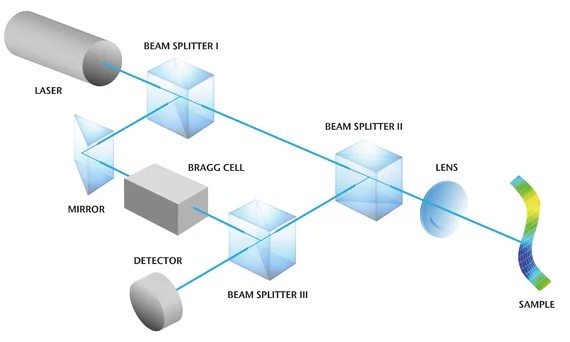
\includegraphics[width=0.8\textwidth]{img/ldv_inside.jpg}
\caption{Układ pomiarowy wewnątrz standardowego wibrometru laserowego. Źródło: \cite{Polytec_LDV}}
\label{img:ldv_inside}
\end{figure}

Wewnątrz wibrometru, rozdzielacz wiązki (Beam Splitter) rozdziela wiązkę laserową na wiązkę referencyjną oraz wiązkę pomiarową. Wiązka pomiarowa odbija się od mierzonego obiektu, po czym łączy się z wiązką referencyjną w operacji superpozycji i trafia na fotodetektor. (Przedstawione na rys. \ref{img:ldv_inside}.)

\subsection{Efekt Dopplera}
Podstawą działania wibrometru laserowego jest efekt Dopplera. Zgodnie z efektem Dopplera, zmiana częstotliwości wiązki pomiarowej względem wiązki odbitej jest proporcjonalna do szybkości ruchu obiektu oraz odwrotnie proporcjonalna do długości fali światła - zgodnie ze wzorem \ref{eq:doppler}. 

\begin{equation} \label{eq:doppler}
f_D = 2 \frac{v}{\lambda}
\end{equation}

Wzór \ref{eq:doppler} pozwala na wyznaczenie prędkości mierzonego obiektu na podstawie zmiany częstotliwości wiązki światła. Natomiast sama zmiana częstotliwości jest wyznaczana z superpozycji wiązek za pomocą interferometrii.

\subsection{Interferometria}
Wspomniano powyżej, że na fotodetektor trafia superpozycja wiązki referencyjnej oraz odbitej. Interferometria to technika stosująca interferencję fal w superpozycji do ekstrakcji informacji z tych fal, wykorzystywana właśnie w tym celu w wibrometrze. \cite{history_of_science_and_tech}

Przykładowo, jeżeli obie fale mają tą samą częstotliwość, interferencja dwóch fal pozwala na łatwe wyciągnięcie informacji o przesunięciu w fazie między tymi dwoma falami. Jeżeli fale zupełnie się wygasiły, oznacza to, że strzałka naszła się z węzłem i przesunięcie w fazie wynosi dokładnie pół długości fali.Jeżeli strzałki się wzmocniły, oznacza to, że nie ma przesunięcia w fazie. Natomiast w każdym innym wypadku można łatwo obliczyć przesunięcie na podstawie pozycji węzłów i strzałek nowej fali. \cite{Two_laser_interferometry}

W przypadku wibrometrów laserowych, mierzona jest interferencja intensywności światła wiązek, zgodnie ze wzorem \ref{eq:l_interference}. \cite{Polytec_LDV}

\begin{equation} \label{eq:l_interference}
I_{tot} = I_1 + I_2 + 2 \sqrt{I_1 I_2} \cos{ \frac{2 \pi (r_1 - r_2)}{\lambda}}
\end{equation}


\subsection{Typy wibrometrii laserowej \cite{Polytec_LDV_typology}}
\begin{itemize}
    \item \textbf{Punktowa} - najprostszy sposób pomiaru, pojedyncza wiązka mierzy drgania pojedynczego punktu.
    \item \textbf{Różnicowa} - pomiar drgań w dwóch punktach, które wibrują relatywnie do siebie nawzajem.
    \item \textbf{Skanująca} - wiązki lasera skanują badany przedmiot tworząc mapę punktów.
    \item \textbf{Rotacyjna} - pomiar faktycznej prędkości rotacyjnej przedmiotów.
    \item \textbf{Mikroskopowa} - pomiar drgań małych obiektów.
    \item \textbf{Płaszczyzny} - pomiar drgań i ruchu płaszczyzn poruszających się prostopadle do wiązki lasera.
    \item \textbf{Wielopunktowa} - pomiar macierzą wiązek lasera.
\end{itemize}


\section{Wibrometria skanująca}
\subsection{Powszechnie stosowane rozwiązania w wibrometrii skanującej}
\label{cha:polytec_scan}
Najbardziej powszechnym rozwiązaniem pozwalającym na przeskanowanie powierzchni są trzy głowice z zamieszczonymi lustrami. Wspomniane głowice są stacjonarne. Jedynie lustra, odbijające wiązkę lasera w wybranym kierunku, są ruchome - obracają się dookoła osi z. Jest to rozwiązanie opierające się na dobrym rozłożeniu głowic, tak aby ruch wiązki wzdłuż zaledwie jednej osi dał pełen obraz skanowanego przedmiotu. Przykładem takiego systemu jest np. PSV-500-3D, przedstawiony na zdj. \ref{img:ldv_3d}. \cite{Polytec_LDV_3D}

\begin{figure}[h!] 
\centering 
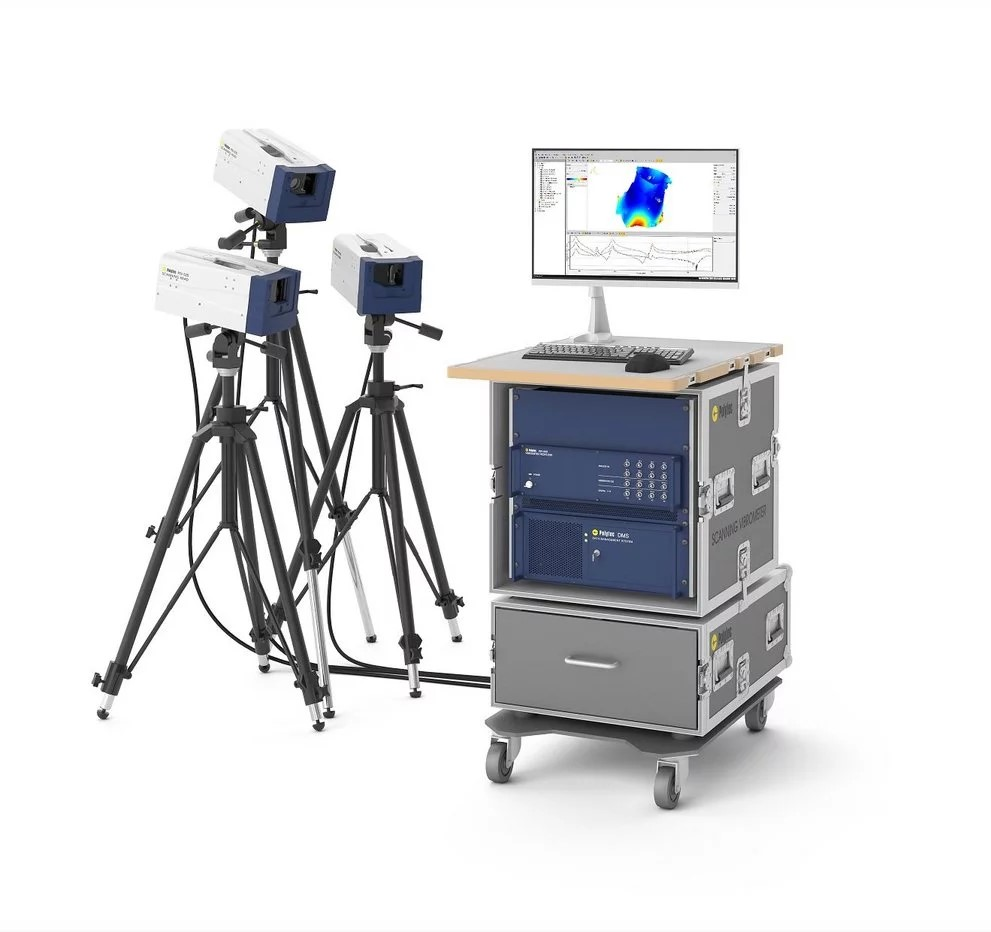
\includegraphics[width=0.6\textwidth]{img/ldv_3D.jpg}
\caption{System PSV-500-3D. Źródło: \cite{Polytec_LDV_3D}}
\label{img:ldv_3d}
\end{figure}

\subsection{Rozwiązanie zaproponowane w tej pracy}
Podstawowym problemem wibrometrii skanującej jest cena rozwiązania przedstawionego w \ref{cha:polytec_scan}. Cena zestawu trzech głowic skanujących jest bardzo wysoka.

Celem pracy jest skonstruowanie systemu, który pozwoliłby przeskanować powierzchnię, używając pojedynczej głowicy wibrometru punktowego. Można to osiągnąć na kilka różnych sposobów. Dwa rozważane na potrzeby tej pracy to:

\textbf{Ruchome lusterko} - Umieszczenie ruchomego lusterka przed wibrometrem, tak aby wiązka laserowa odbiła się od niego.

\textbf{Ruchomy wibrometr} - Umieszczenie całej głowicy wibrometru na stole, obracającym się dookoła osi $z$ oraz $y$, co pozwala celować całym wibrometrem w wybrany punkt na sferze dookoła wibrometru.

 W rozwiązaniu z obracającym się lusterkiem należałoby wziąć poprawkę na odbicie wiązki od lusterka. Odbicie takie wprowadza załamanie się wiązki i co za tym idzie, zmianę trasy wiązki laserowej. Wprowadza to wymóg przeprowadzanie skomplikowanych obliczeń na sygnale wyjściowym wibrometru. Rozwiązanie z lusterkiem wprowadziłoby także strefę martwą centralnie przed wibrometrem. Uniemożliwiłoby to pomiar punktów znajdujących się w tej strefie. Wymusiłoby natomiast pomiar punktów znajdujących się pod odpowiednim kątem do osi wibrometru.
 
 Ostatecznie zdecydowano się na wersję drugą, ruch całym wibrometrem. Jest to rozwiązanie koncepcyjnie prostsze ale wymaga mocniejszych silników i większego systemu pozycjonującego, co wprowadza inne wyzwania.
    \chapter{Projekt mechaniczny}
\label{cha:MechanicalDesign}
\section{Wibrometr}

\begin{figure}[h!] 
\centering 
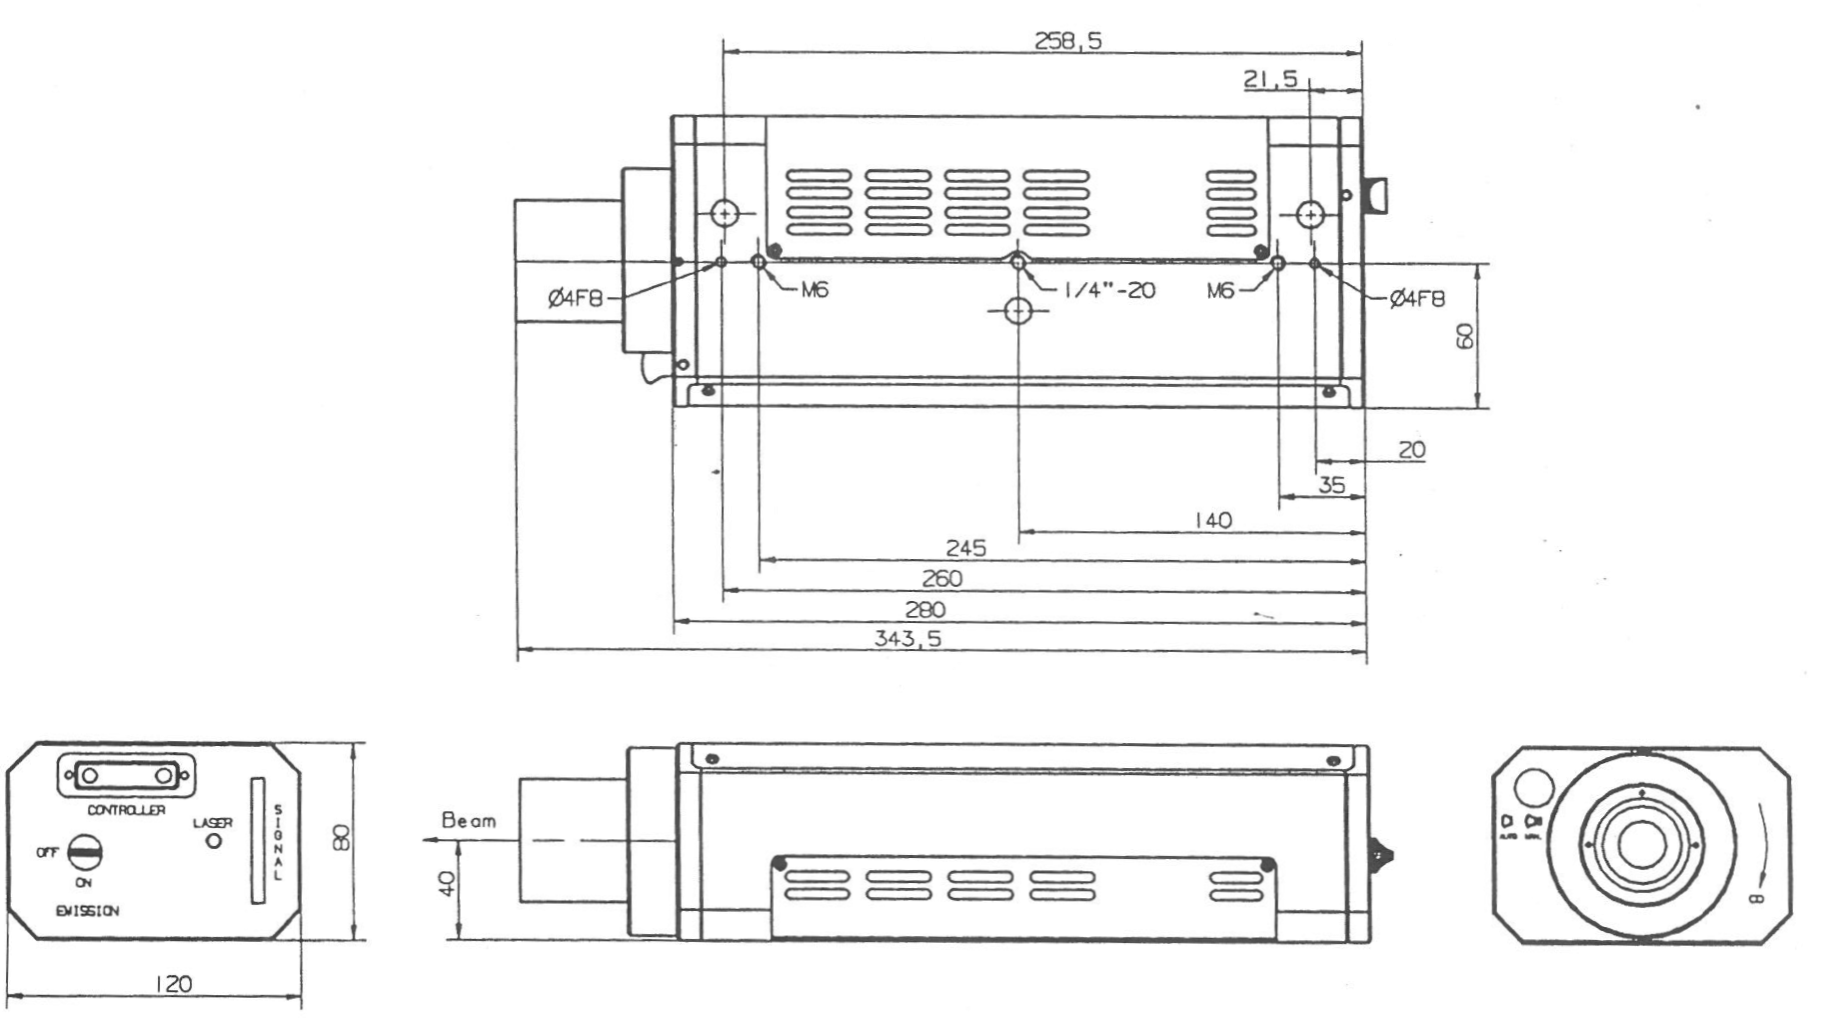
\includegraphics[width=0.8\textwidth]{img/wib_meas.png}
\caption{Wymiary głowicy OFV-353. Źródło: \cite{wib_docs} }
\label{img:wib_meas}
\end{figure}

Laboratorium Akustyki Technicznej (LAT) dysponuje wibrometrem wraz z głowicą OFV-353, i to pod tą głowicę projektowane będzie urządzenie. Można ją przybliżyć jako $3.5 kg$ prostopadłościan o wymiarach:
\vspace{-\topsep}
\begin{itemize}
    \item $280 mm$ wzdłuż osi $x$,
    \item $120 mm$ wzdłuż osi $y$,
    \item $80 mm$ wzdłuż osi $z$,
\end{itemize}
\vspace{-\topsep}
Zgodnie z rys. \ref{img:wib_meas}. \cite{wib_docs}
\subsection{Środek Masy}

Aby poprawnie poruszać wibrometrem, osie obrotów silników powinny obracać się w środku masy urządzenia. W przypadku systemów tak skomplikowanych jak wibrometr, najprostszą i najbardziej skuteczną metodą jest metoda doświadczalna. Próbując ustabilizować wibrometr w jednym punkcie, osiągnięto współrzędne środka masy. Jest to punkt odsunięty od środka geometrycznego o $\Delta_x = 1.5cm$. Gdzie oś $x$ to oś idąca wzdłuż dłuższego boku wibrometru razem z laserem wibrometru. W osi $y$ oraz $z$ środek masy jest zgodny ze środkiem geometrycznym. Biorąc poprawkę na gumowe podstawki wibrometru, środek masy jest odsunięty od ich spodu o $6cm$, co należy uwzględnić w modelu 3D.

\section{Jednostka napędowa}
\noindent Podczas projektowania stołu wzięto pod uwagę wiele różnych jednostek napędowych:
\subsection{Serwomechanizm modelarski}

\begin{figure}[h!] 
\centering 
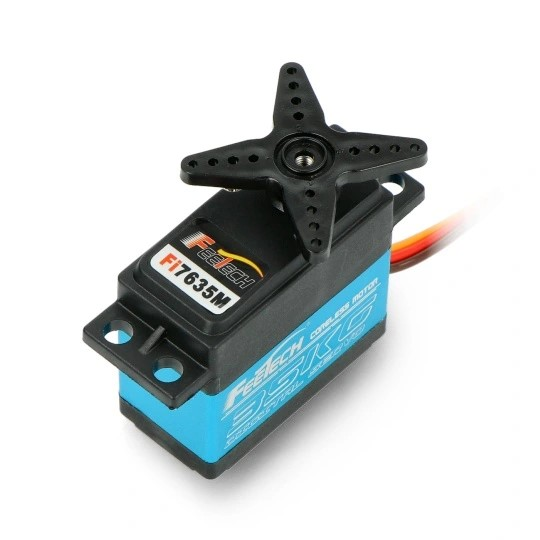
\includegraphics[width=0.5\textwidth]{img/feetech_servo.jpg}
\caption{Serwo Feetech FI7635M, przykładowe serwo modelarskie. Źródło: \cite{feetech_servo_docs}}
\label{img:feetech_servo}
\end{figure}

Pierwszym rozważanym typem jednostki napędowej był serwomechanizm modelarski (\textbf{standard servo}) (przykład na zdj. \ref{img:feetech_servo}). Serwa takie mają stosunkowo małe momenty obrotowe (sięgające do $35 kg \cdot cm$). Posiadają bardzo drobne, kruche przekładnie i z wielu wcześniejszych doświadczeń wynika, że nie są to trwałe rozwiązania. Problemem jest także zakres ruchu, który zwykle wynosi $+-180^{\circ}$. Serwo nie obróci się dalej niż pełne $360^{\circ}$, w środku znajduje się fizyczna blokada. (Wyjątkiem są serwa typu $360^{\circ}$, jednakże serwa te pozwalają na kontrolę prędkości obrotowej, nie pozycji.) Plusami serw modelarskich jest prostota obsługi. Pozycja jest proporcjonalna do wartości wypełnienia PWM sygnału podanego na pin sygnałowy serwomechanizmu, Dodatkowo posiadają one wbudowany enkoder absolutny, co powoduje że nawet po odcięciu zasilania serwo pamięta swoją pozycję. Jednakże ten typ jednostki napędowej został odrzucony, jako rozwiązanie nieadekwatne do tego zastosowania. Serwomechanizmy są zbyt małe, aby obsłużyć omawiany wibrometr. \cite{feetech_servo_docs}


\subsection{Silnik krokowy}
Kolejnym rozwiązaniem jakie sprawdziłoby się w takim zastosowaniu to silniki krokowe (\textbf{stepper motor}) (przykład na zdj. \ref{img:stepper}). Są one także bardzo proste do wysterowania. W zależności od podtypu silnika sterowanie różni się, ale zasada jest zawsze ta sama - należy jedynie podawać informacje o kolejnych krokach na sterownik, który obraca silnik o znany kąt, odpowiadający jednemu krokowi. Posiadają one jednak dużo niższe momenty obrotowe niż inne rozwiązania, a przekładnie zmniejszające prędkość a zwiększające moment są stosowane, ale raczej rzadko. A na pewno nie tak często jak z innymi jednostkami napędowymi. \cite{pololu_steppers}

\begin{figure}[h!] 
\centering 
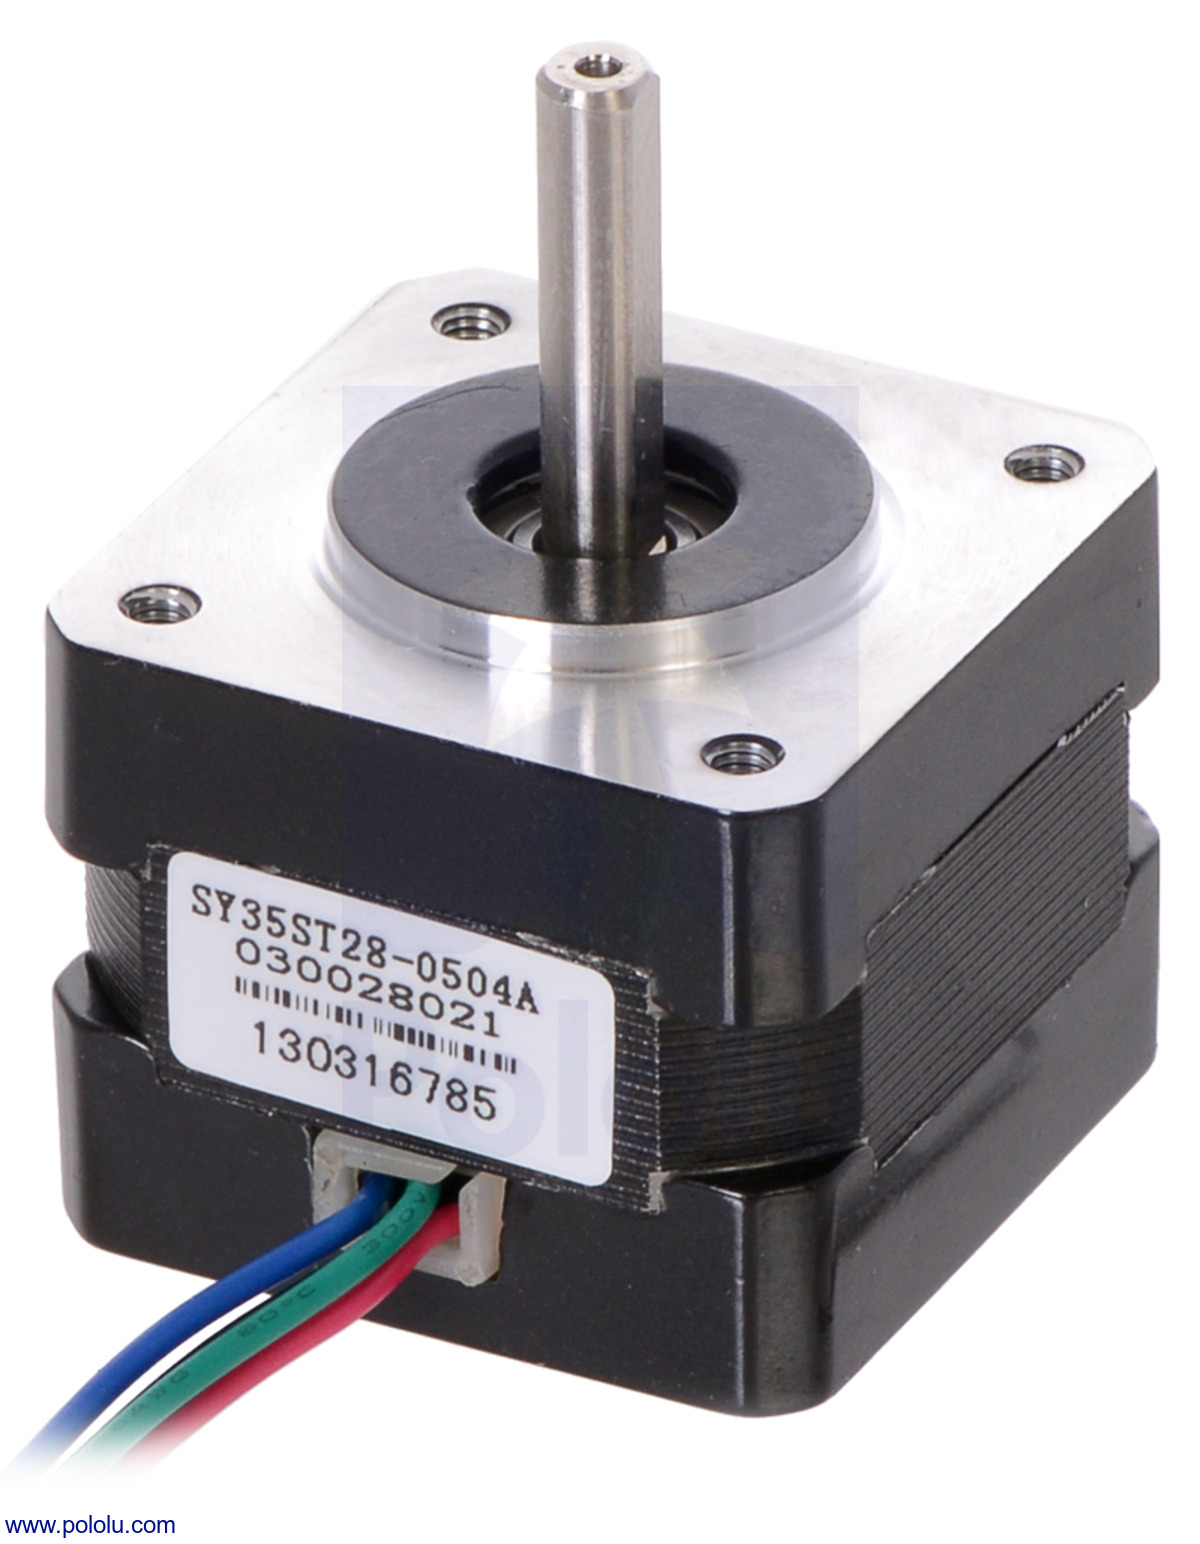
\includegraphics[width=0.4\textwidth]{img/stepper.jpg}
\caption{Silnik krokowy bipolarny, model Pololu 1208. Źródło: \cite{pololu_steppers}}
\label{img:stepper}
\end{figure}

Silniki mogą mieć różną precyzję, ale najczęściej spotykane są wartości rzędu od 100 do 400 kroków na obrót, co daje precyzję około $3.6^{\circ} - 0.9^{\circ}$, co może być za mało jak na ten projekt. \cite{motrioncontrol_stepper_guide} Precyzje potrafią sięgać aż do 1000 kroków na obrót przy droższych liniach silników, jednakże nie są one aż tak popularne jak wartości z rzędu setek kroków na obrót. \cite{pololu_stepper_forum}

Dodatkowo silniki krokowe mają duży pobór mocy, ponieważ nawet nieruchome pobierają prąd. Ostatecznie, przy silnikach krokowych zawsze istnieje ryzyko zgubienia kroku. Dlatego, jeżeli wymogiem jest znajomość pozycji z dużą dozą pewności, należałoby zastosować dodatkowy enkoder, który niezależnie sprawdzi czy nie nastąpiło zgubienie kroku.

Ostatecznie, silnik krokowy po dodaniu przekładni i dodatkowego enkodera byłby dobrym rozwiązaniem. Jednakże z powodu rozmiarów, i co za tym idzie bezwładności oraz wymaganego momentu, a także z powodu małej popularności gotowych rozwiązań łączących silnik krokowy, przekładnię oraz enkoder, pomysł zastosowania silnika krokowego został porzucony.

\subsection{Silnik szczotkowy prądu stałego}
\label{cha:brushed_dc_motor}
Ostatecznie najlepszym kandydatem okazał się być klasyczny silnik szczotkowy prądu stałego (\textbf{Brushed DC Motor}). Silniki te posiadają stosunkowo małe wymiary. Ponadto dołączenie przekładni daje bardzo duże momenty obrotowe, a zastosowanie enkodera daje realne sprzężenie zwrotne, mówiące o ruchu silnika. Poważnym utrudnieniem jest sposób ich sterowania. Nie są to silniki naturalnie przystosowane do kontroli pozycji. Pozycję należy odczytać z enkodera i na silnik podać sterowanie, odpowiadające prędkości obrotu silnika, które doprowadzi wał do pozycji docelowej. Jest to jednak utrudnienie, które jeżeli zostanie pokonane, da najlepsze rezultaty. Do projektu został wybrany silnik z linii Pololu 37D. Są to silniki z zamontowaną przekładnią, oraz w zależności od modelu, mają także enkoder. Jako że w projekcie tym priorytetem jest uciąg silnika, a nie prędkość kątowa wału, zdecydowano się na największą możliwą przekładnię, $150:1$. Dodatkowo wymogiem jest kontrola pozycji, dlatego wymagany jest wariant z enkoderem.

\begin{figure}[h!] 
\centering 
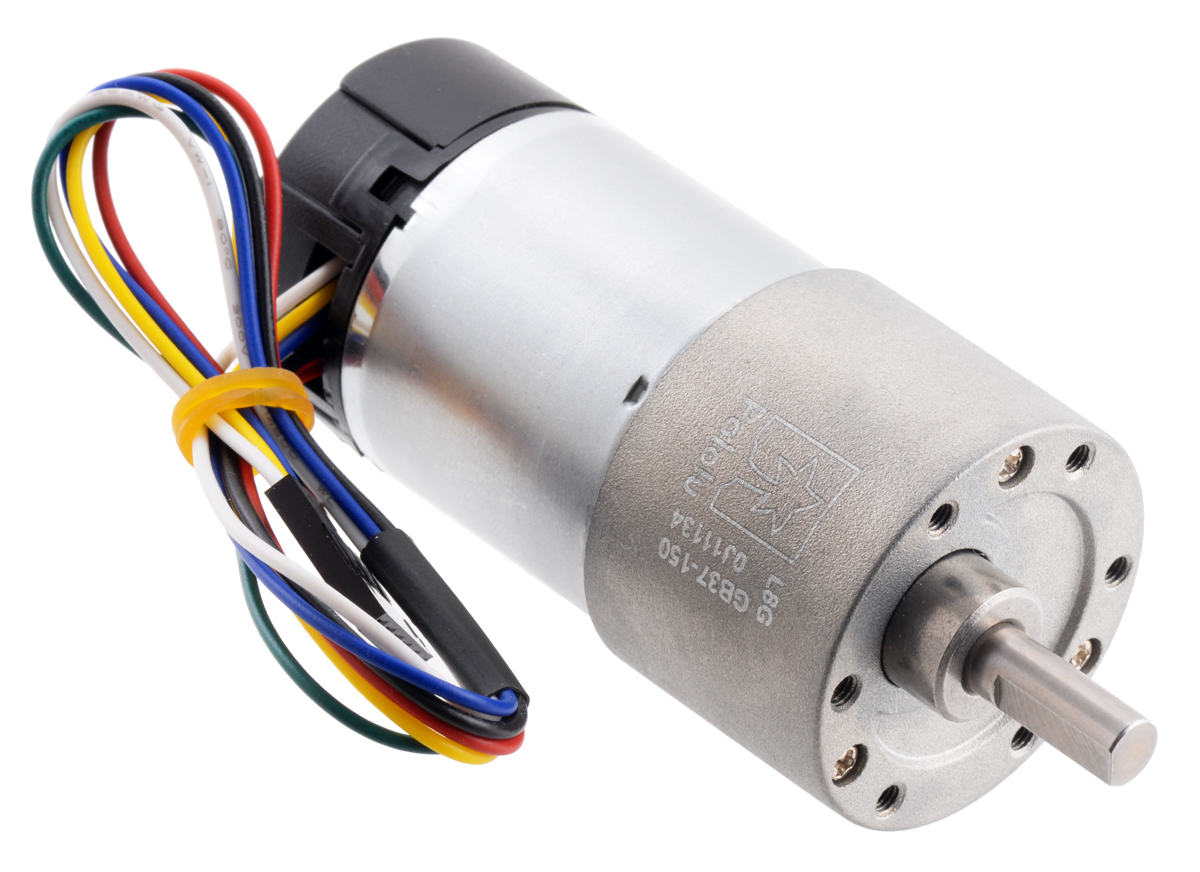
\includegraphics[width=0.4\textwidth]{img/pololu_2828.jpg}
\caption{Silnik szczotkowy prądu stałego Pololu 2828. Źródło: \cite{pololu_2828}}
\label{img:pololu2828}
\end{figure}

\noindent Po spełnieniu tych wszystkich kryteriów otrzymano silnik Pololu 2828 (przedstawionego na zdj \ref{img:pololu2828}), który \cite{pololu_2828}: 
\vspace{-\topsep}
\begin{itemize}
    \item Jest zasilany napięciem 12V
    \item Posiada prędkość obrotową bez obciążenia wynoszącą $67RPM$
    \item Moment obrotowy równy $49 kg \cdot cm$
    \item Bez obciążenia pobiera jedynie $200mA$
    \item Pod maksymalnym obciążeniem pobiera nawet do $5.5A$
    \item Posiada wbudowany enkoder o rozdzielczości $64CPR$, co po uwzględnieniu przekładni daje $9600CPR$.
\end{itemize}

\section{Modele 3D}
\subsection{Projekt}
Układ pozycjonujący wibrometr został zaprojektowany w układzie współrzędnych kątowych RPY, czyli kątów \textbf{Roll}, \textbf{Pitch}, \textbf{Yaw}, przedstawionych na rys. \ref{img:RPY}. Jak widać, oś obrót dookoła osi roll odpowiada obrotowi dookoła osi $x$, oś yaw odpowiada osi $z$ a oś pitch odpowiada osi $y$. 

\begin{figure}[h!] 
\centering 
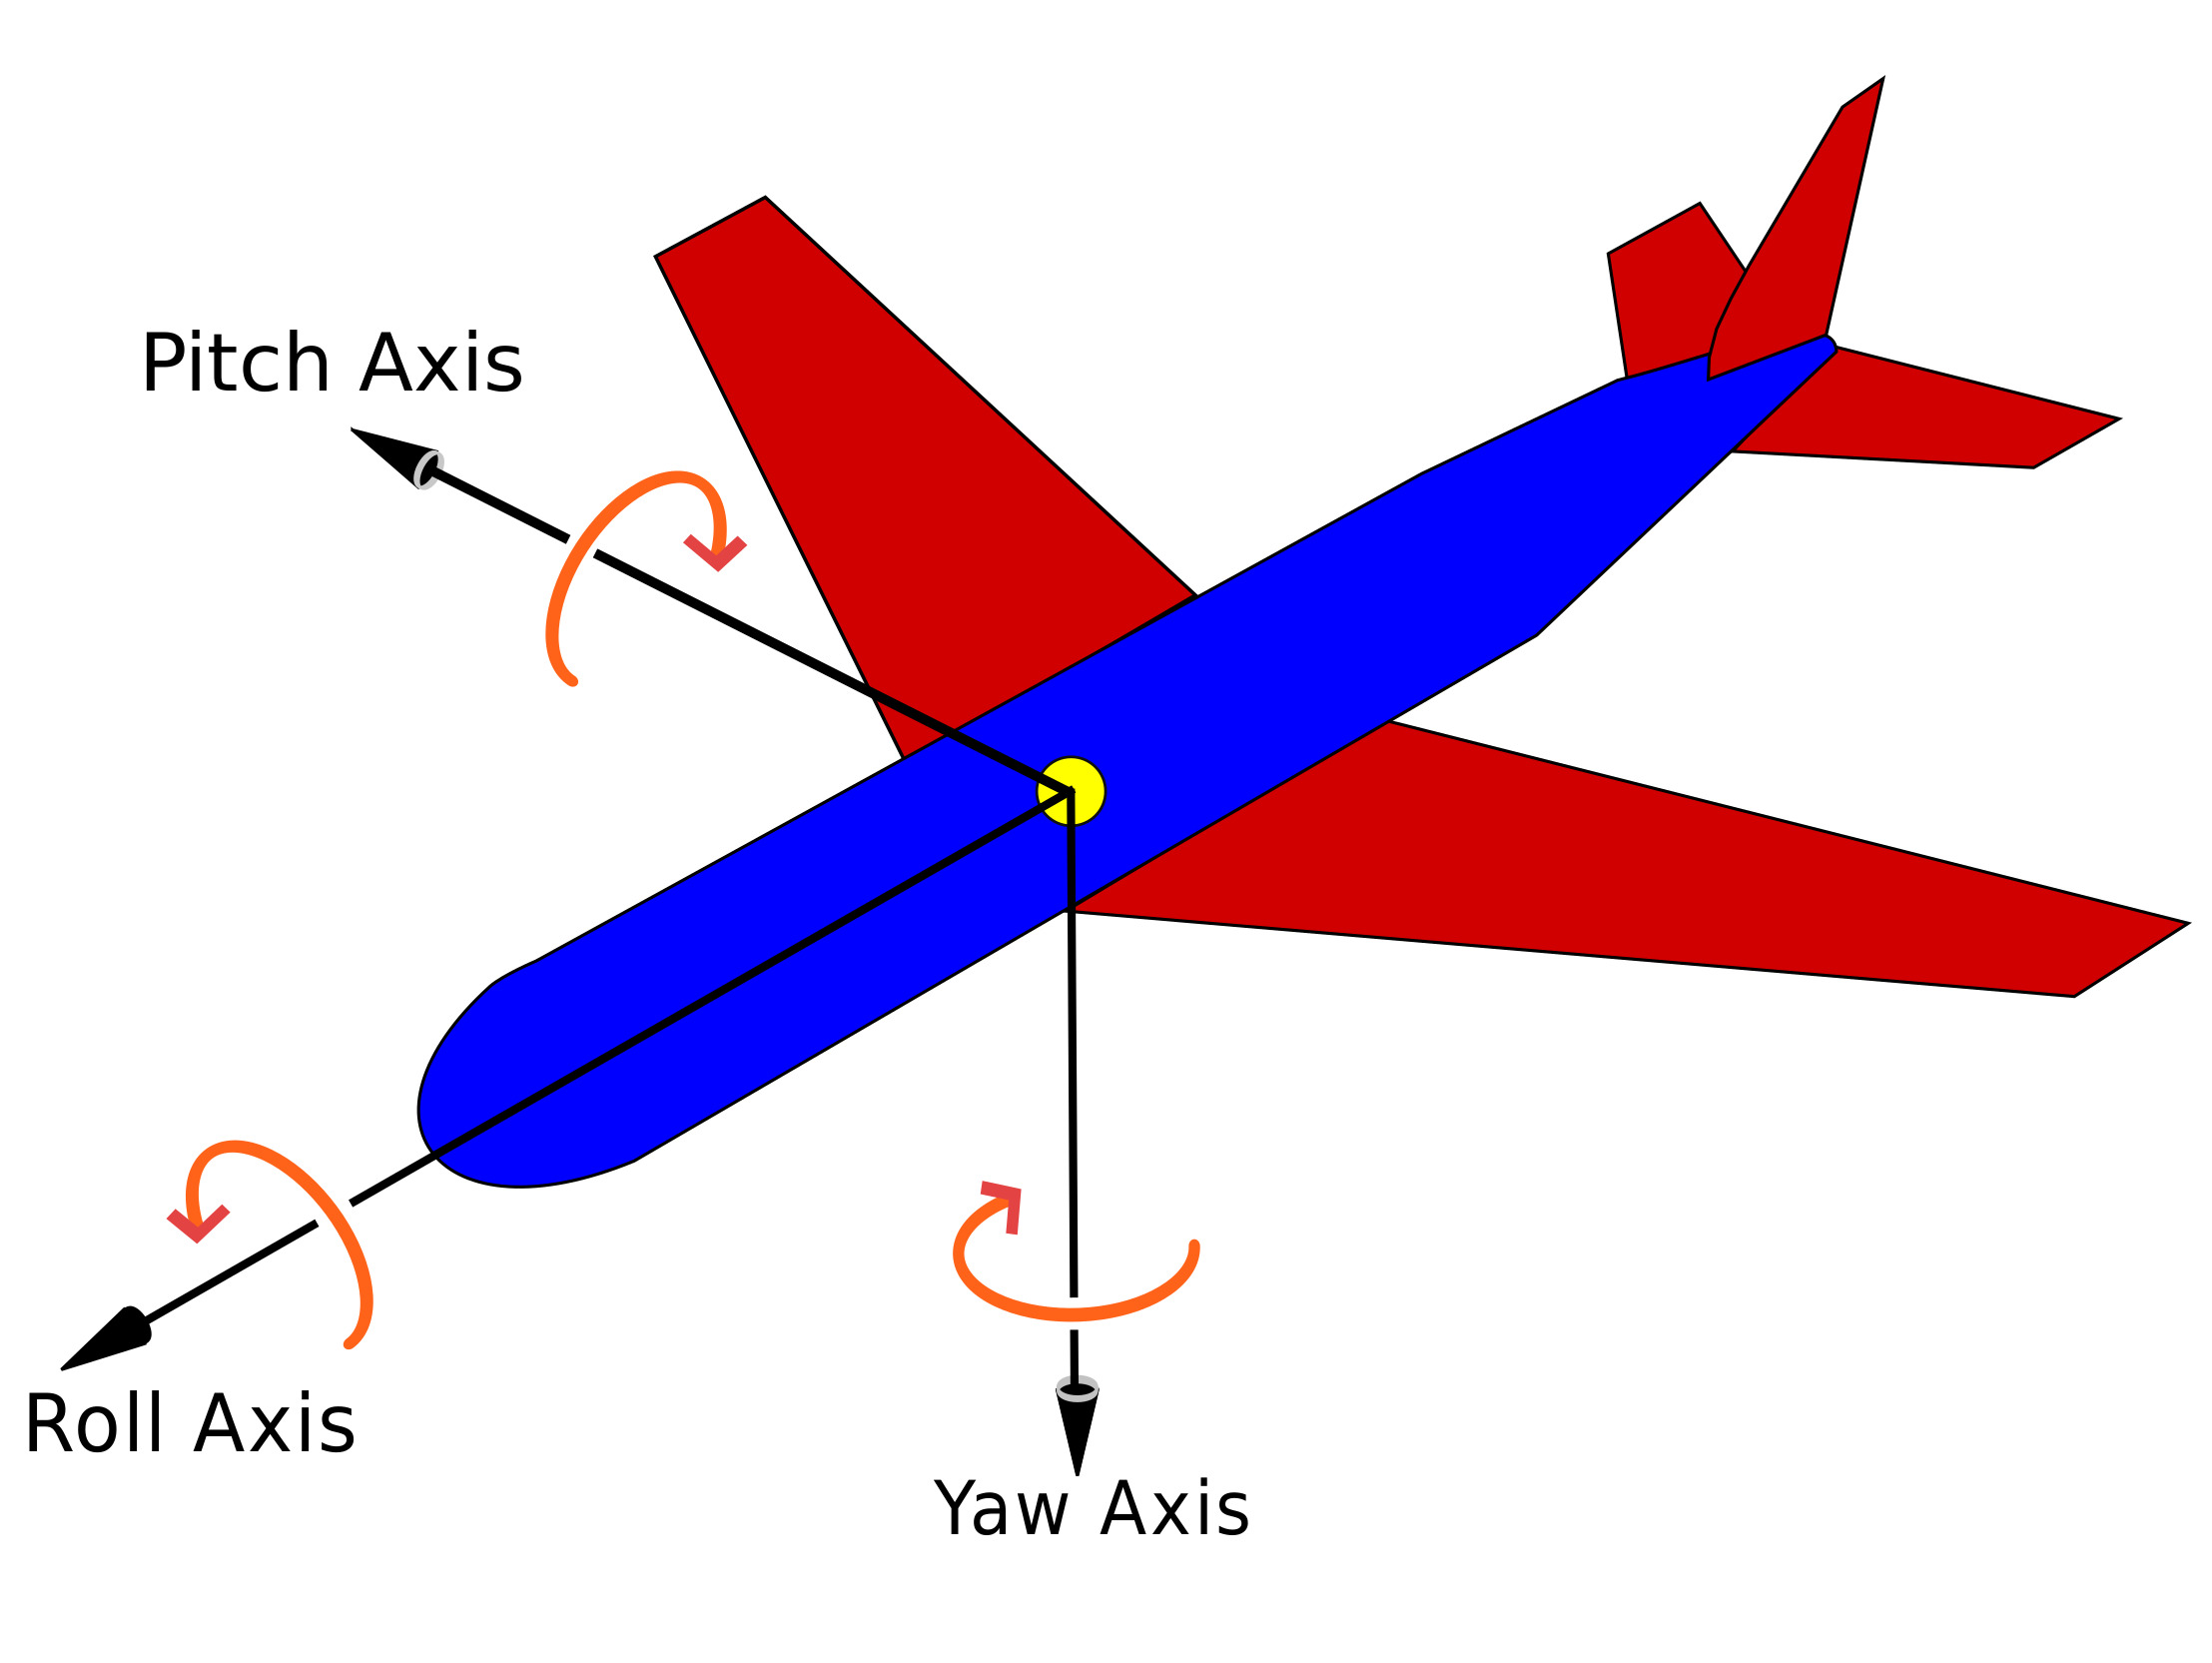
\includegraphics[width=0.6\textwidth]{img/RPY.jpg}
\caption{Osie RPY. Źródło: \cite{RPY_obrazek}}
\label{img:RPY}
\end{figure}

Celem pracy jest zaprojektowanie stołu, który obróci wibrometr dookoła osi yaw i pitch, natomiast laser wibrometru będzie poruszał się wzdłuż osi roll, która pozostaje nieruchoma.

\subsection{Wykonanie modeli}
\label{cha:3d_models_assembly}
Modele zostały wykonane w oprogramowaniu Autodesk Fusion 360. Jest to chmurowe oprogramowanie typu 3D CAD, pozwalająca na tworzenie modeli oraz całych złożeń. Zostało ono wybrane ze względu na opcje łatwego przechowywania modeli w chmurze, co pozwala na wygodną pracę na wielu komputerach na raz. \cite{Fusion_opis}

\begin{figure}[h!] 
\centering 
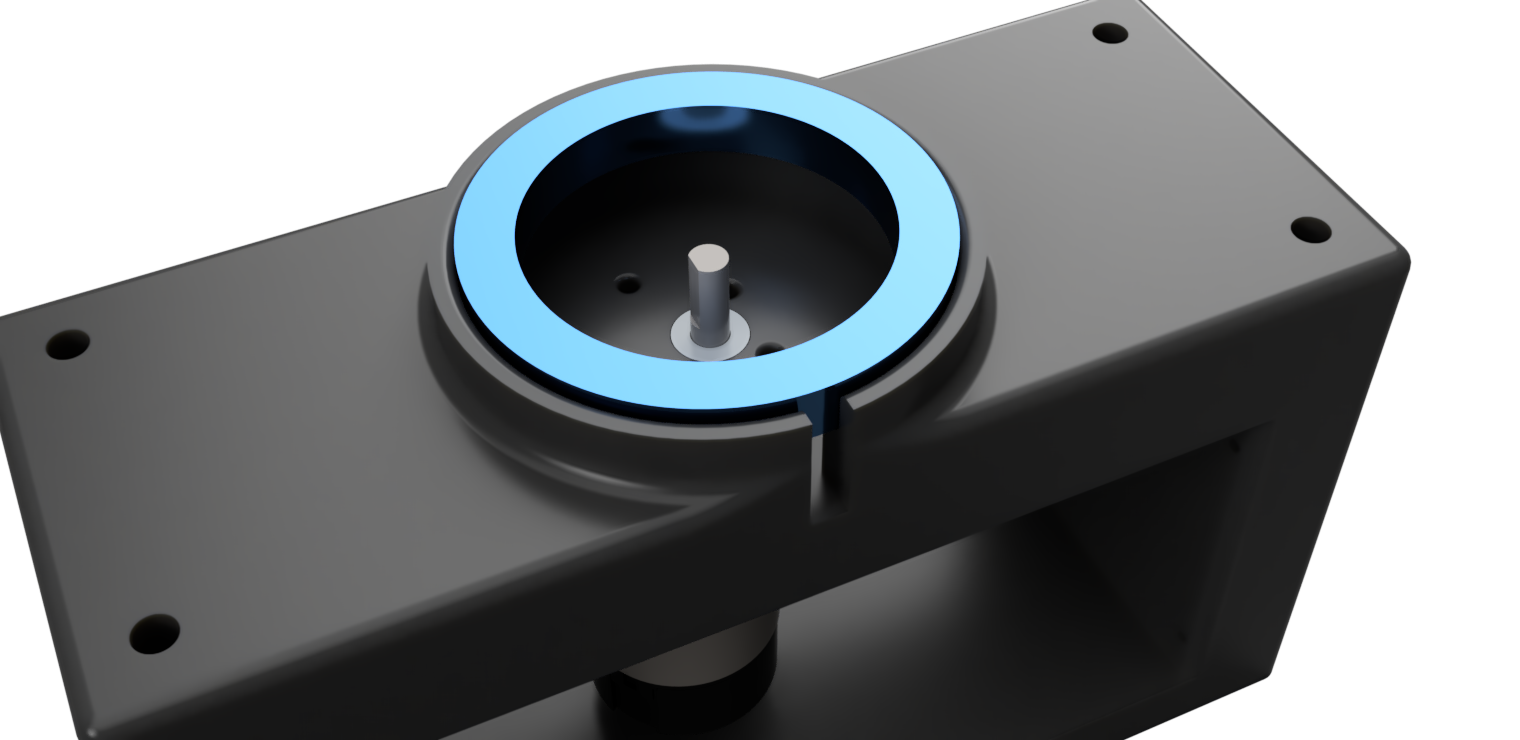
\includegraphics[width=0.6\textwidth]{img/Fusion1.png}
\caption{Złożenie części statycznej stołu oraz pierwszego silnika.}
\label{img:fusion_1}
\end{figure}

W pierwszej kolejności zostało opracowane połączenie między dolnym silnikiem, obracającym się dookoła osi yaw (z), a częścią stołu, która także ma się dookoła tej osi obracać. Na rys. \ref{img:fusion_1} można zauważyć, że statyczna część tego silnika jest przymocowana do statycznej części stołu. Na niej, dookoła wału, leży łożysko kulkowe o wymiarze $55x72x9mm$ (na \ref{img:fusion_1} zaznaczone niebieskim kolorem). Łożysko zostało zastosowane aby nie opierać masy wibrometru bezpośrednio na wale silnika. Kolejny krok, przedstawiony na rys. \ref{img:fusion_2}, prezentuje montaż wału do obrotowej części stołu. Wspomniana część jest przymocowana do wału poprzez gotowy hub montażowy Pololu 1083 (przedstawiony na rys \ref{img:pololu_hub}) oraz kilka dystansów, pozwalających odsunąć środkową, obrotową część stołu od wału silnika.

\begin{figure}[h!] 
\centering 
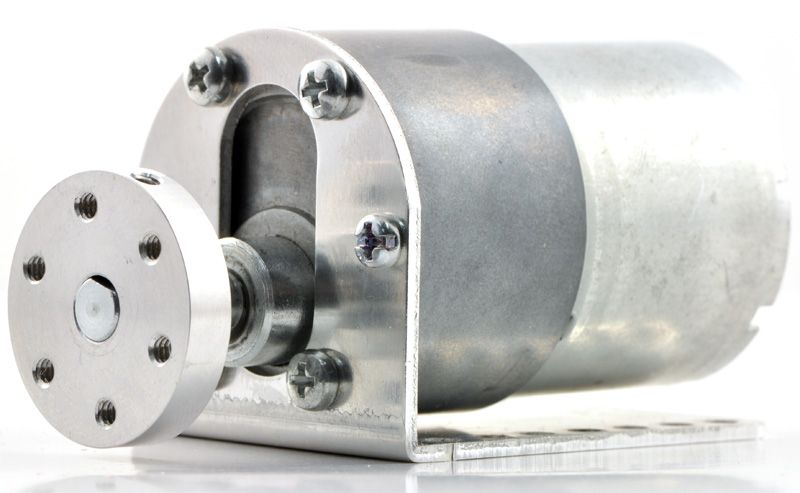
\includegraphics[width=0.3\textwidth]{img/pololu_hub.jpg}
\caption{Pololu Hub na wał 6mm (Pololu 1083). Źródło: \cite{Pololu_hub}}
\label{img:pololu_hub}
\end{figure}

Dodatkowo na obu rysunkach można zaobserwować, że środkowa, obrotowa część stołu jest umieszczona wewnątrz wspomnianego łożyska, leży na wewnętrznym jego pierścieniu. Natomiast dolna, statyczna część stołu znajduje się na zewnątrz łożyska. Łożysko spoczywa swoim zewnętrznym pierścieniem na statycznej części stołu. Dodatkowo rys. \ref{img:fusion_1} przedstawia otwór, pozwalający przykręcić wspomniany wcześniej hub do wału silnika.


\begin{figure}[h!] 
\centering 
\begin{subfigure}{.4\textwidth}
  \centering
  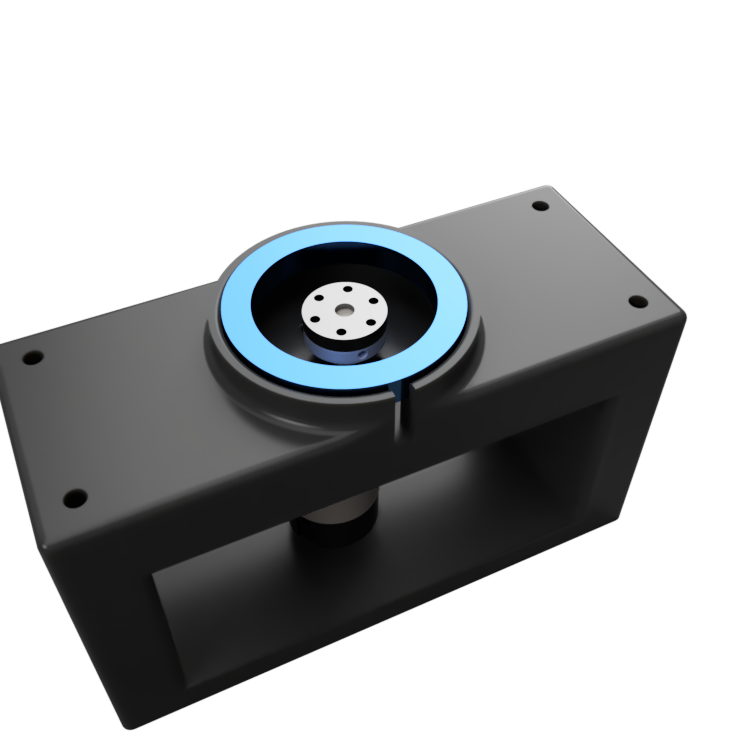
\includegraphics[width=\textwidth]{img/Fusion2a.png}
\end{subfigure}%
\begin{subfigure}{.4\textwidth}
  \centering
  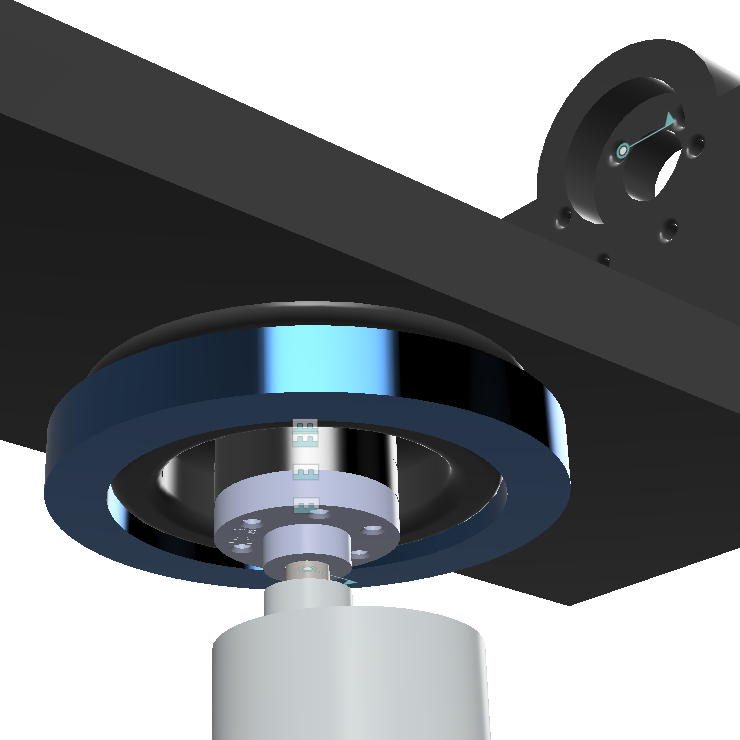
\includegraphics[width=\textwidth]{img/Fusion2b.png}
\end{subfigure}
\caption{Montaż wału silnika do środkowej części obrotowej.}
\label{img:fusion_2}
\end{figure}

Kolejnym krokiem było przymocowanie drugiego silnika do środkowej, obrotowej części, tak aby nadać konstrukcji drugą oś swobody. Montaż samego silnika jest przedstawiony na rys. \ref{img:fusion_3a}. Na wał silnika także został zamontowany hub mocujący, który, aby odciążyć sam wał, został wsunięty w łożysko, które w tym miejscu ma wymiary $12x28x8mm$ (Zaznaczone na rys. \ref{img:fusion_3b} kolorem czerwonym). Do huba przymocowana jest część tzw. Holder, która ma podtrzymywać wibrometr. Ma ona już obie osie swobody, potrafi się obracać dookoła osi yaw dzięki pierwszemu silnikowi, jak i dookoła osi pitch dzięki drugiemu silnikowi. Symetrycznie, naprzeciwko silnika drugiego, także znajduje się otwór pod łożysko. Jednakże w tym miejscu nie montujemy silnika, a zamiast niego Holder podobny do tego montowanego do huba. Opisywany, drugi Holder, zamiast otworów montażowych do huba, posiada własny wał wkładany w łożysko. Montaż tych dwóch części widoczny jest na rys. \ref{img:fusion_4}.

\begin{figure}[h!] 
\centering 
\begin{subfigure}{.6\textwidth}
\centering 
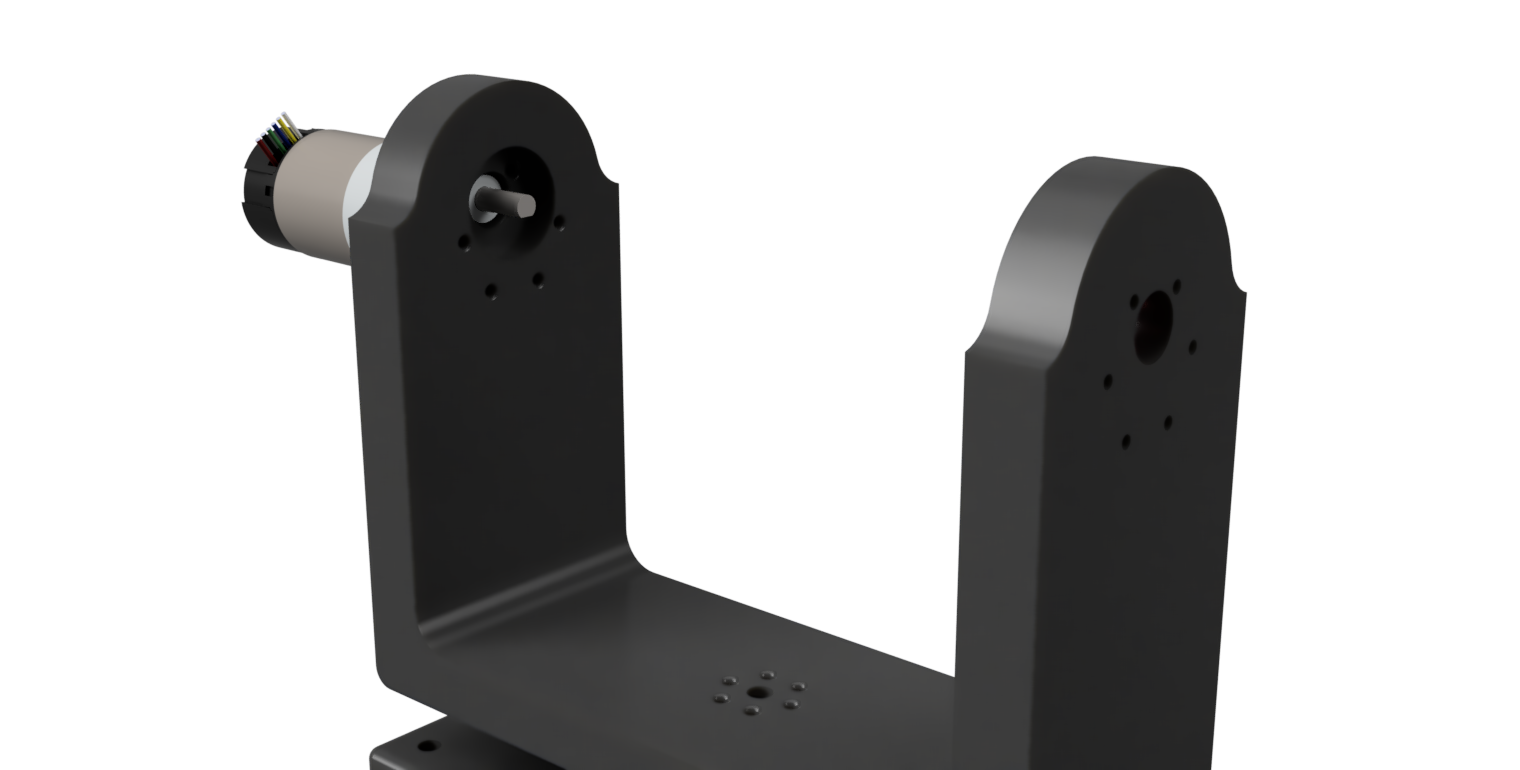
\includegraphics[width=\textwidth]{img/Fusion3a.png}
\caption{Montaż drugiego silnika do części ruchomej obrotowej}
\label{img:fusion_3a}
\end{subfigure}%
\begin{subfigure}{.4\textwidth}
\centering 
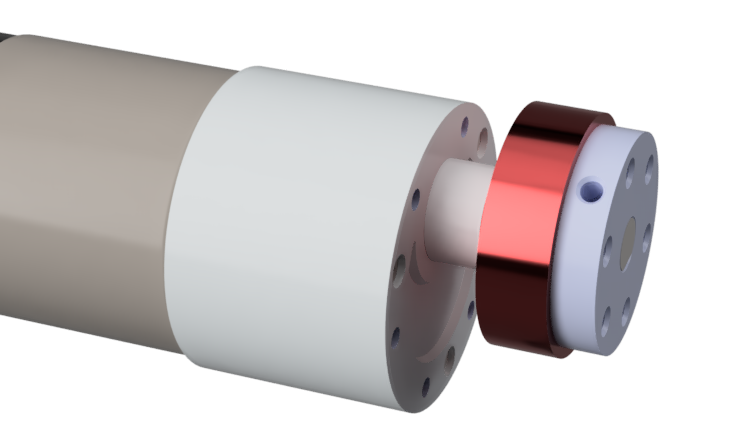
\includegraphics[width=\textwidth]{img/Fusion3b.png}
\caption{Montaż łożyska oraz hub-a montażowego do drugiego silnika}
\label{img:fusion_3b}
\end{subfigure}
\label{img:fusion_3}
\caption{Montaż drugiego silnika.}
\end{figure}

\begin{figure}[h!] 
\centering 
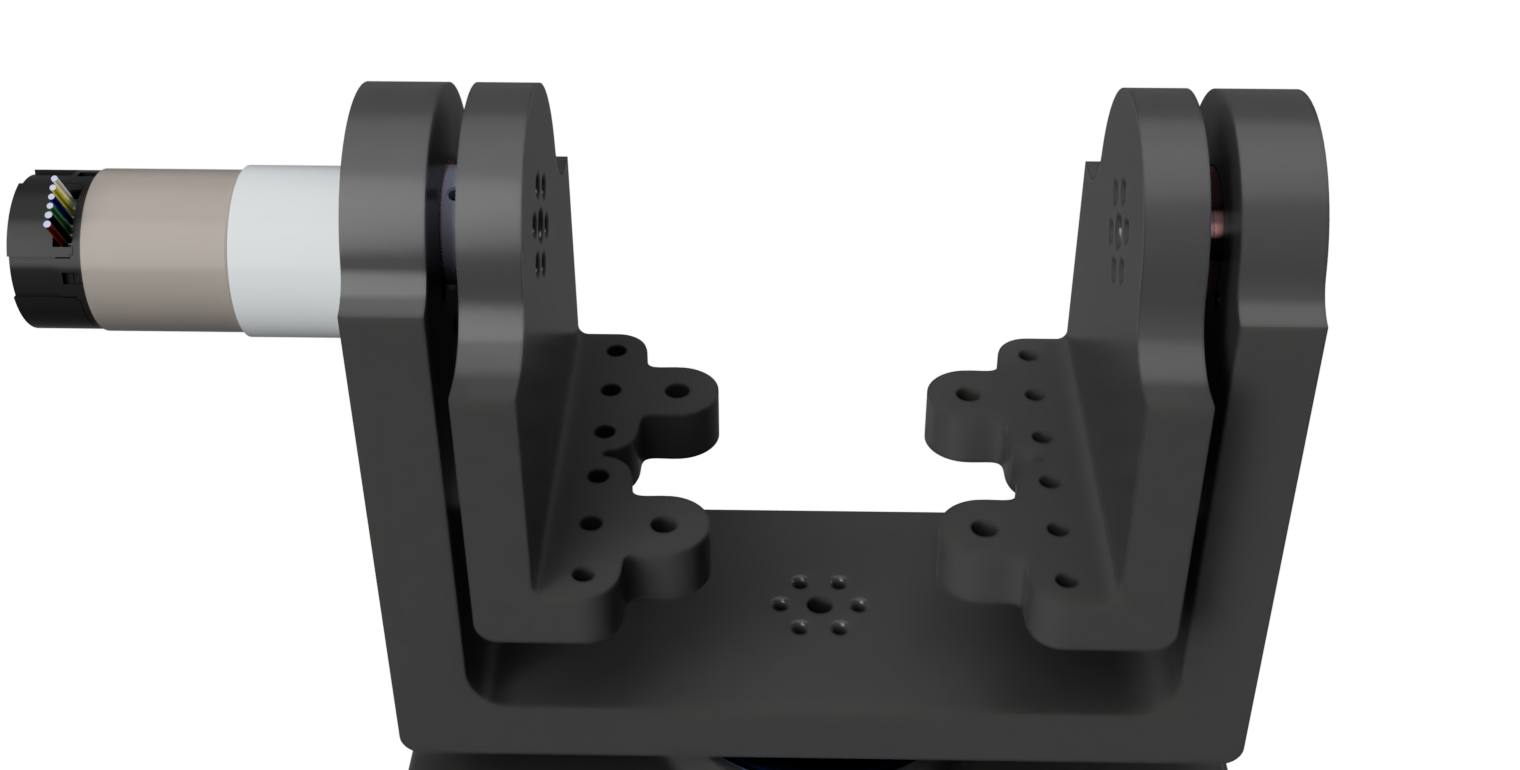
\includegraphics[width=0.7\textwidth]{img/Fusion4.png}
\caption{Montaż obu holderów do reszty modelu.}
\label{img:fusion_4}
\end{figure}

Oba holdery podtrzymują płytę, do której przykręcany jest wibrometr. Obrazuje to rys. \ref{img:fusion_5}, który przedstawia całość stołu pozycjonującego wibrometr dookoła osi yaw oraz pitch w układzie współrzędnych RPY.

\begin{figure}[h!] 
\centering 
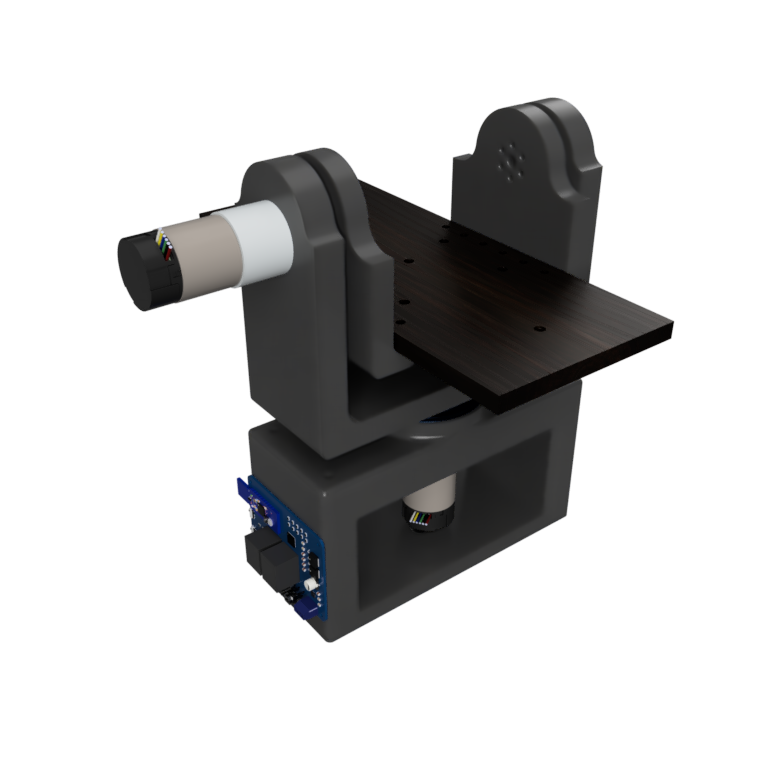
\includegraphics[width=1\textwidth]{img/Fusion5.png}
\caption{Model całej złożonej konstrukcji.}
\label{img:fusion_5}
\end{figure}

    \chapter{Układ elektroniczny}
\label{cha:Electronics}
Układ elektroniczny na potrzeby projektu został uproszczony do minimum. Składa się z układu zasilającego, zapewniającego napięcie $12V$ oraz prąd $5A$, oraz gotowej płytki sterownika do silników szczotkowych, do której podpięte są 2 silniki. Dodatkowo płytka jest połączona z komputerem za pomocą kabla USB.

\section{Płytka Nrf Dongle Brushed Motor Controller}

\begin{figure}[h!] 
\centering 
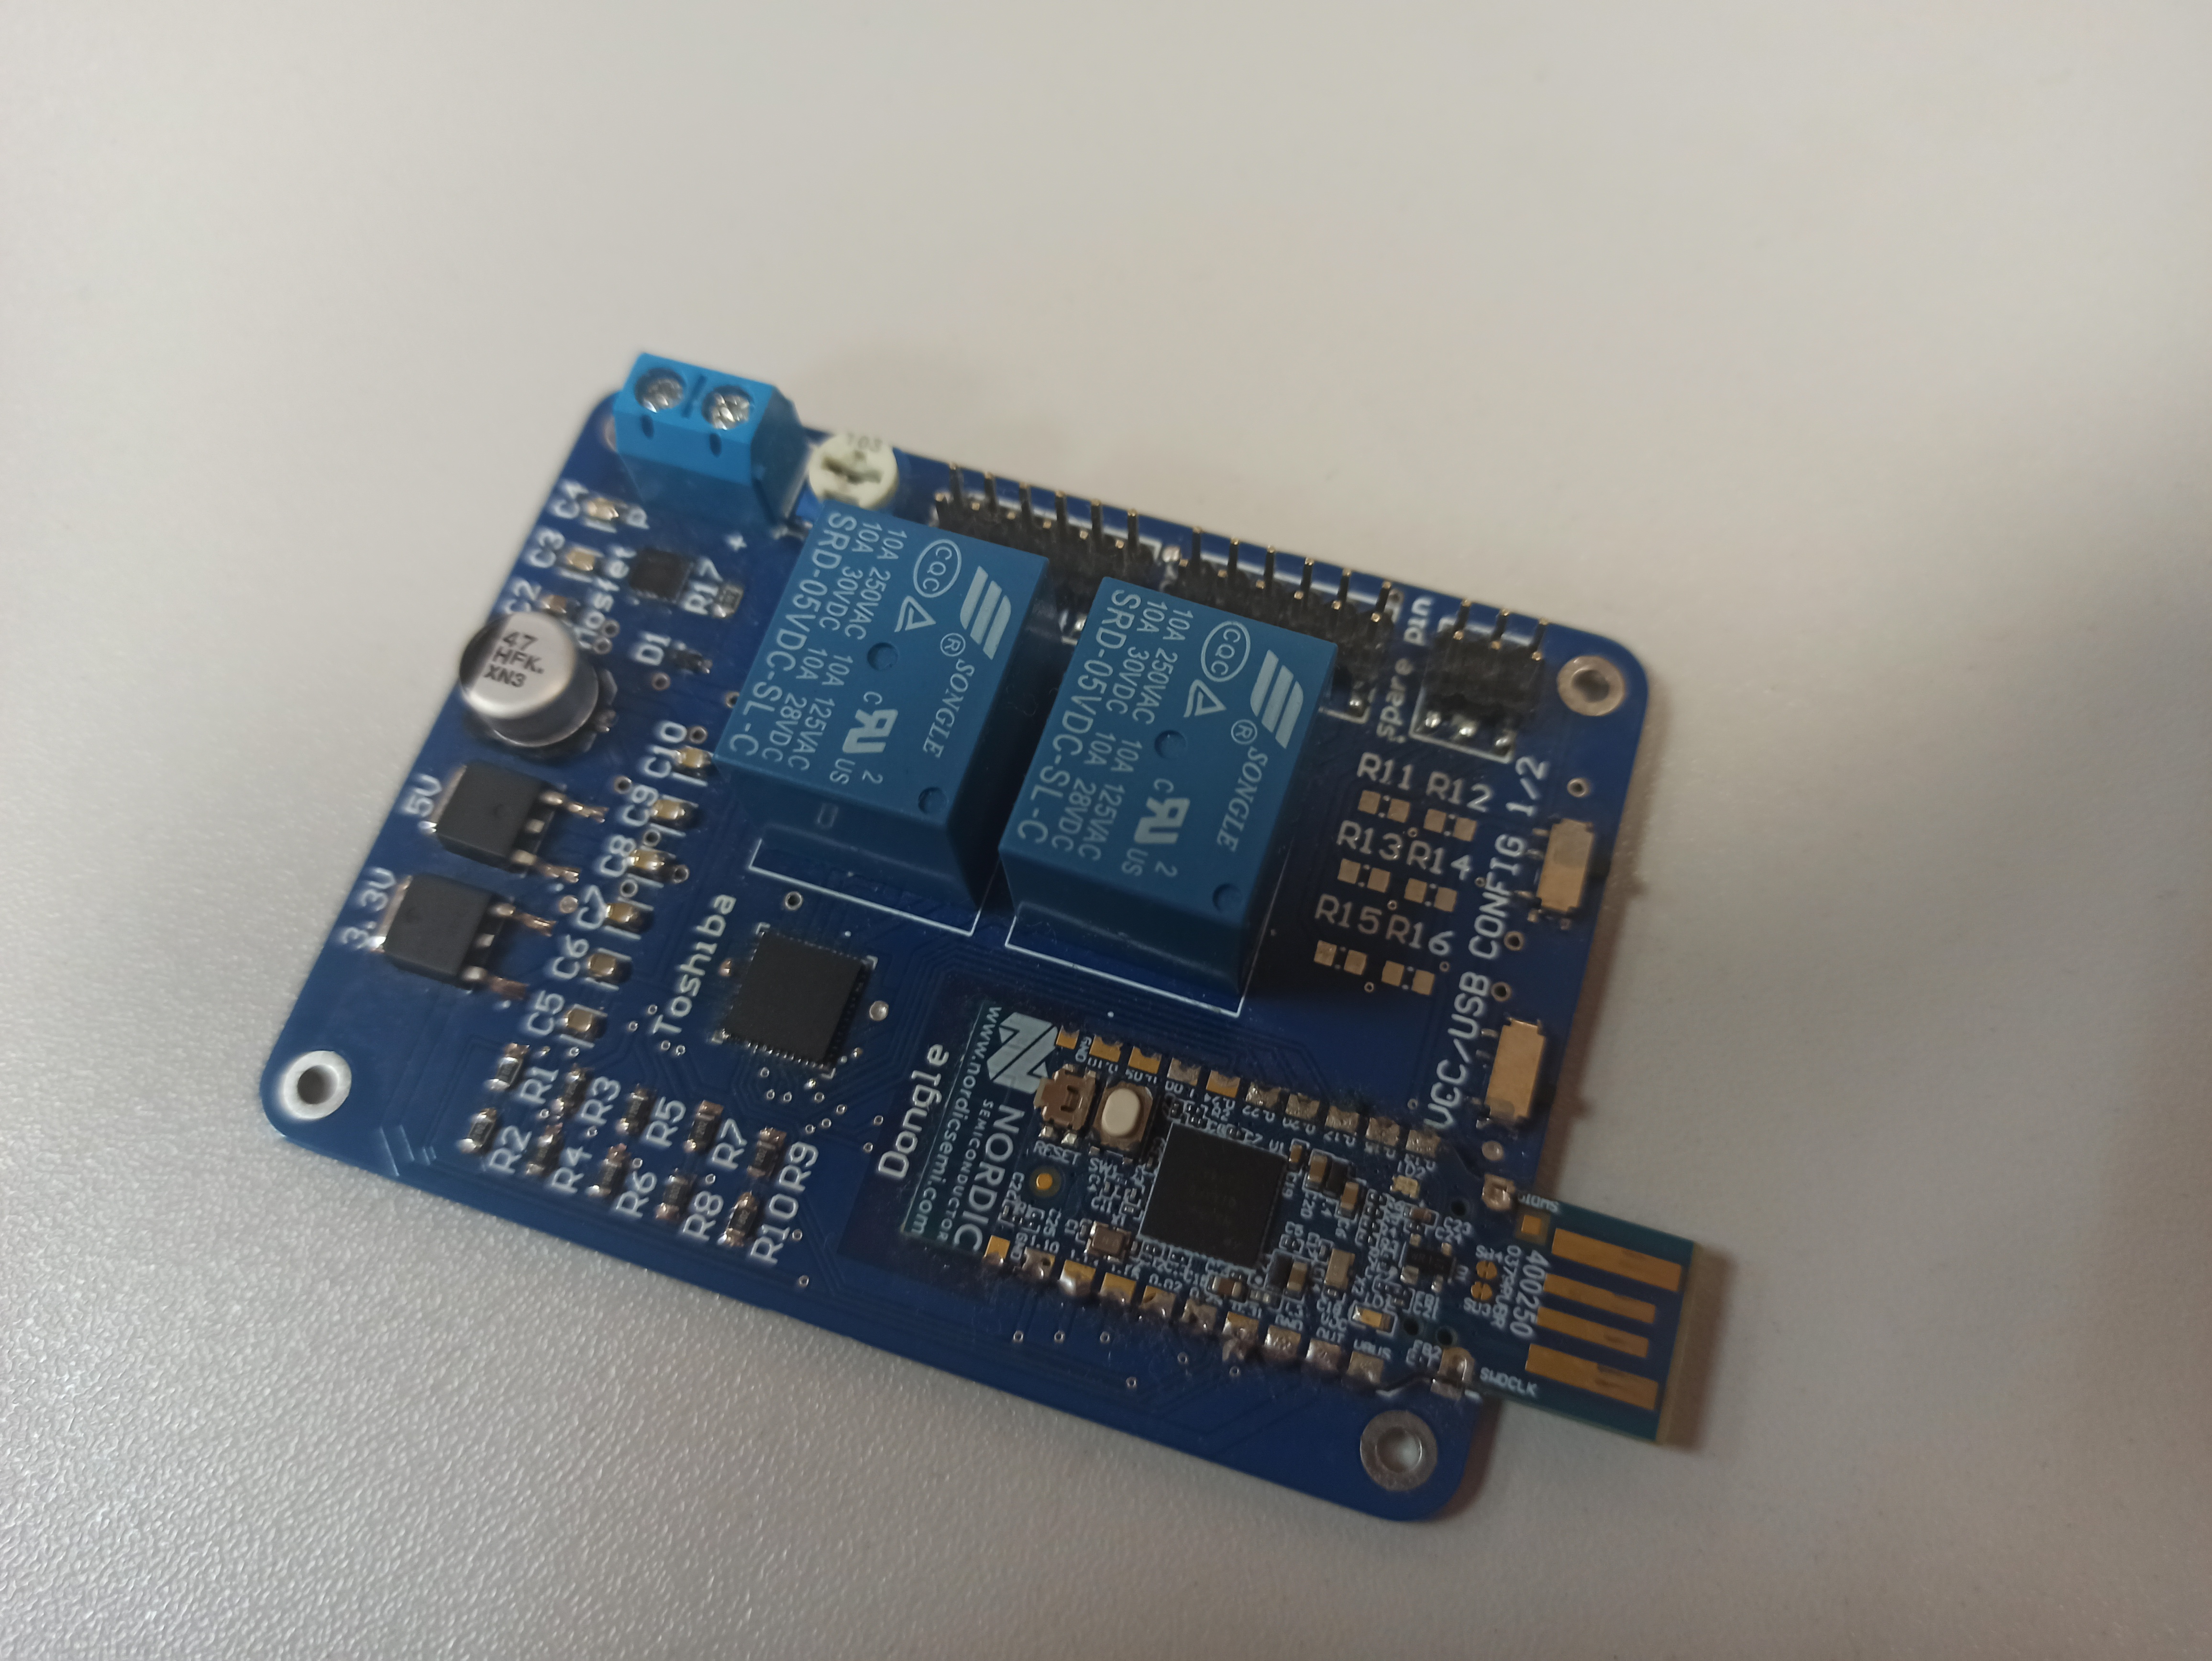
\includegraphics[width=0.8\textwidth]{img/PcbPhoto.jpg}
\caption{Zdjęcie sterownika do silników. Źródło: \cite{nrf_mc_hw}}
\label{img:full_pcb}
\end{figure}

Płytka Nrf Dongle Brushed Motor Controller to układ (przedstawiony na rys. \ref{img:full_pcb}) typu development kit/evaluation board wykonany w kole naukowym "Integra". Układ przede wszystkim składa się z nRF52840 Dongle - płytki prototypowej od firmy Nordic Semiconductors. Procesor nRF52840  kontroluje układ scalony Toshiba TB67H420FTG, który jest dwukanałowym sterownikiem do silników szczotkowych prądu stałego. Na płytce dodatkowo znajdują się 2 układy LDO, które zmniejszają napięcie zasilania z $12V$ do kolejno $5V$ oraz $3.3V$. Linia zasilająca $3.3V$ używana jest do zasilenia mikrokontrolera nRF52840, który jest zasilany napięciem $1.7V$ - $5.5V$. Linia zasilająca $5V$ jest natomiast używana do zasilenia enkodera, który w przypadku silników Pololu 2828 może być zasilany dowolnym napięciem z zakresu $3.5V$ do $20V$. Dodatkowo linie zasilające wyprowadzone są na piny zewnętrzne, aby można było zasilić potencjalne peryferia. Na płytce znajduje się także przeprowadzenie wolnych pinów GPIO (\textbf{General-purpose input/output}, Piny typu Wejście-wyjście ogólnego przeznaczenia) z procesora, oraz przede wszystkim dwa komplety pinów obsługujących silniki z odpowiadającymi im enkoderami. Opisy pinów znajdują się na rewersie płytki.\cite{nrf_mc_hw}



\subsection{nRF52840 Dongle}
\textbf{nRF52840 Dongle} (zdj. \ref{img:full_pcb}) to płytka prototypowa z mikrokontrolerem nRF52840 na pokładzie. Jest programowalna po USB, wspiera większość współczesnych protokołów IoT, jak Bluetooth 5.4, Thread czy Zigbee. Posiada też programowalne 2 diody, przycisk, jak i 15 wyprowadzeń typu GPIO. \cite{nrf_dongle}

\begin{figure}[h!] 
\centering 
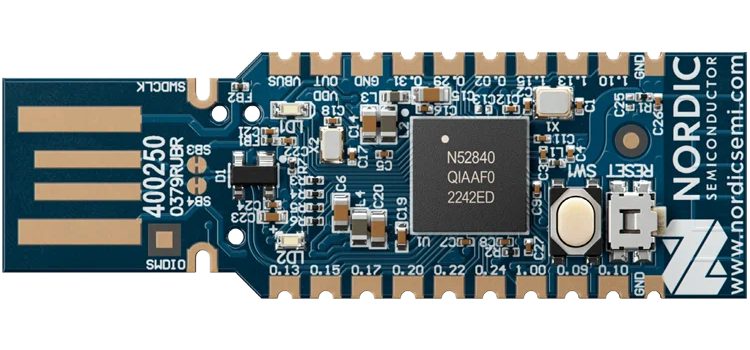
\includegraphics[width=0.4\textwidth]{img/nRF52840_Dongle.png}
\caption{nRF52840 Dongle. Źródło: \cite{nrf_dongle}}
\label{img:full_pcb}
\end{figure}

Na potrzeby sterownika do silników użyte zostało 12 pinów GPIO, 3 zostały przeprowadzone na zewnętrzne piny. Wyprowadzenia pinów układu nRF52840 Dongle:
\begin{itemize}
    \item 0.13 - PWM kanału B, połączone z układem Toshiby, odpowiada za kontrolę prędkości silnika B.
    \item 0.15 - PWM kanału A, jak wyżej.
    \item 0.17 - LO1, kod błędu zwracany przez układ Toshiby
    \item 0.20 - LO2, kod błędu zwracany przez układ Toshiby
    \item 0.22 - IN1 kanału A, pierwszy pin sterujący, odpowiadający za ustawienie kierunku ruchu silnika
    \item 0.24 - IN2 kanału A, drugi pin sterujący, jak wyżej.
    \item 1.00 - IN1 kanału B, jak wyżej.
    \item 0.09 - IN2 kanału B, jak wyżej.
    \item 0.10 - Enkoder 2 kanału B - pin odpowiadający za sprzężenie zwrotne od enkodera.
    \item 0.31 - P3, pin wolny przeprowadzony na zewnętrzny header.
    \item 0.29 - P1, jak wyżej.
    \item 0.02 - P2, jak wyżej.
    \item 1.15 - Enkoder 1 kanału A - pin odpowiadający za sprzężenie zwrotne od enkodera.
    \item 1.13 - Enkoder 2 kanału A - jak wyżej.
    \item 1.10 - Enkoder 1 kanału B - jak wyżej.
\end{itemize} \cite{nrf_mc_hw}

Znajomość wyżej opisywanych wyprowadzeń będzie przydatna w rozdziale \ref{cha:Software}, przy opracowywaniu oprogramowania odpowiedzialnego za kontrolę silnika.

\subsection{Toshiba TB67H420FTG Motor Controller}

TB67H420FTG to chip sterownika silników szczotkowych prądu stałego. Wewnętrzny mostek H można skonfigurować jako podwójny mostek dla jednego silnika, lub dwa pojedyncze mostki sterujące niezależnie dwoma osobnymi silnikami. Na potrzeby tego projektu opcja ta jest permanentnie ustawiona na dwa niezależne silniki za pomocą fizycznego przycisku na płytce, który zwiera odpowiedni pin chipu do masy. \cite{Toshiba_docs}

Jednakże najważniejsze piny z punktu widzenia tej pracy to piny mostka H, czyli IN1, IN2 oraz PWM, odpowiednio A i B w zależności od kanału. Opisują one zachowanie silnika w zależności od wejścia, jakie podamy na sterownik Toshiby. Zachowanie silnika w zależności od wartości tych 3 pinów przedstawia tabela \ref{table:Toshiba_pins}. W tabeli tej L oznacza stan niski pinu, zwarcie z masą, natomiast H stan wysoki, zwarcie z VCC. Należy także dodać, że jest to uproszczona wersja tabeli znajdującej się w rozdziale 3 dokumentacji \cite{Toshiba_docs}.

\begin{table}[h!]
\centering
\begin{tabular}{c | c c | c }
 PWM & IN1 & IN2 & tryb pracy silnika \\
 \hline
L & L & L & Standby Mode \\
L & - & - & Short Brake \\
H & L & L & Stop \\
H & H & L & Forward Rotation \\
H & L & H & Reverse Rotation \\
H & H & H & Short Brake \\
\end{tabular}
\caption{Uproszczona tabela trybów pracy sterownika TB67H420FTG. Źródło: \cite{Toshiba_docs}}
\label{table:Toshiba_pins}
\end{table}

Z punktu widzenia pisania późniejszego oprogramowania, można założyć, że Standby zachowuje się identycznie jak Stop. Tryby te powodują, że na silnik nie jest podawany prąd. Short Brake natomiast powoduje nagłe hamowanie oraz blokadę silnika. W tym trybie, prąd jest cały czas podawany na wyjście, co powoduje utrzymywanie silnika w miejscu. Najciekawsze natomiast są tryby Rotation, w których, jak sama nazwa wskazuje, silnik obraca się w zadanym kierunku, z prędkością proporcjonalną do wartości wypełnienia PWM.
    \chapter{Oprogramowanie Sterujące}
\label{cha:Software}
\section{Firmware - Oprogramowanie mikrokontrolera}
Firmware można podzielić na dwie części. Oprogramowanie open-source płytki sterownika do silników szczotkowych oraz właściwy skaner. Wspomniane oprogramowanie płytki sterownika wpiera już kontrolę prędkości obracania się pojedynczego silnika, oraz włączanie i wyłączanie silnika. Dodatkowo wspiera komunikację za pomocą komend powłoki (shell commands) transmitowanych po USB oraz Bluetooth LE. Na potrzeby tego projektu należy je rozwinąć o dodatkowy tryb kontroli - kontrola pozycji. Posiadając kontroler do silników szczotkowych zdolny do osiągnięcia zadanej pozycji, będzie możliwe napisanie wyższej warstwy abstrakcji - skanera, przyjmującego kolejne pozycje zgodnie ze zdefiniowaną macierzą punktów. Dodatkową zaletą podziału oprogramowania mikrokontrolera na dwie warstwy jest rozwój uniwersalnego sterownika do silników o kontrolę pozycji, który będzie można wykorzystać w wielu kolejnych projektach. Architektura ta przedstawiona jest na schemacie \ref{img:general_class_diag}.

\begin{figure}[h!] 
\centering 
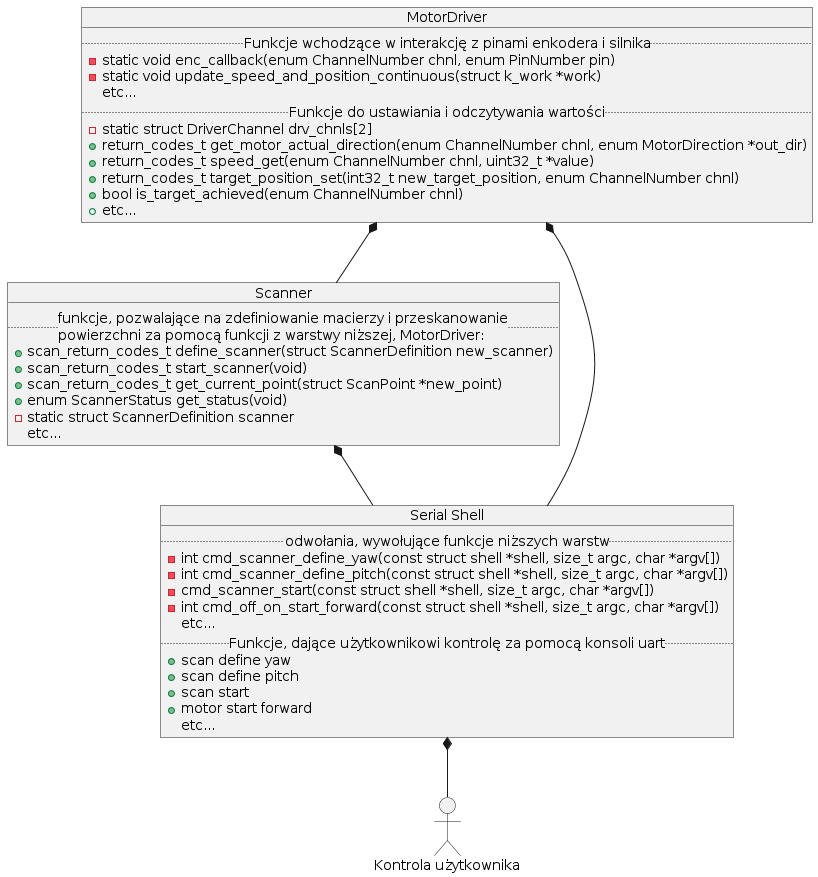
\includegraphics[width=0.9\textwidth]{img/ClassDiagGenUML.png}
\caption{Uogólniony schemat architektury oprogramowania}
\label{img:general_class_diag}
\end{figure}

Całość oprogramowania na mikrokontroler jest napisana w języku C, używając bibliotek HAL (Hardware Abstraction Layer) środowiska RTOS (Real Time Operataing System) Zephyr. Jest to zestaw open-sourcowych bibliotek, wspieranych między innymi przez firmę Nordic Semiconductors, która jest producentem procesora nRF52840. Głównymi zaletami Zephyra jest mały rozmiar budowanego kodu, wsparcie dla procesorów wielu producentów oraz licencja Apache 2.0. W architekturze Zephyra wsparcie różnych procesorów jest rozwiązane za pomocą Devicetree. Jest to oddzielny opis architektury wewnętrznej mikrokontrolera, jak piny, rejestry czy peryferia, ale też dodatkowych komponentów znajdujących się na płytce. Pozwala to na łatwe przenoszenie kodu między różnymi procesorami. \cite{Zephyr_docs}

Wspomniana na diagramie \ref{img:general_class_diag} architektura mocno opiera się o API programistyczne (\textbf{Application Programming Interface}; Interfejs Programowania Aplikacji). Jest to sposób, w jaki dwa programy albo komponenty oprogramowania wchodzą ze sobą w interakcję. \cite{api} Czyli upraszczając, w przypadku tego projektu jest to pewien zestaw publicznych funkcji i zmiennych, które w zaprojektowanej przez programistę bibliotece stanowią interfejs, za pomocą którego można z tą biblioteką wchodzić w interakcję. Wspomniane są także warstwy abstrakcji. Jako warstwę abstrakcji można uznać pewien zamknięty fragment kodu implementujący konkretną funkcjonalność, pozwalający na proste ponowne użycie tego fragmentu w kolejnym projekcie oraz zamykający skomplikowany kod za prostym interfejsem, np. poprzez zastosowanie pewnego API. \cite{abstraction_layer} Poprawne zaimplementowanie kodu, który stosuje zrozumiałe API oraz utrzymuje poprawny podział na warstwy abstrakcji, to pierwszy krok do zachowania zasad z grupy SOLID. Jest to mnemoniczny akronim pod którym kryje się 5 zasad tworzenia oprogramowania które jest skalowalne, zrozumiałe oraz łatwe w utrzymaniu. \cite{solid}

\subsection{Skalowalne rozwiązanie wielokanałowe}
\label{cha:second_channel}
Na potrzeby kontroli pozycji dookoła dwóch osi, należało zrefaktoryzować obecną kontrolę prędkości oraz zaimplementować nową kontrolę pozycji w sposób skalowalny. W celu osiągnięcia tego założenia, powstała struktura, opisująca pojedynczy kanał kontrolera. Jej interfejs przedstawiony jest na \ref{img:driver_channel_diag}.

\begin{figure}[h!] 
\centering 
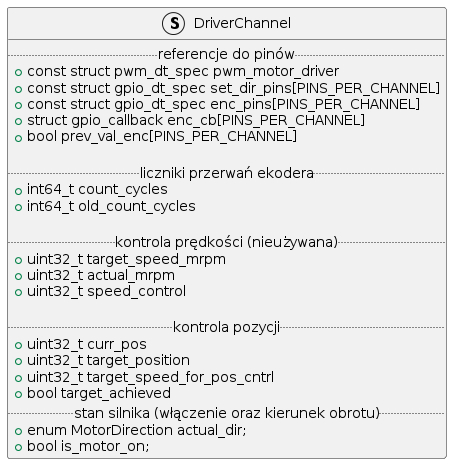
\includegraphics[width=0.5\textwidth]{img/DriverChannelUML.png}
\caption{Interfejs struktury opisującej kanał sterownika.}
\label{img:driver_channel_diag}
\end{figure}

Następnie została utworzona skalowalna tablica kanałów \texttt{drv\_chnls} typu \texttt{static struct DriverChannel}. W przypadku tego projektu ma ona zaledwie 2 elementy, ale może być skalowana dowolnie, w zależnie od możliwości sprzętowych. Opisywana lista struktur zaimplementowana jest wewnątrz pliku driver.c (który zawiera implementację sterownika) i jedynie funkcje z tego pliku mają do niej dostęp.

Każda funkcja ze wspominanego pliku przyjmuje numer kanału typu \texttt{enum ChannelNumber}. Wewnątrz poszczególnych funkcji numer kanału stanowi odniesienie do odpowiedniego elementu wcześniej opisywanej tablicy. Jest to dobry przykład architektury open-closed (litera O ze skrótu SOLID), gdzie programista daje użytkownikowi jedynie zestaw funkcji, tutaj zdefiniowanych w pliku driver.h, za pomocą których użytkownik (programista używający API) odnosi się do wewnętrznej, zamkniętej implementacji, która może ulec zmianie, bez wpływania na interfejs użytkownika.

\subsection{Kontrola pozycji silnika szczotkowego}
\label{cha:pos_control}
\subsubsection{Przerwanie od pinów enkodera}
Podstawą precyzyjnego wyznaczania pozycji silnika szczotkowego jest poprawnie działające przerwanie od enkodera. Enkoder pojedynczego silnika składa się z dwóch pinów, podczas normalnej pracy - obracania się ze stałą prędkością w jednym kierunku - na piny te podawana jest fala prostokątna, przesunięta w fazie o $\frac{1}{4}$ okresu. Przesunięcie to pozwala na wyznaczenie kierunku ruchu silnika. Dla pinu 1, jeżeli wartości pinów są różne, to silnik kręci się do przodu, jeżeli takie same, to w przeciwnym kierunku. W przerwaniu od pinu 2 jest na odwrót - dla wartości takich samych obrót następuje do przodu. Dalej w zależności od kierunku, następuje inkrementacja bądź dekrementacja licznika. \cite{rotary_encoder_tutorial} Funkcja, odpowiedzialna za zliczanie przerwań, przedstawiona jest na schemacie \ref{img:encoder_callback}. Jest to przepływ logiki zaprezentowany jedynie dla jednego kanału. Cały ten proces wykonywany jest osobno dla obu kanałów, a dodatkowo na \ref{img:driver_channel_diag} widać, że faktycznie, \texttt{count\_cycles} jest zdefiniowany osobno, dla obu kanałów.

\begin{figure}[h!] 
\centering 
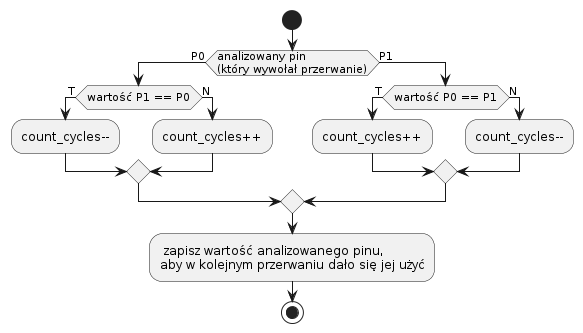
\includegraphics[width=0.8\textwidth]{img/PinInterruptUML.png}
\caption{Przepływ logiki przerwania od pinu enkodera na pojedynczym kanale.}
\label{img:encoder_callback}
\end{figure}

\subsubsection{Przerwanie od zegara}
Przerwanie od enkodera może być wywoływane bardzo często - przy maksymalnej prędkości użytego silnika ponad 10 razy na milisekundę ($\frac{RPM \cdot CPR}{60 \cdot 1000} = \frac{67 \cdot 9600}{60 * 1000} = 10.72 $), a należy pamiętać że jest to najwolniejszy silnik z tej linii produktu. Biorąc pod uwagę, że efektem tej pracy ma być uniwersalny sterownik do silników, trzeba uwzględnić także szybsze jednostki. Z tego powodu nie można umieszczać w tym przerwaniu zbyt zaawansowanego kodu, jedynie podstawowe obliczenia, jak inkrementacja odpowiedniej zmiennej. Właściwe obliczenia pozycji, a także prędkości, której kontrolę także trzeba utrzymać aby zachować wsteczną kompatybilność, są realizowane w osobnym przerwaniu, od zegara, które jest wywoływane co $20ms$. Czas tego przerwania jest zmienną czasu kompilacji i może być swobodnie dostosowywany w pliku \texttt{prj.conf}, w zależności od potrzeb projektowych. Oczywiście im ten czas będzie mniejszy, tym kontrola powinna być precyzyjniejsza, ponieważ przerwanie obliczające obecną pozycję, prędkość i kierunek ruchu będzie wywoływane częściej. Ale też należy pamiętać, że im częściej przerwanie to będzie wywoływane, tym większe ryzyko, że kolejne przerwanie rozpocznie się, zanim poprzednie się zakończy, co przy obecnej implementacji spowoduje, że kolejka zadań (task work queue) zapcha się i procesor zawiesi się. Jest to problem, który da się jedynie rozwiązać zastosowaniem mocniejszego (na przykład wielowątkowego) procesora lub zmniejszeniem częstotliwości przerwań.

Przerwanie od zegara jest najważniejszą funkcją całego sterownika. To w niej dzieją się całe obliczenia. Na potrzeby kontroli pozycji powstały dwa duże, istotne, fragmenty tej funkcji. Pierwszym z nich jest odczytywanie obecnej pozycji, przedstawione na schemacie \ref{img:pos_calc_UML}. Jest to wykonywane zawsze, w każdym cyklu przerwania, dla każdego kanału. Drugim fragmentem jest sama kontrola pozycji, przedstawiona na schemacie \ref{img:pos_settin_UML}. Kod ten jest zależny od wartości stałych kompilacyjnych. Zostanie wywołany tylko przy ich odpowiednich wartościach, które na potrzeby tego projektu zostały ustawione w kombinacji - kontrola pozycji włączona, prędkości wyłączona. Rozróżnienie takie jest wymagane aby zachować wsteczną kompatybilność z poprzednimi projektami.

\subsubsection{Obliczanie pozycji}
\label{cha:calc_pos}

\begin{figure}[h!] 
\centering 
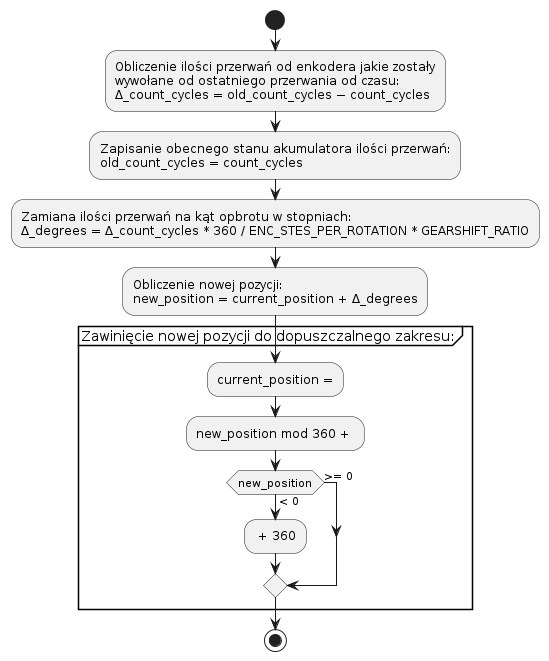
\includegraphics[width=0.8\textwidth]{img/CalcNewPos.png}
\caption{Diagram obliczania obecnej pozycji dla jednego kanału.}
\label{img:pos_calc_UML}
\end{figure}

Obliczanie pozycji odbywa się w kilku krokach. Pierwszy krok to obliczenie przyrostu ilości przerwań enkodera od ostatniego wywołania przerwania od czasu. Znając obecną wartość akumulatora \texttt{count\_cycles}, oraz jego wartość która została zapisana podczas poprzedniego cyklu, można obliczyć różnicę $\Delta_{count\_cycles} = old\_count\_cycles - count\_cycles$. Następnie po tych obliczeniach obecna wartość \texttt{count\_cycles} jest zapisywana dla zmiennej \texttt{old\_count\_cycles}, na potrzeby kolejnego przerwania od czasu. Kolejny krok, to skalowanie, zamiana jednostek - przeliczenie $\Delta_{count\_cycles}$, na stopnie. Odbywa się to za pomocą wzoru \ref{eq:cycles_to_deg}. Wzór ten zawiera zmienne \texttt{ENC\_STEPS\_PER\_ROTATION} oraz \texttt{GEARSHIFT\_RATIO}, które są zmiennymi czasu kompilacji zdefiniowanymi w pliku Kconfig.motor, i ich wartości powinny odpowiadać wartościom odczytanym z dokumentacji użytych silników. Dla silnika Pololu 2828 wynoszą odpowiednio:
\vspace{-\topsep}
\begin{itemize}
    \item \texttt{ENC\_STEPS\_PER\_ROTATION = 64},
    \item \texttt{GEARSHIFT\_RATIO = 150},
\end{itemize}
\vspace{-\topsep}

\begin{equation}
\label{eq:cycles_to_deg}
    \Delta_{degrees} = \frac{\Delta_{count\_cycles} \cdot 360^{\circ}}
		  {ENC\_STEPS\_PER\_ROTATION \cdot GEARSHIFT\_RATIO}
\end{equation}

Kolejny krok jest bardzo prosty, polega na dodaniu obliczonej $\Delta_{degrees}$ do akumulatora \texttt{current\_position}, przechowującego ostatnią faktyczną pozycję silnika. Tutaj należy pamiętać, że w zależności od kierunku obrotu silnika wartość $\Delta_{degrees}$ może być ujemna. Może to spowodować, że \texttt{current\_position} przyjmie także wartość ujemną. Nie jest to pożądana sytuacja, jako że idea stojąca za wspomnianą zmienną jest inna - powinna ona przechowywać wartość z zakresu $0 - 360^{\circ}$. Dlatego też nie następuje od razu przypisanie nowej wartości do tej zmiennej. Obecna wartość zmiennej \texttt{current\_position} jest tymczasowo zamieniana z typu \texttt{unsigned int} na \texttt{int}, co pozwala na użycie jej ze znakiem. Następnie nowa wartość jest przenoszona do zakresu $0 - 360^{\circ}$ zgodnie ze wzorem \ref{eq:wrap_current_deg_pos}, aby na samym końcu nadpisać starą wartość zmiennej.

\begin{equation}
\label{eq:wrap_current_deg_pos}
    current\_position = ( new\_position \mod 360^{\circ} ) + 
    \begin{cases}
      360^{\circ} & \text{jeżeli } new\_position < 0\\
      0 & \text{w przeciwnym wypadku}\\
    \end{cases}
\end{equation}

Cały algorytm, opisywany w tym rozdziale, został zamknięty w trzech makrach, co pozwala na jego zapis w zaledwie jednej linijce kodu i bardzo szybki czas wykonania. W celu lepszej wizualizacji, został on także zaprezentowany w formie diagramu \ref{img:pos_calc_UML}. Rysunek ten przedstawia algorytm dla jednego kanału. Makra odpowiedzialne za wspomniane obliczenia przyjmują jako argument także numer kanału i odnoszą się do odpowiednich zmiennych, zdefiniowanych jako część danego kanału.



\subsubsection{Ruch do pozycji docelowej}
Ruch do pozycji docelowej jest bardziej skomplikowanym spośród dwóch algorytmów wykonywanych w ramach cyklicznego przerwania od czasu. W pierwszej kolejności należy obliczyć deltę, różnicę między punktem obecnym a punktem docelowym. Wartość oraz znak tej różnicy będą w pierwszej kolejności mówiły o kierunku, w którym powinien zacząć obracać się silnik. Jest to widoczne w pierwszej części schematu przedstawionego na rys. \ref{img:pos_settin_UML}. Widać, że wartość absolutna tej różnicy wpływa na to, od której strony wał dotrze do punktu docelowego. Jeżeli jest większa od $180^{\circ}$, to silnik dotrze do punktu "od tyłu", natomiast jeżeli jest mniejsza, to dotrze do punktu "od przodu". Natomiast znak wartości tej różnicy - część schematu sprawdzająca, czy zmienna \texttt{position\_delta} jest ujemna czy dodatnia - odpowiada za ustalenie po której stronie obecnej pozycji wału silnika znajduje się "przód"\ punktu, a po której "tył"\ punktu.

\begin{figure}[h!] 
\centering 
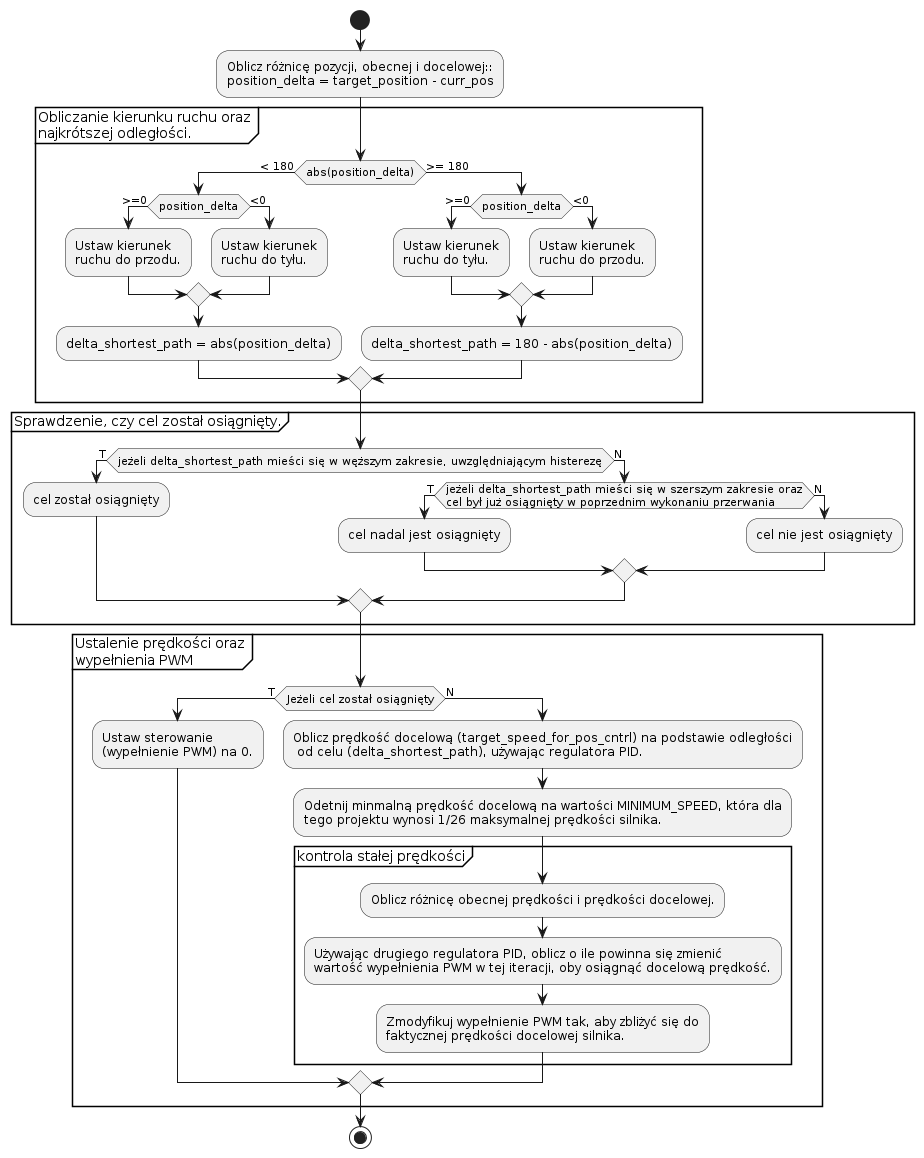
\includegraphics[width=\textwidth]{img/PosSettingUML.png}
\caption{Ruch do pozycji docelowej.}
\label{img:pos_settin_UML}
\end{figure}

Kolejnym fragmentem diagramu \ref{img:pos_settin_UML} jest sprawdzenie, czy wał silnika osiągnął zadaną pozycję docelową. Z powodu problemu, jaki pojawił się w czasie testów urządzenia, musi odbywać się to w dwóch krokach. Po osiągnięciu pozycji, napięcie na przekładni połączone z masą poruszanego obiektu powodowały, że wał silnika cofał się o kilka setnych stopnia. W zależności od jego dokładnej pozycji, mogło to spowodować opuszczenie dopuszczalnego zakresu. Dlatego też wymusiło to dodanie swego rodzaju histerezy. I to właśnie wspomniana histereza jest sprawdzana w pierwszej kolejności. Ogranicza ona dopuszczalny zakres kątów o pewien procent, co wymusza na sterowniku precyzyjniejszą kontrolę właśnie o ten procent. Natomiast, aby wyeliminować opisywany powyżej problem, główny dopuszczalny obszar jest nieco szerszy. Jeżeli w poprzednim wykonaniu przerwania osiągnięty już został obszar węższy, uwzględniający histerezę, to w kolejnym wykonaniu dopuszczalny obszar jest odrobinę większy. Eliminuje to ryzyko, że mikro ruchy na granicy obszaru wymuszą ponowny ruch wibrometru i jego ponowną próbę osiągnięcia wymaganego zakresu. Obszary te są zdefiniowane jako zmienne kompilacyjne w pliku prj.conf i wynoszą:
\vspace{-\topsep}
\begin{itemize}
    \item \texttt{POS\_CONTROL\_PRECISION\_MODIFIER = 480}, co daje obszar $\pm 0.75^{\circ}$
    \item \texttt{POS\_CONTROL\_HISTERESIS\_PERCENTAGE = 40\%}, co daje obszar $\pm 0.3^{\circ}$
\end{itemize}

Ostatnim, najbardziej istotnym, fragmentem ustalania pozycji jest sam regulator PID (\textbf{Proportional–integral–derivative controller}, regulator proporcjonalno-całkująco-różniczkujący), a raczej tandem dwóch regulatorów PID. W pierwszej kolejności na podstawie wcześniej obliczonej, najkrótszej odległości od celu ustalona zostaje prędkość, z jaką powinien kręcić się silnik. Prędkość ta jest proporcjonalna do odległości, zgodnie z zasadą działania człona P regulatora. Jest ona także odcinana na minimalnej ustalonej wartości prędkości, aby wyeliminować problemy pojawiające się przy próbie wymuszenia bardzo małych prędkości silnika szczotkowego. W tym miejscy należy zwrócić uwagę, że wyjściem tego regulatora jest prędkość. Sterowaniem całego układu jest natomiast wypełnienie PWM, od którego prędkość jest zależna. Jednakże, zwłaszcza przy zastosowaniu znacznych obciążeń, ta zależność nie będzie liniowa. Dlatego też został zaimplementowany drugi regulator PID, który na wejście otrzymuje wcześniej obliczoną prędkość docelową oraz faktyczną obecną prędkość silnika. Natomiast jego wyjściem jest przyrost wartości wypełnienia,  wymagany aby otrzymać faktyczną docelową prędkość silnika. Tak zmodyfikowana wartość wypełnienia PWM jest podawana na układ sterownika Toshiba.

Wspomniany wyżej regulator PID został zaimplementowany zgodnie z uproszczonym wzorem \ref{eq:pid_equation}, gdzie $\Delta_{akumulator}$ oznacza sumę wszystkich poprzednich wartości $\Delta$, natomiast $\Delta_{poprzednia\_wartość}$ oznacza wartość $\Delta$ z poprzedniego wykonania przerwania. $\Delta$ natomiast to tak zwany błąd, czyli różnica między wartością (czy prędkości, czy pozycji) obecną, a docelową. Parametry $Kp$, $Ki$ oraz $Kd$ to nastawy regulatora, dobierane indywidualnie na potrzeby projektu.

\begin{equation} \label{eq:pid_equation}
    sterowanie = Kp \cdot \Delta + Ki \cdot \Delta_{akumulator} + Kd \cdot \Delta_{poprzednia\_wartosc}
\end{equation}

Nastawy obu regulatorów PID zostały dobrane empirycznie, tak aby sprawdzały się przy małych prędkościach obrotu, jeden komplet dla obu kanałów. Podczas dostrajania został użyty jedynie człon P, a wartości $Ki$ oraz $Kd$ zostały ustawione na $0$. Użycie tych członów okazało się nie być potrzebne do poprawnego ruchu wibrometru. Ostatecznie wartości $Kp$ dla dwóch kolejnych regulatorów zostały kolejno ustawione na:
\vspace{-\topsep}
\begin{itemize}
    \item $Kp_{kontroli\_pozycji} = 2\frac{1}{2}$
    \item $Kp_{kontroli\_predkości} = \frac{1}{2}$
\end{itemize}

W tym miejscu, tak samo jak w przypadku rozdziału \ref{cha:calc_pos}, należy pamiętać, że algorytm przedstawiony na schemacie \ref{img:pos_settin_UML} ilustruje jedynie przepływ logiki dla jednego kanału. W ramach opisywanego przerwania od czasu, jest on wykonywany dwa razy, osobno dla obu kanałów, a opisywane zmienne stanowią część listy struktur opisywanej w rozdziale \ref{cha:second_channel} oraz są przedstawione na diagramie \ref{img:driver_channel_diag}.

\subsection{Algorytm skanujący}
\label{cha:scan_alg}
Algorytm korzysta z API, będącego interfejsem niższej warstwy oprogramowania, opisywanej w rozdziale \ref{cha:pos_control}. API udostępnia interfejsy pozwalające kontrolować pozycję silników na poszczególnych kanałach i jest zaprojektowane w taki sposób, aby algorytmy stojące za kontrolą pozycji nie miały wpływu na pracę programisty tworzącego warstwę skanera.

Cały proces skanowania zaczyna się od zdefiniowania oraz przygotowania skanera, a odpowiedzialna jest za to funkcja \texttt{define\_scanner}. Funkcja ta przygotowuje kontroler poprzez wyłączenie silników (tylko jeżeli użytkownik zostawił je włączone po poprzedniej operacji) oraz ustawienie odpowiedniego trybu pracy - kontroli pozycji. Następnie ustawia wewnętrzną instancję skanera, znajdującego się pod zmienną \texttt{struct ScannerDefinition scanner} na definicję skanera przekazaną jako argument do funkcji. Definicja ta jest typu \texttt{struct ScannerDefinition}, który opisuje wszystkie parametry definiowanego skanera. Struktura ta jest przedstawiona na schemacie \ref{img:scanner_def_uml}.

\begin{figure}[h!] 
\centering 
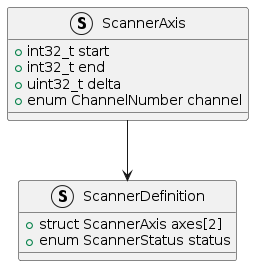
\includegraphics[width=0.4\textwidth]{img/ScannerDefUML.png}
\caption{Struktura opisująca parametry skanera.}
\label{img:scanner_def_uml}
\end{figure}

Na schemacie \ref{img:scanner_def_uml} widać także wzmiankę o statusie skanera. Także znaczna większość funkcji, włącznie z definiowaniem skanera, zawiera sprawdzenia statusów. Koncept maszyny stanów statusów skanera jest dokładnie wyjaśniony w rozdziale \ref{cha:state_machine}.


Kolejnym krokiem algorytmu jest startowanie skanera. Start, poza standardowymi sprawdzeniami statusu, ustawia obecny cel (zmienna \texttt{target}) i przekazuje ten cel warstwę niżej, poprzez API sterownika do silników, za pomocą funkcji \texttt{target\_position\_set}. Odbywa się też wtedy start zegara \texttt{wait\_for\_point\_timer}, którego przerwanie ma za zadanie sprawdzać, czy punkt zadany został już osiągnięty. Logika tejże funkcji przedstawiona jest na \ref{img:wait_for_point_handler}.

\begin{figure}[h!] 
\centering 
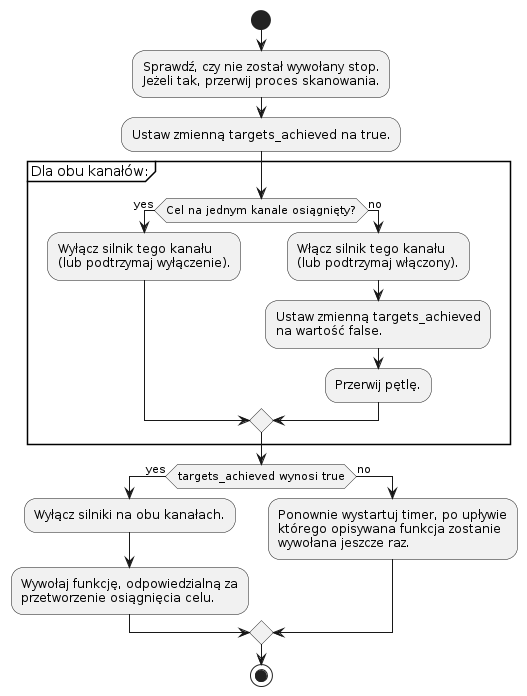
\includegraphics[width=0.7\textwidth]{img/WaitForPointUML.png}
\caption{Przepływ logiki funkcji \texttt{wait\_for\_point\_handler()}.}
\label{img:wait_for_point_handler}
\end{figure}

Diagram \ref{img:wait_for_point_handler} pokazuje logikę, którą można opisać jako utrzymywanie jednego kanału włączonego, dopóki cel nie jest osiągnięty, a następnie załączenie drugiego kanału. Natomiast pod koniec wspomniana jest funkcja, która przetwarza osiągnięcie celu przez oba kanały (na obu osiach urządzenia). Funkcja ta, jest głównym miejscem całego algorytmu, gdzie podejmowane są decyzje oraz wykonywane wszystkie istotne obliczenia. Przepływ logiki tejże funkcji przedstawiony jest na diagramie \ref{img:point_achieved_handler}.

\begin{figure}[h!] 
\centering 
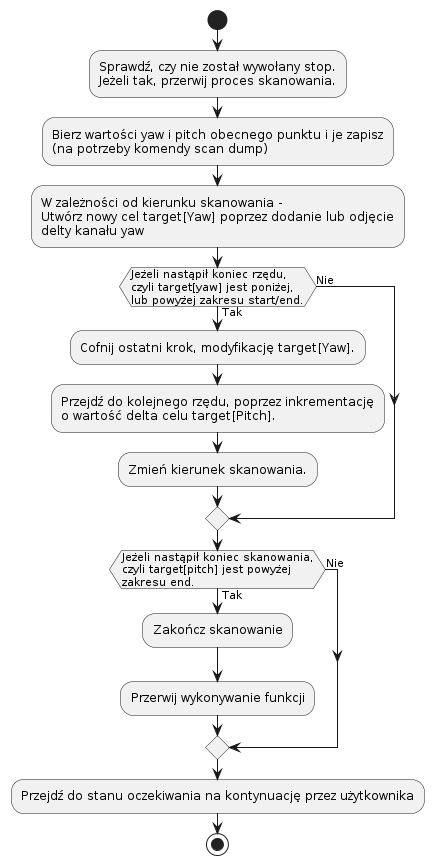
\includegraphics[width=0.6\textwidth]{img/PointAchievedUML.png}
\caption{Przepływ logiki funkcji \texttt{point\_achieved\_handler()}.}
\label{img:point_achieved_handler}
\end{figure}

Patrząc na diagram \ref{img:point_achieved_handler} można wywnioskować, że funkcja \texttt{point\_achieved\_handler()} odpowiedzialna jest za podjęcie decyzji, jakie mają być wartości kolejnego punktu, do którego będzie zmierzać urządzenie. Schemat jej działania można uprościć do opisu: Wpierw następuje przeskanowanie pierwszego rzędu, zwiększając cel na osi yaw z każdym wywołaniem tej funkcji. Następnie, jeżeli kolejny punkt miałby przekroczyć wartość zdefiniowaną jako \texttt{yaw\_end} funkcja ta zmienia rząd, oraz kierunek ruchu silnika umieszczonego w osi yaw (pionowej, z). Jeżeli zwiększenie rzędu miałoby spowodować wartość na osi pitch większą niż \texttt{pitch\_end} - następuje zakończ skanowanie.

Funkcja, jak wskazano na diagramie \ref{img:point_achieved_handler} kończy się oczekiwaniem na reakcję użytkownika. Reakcja następuje po wywołaniu funkcji \texttt{move\_to\_next\_point()}. Działa ona bardzo podobnie do startu, z pominięciem ustawiania nowego celu, cel został już ustawiony. Podaje ona jedynie te cele do funkcji \texttt{target\_position\_set} i startuje zegar \texttt{wait\_for\_point\_timer}. W tym momencie następuje powrót do odwołania od tego zegara opisanego w \ref{img:wait_for_point_handler}.

\subsection{Maszyna stanów urządzenia}
\label{cha:state_machine}
\begin{figure}[h!] 
\centering 
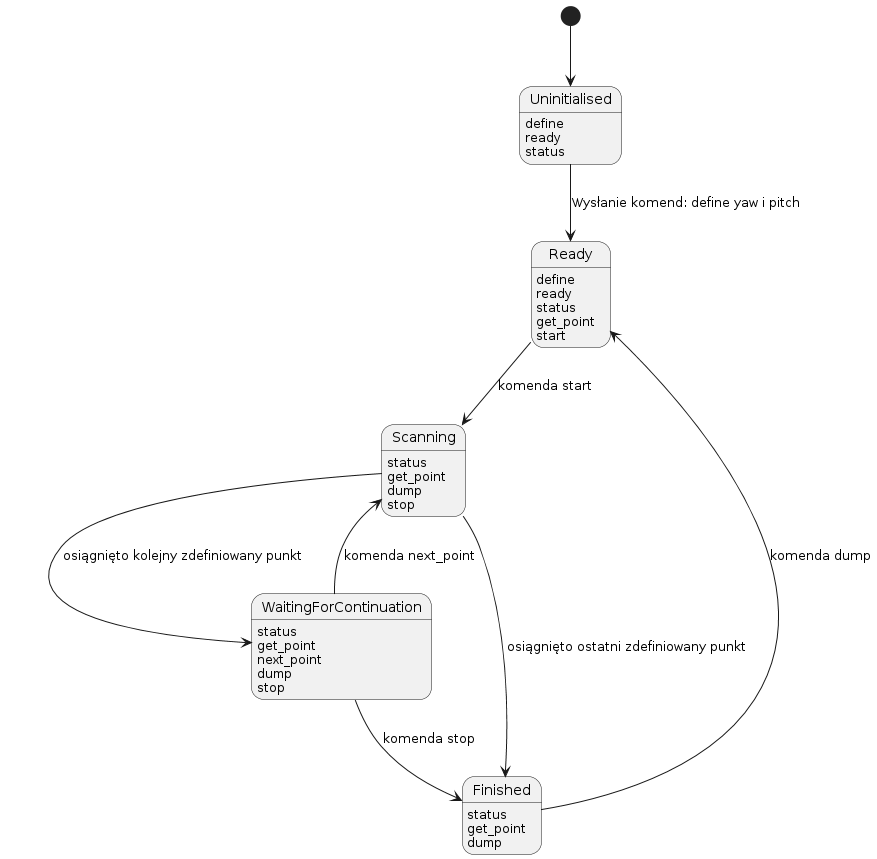
\includegraphics[width=\textwidth]{img/StatesUML.png}
\caption{Maszyna stanów urządzenia.}
\label{img:states_uml}
\end{figure}
Aby zabezpieczyć urządzenie przed wykonywaniem niedozwolonych operacji, oraz potencjalnym uszkodzeniem, powstała maszyna stanów, a każda funkcja jest ograniczona do określonych stanów, w których jej wywołanie jest dopuszczalne. Maszyna stanów jest przedstawiona na diagramie \ref{img:states_uml}. Są na nim rozpisane wszystkie stany, wraz z dopuszczalnymi funkcjami. Stanowi on także dobrą prezentację logiki przedstawionej w rozdziale \ref{cha:scan_alg}. Działanie poszczególnych funkcji jest wyjaśnione w rozdziale \ref{cha:commands}.

\subsection{Serial Shell}
\label{cha:usb}
Procesor nRF52840 zawiera peryferia obsługujące wiele różnych protokołów komunikacyjnych. Na potrzeby tego projektu zdecydowano się na komunikację szeregową za pomocą popularnego protokołu USB 2.0 i szeregowego interfejsu powłoki (\textbf{serial shell}), zaimplementowanego na wierzchu USB. Peryferium to jest obsługiwane z poziomu procesora przez zestaw sterowników Communication Device Class: Abstract Control Model (\textbf{CDC ACM}), które stanowią integralną część bibliotek Zephyra. Powoduje to, że po podłączeniu po USB do komputera PC, urządzenie zgłasza się jako wirtualny port COM. \cite{nrf_52840_docs}

Jest to o tyle ciekawe rozwiązanie, że zwykle stosuje się peryferium obsługujące komunikację po protokole UART (\textbf{Universal Asynchronus Reciever/Transmitter}) i dodatkowy zewnętrzny konwerter UART-USB, i to ten kontroler zgłasza się jako wirtualny port COM. Wymusza to na użytkowniku zdefiniowanie parametrów komunikacji UART między konwerterem a procesorem. Tutaj te parametry są niepotrzebne, ponieważ nie ma tego dodatkowego połączenia szeregowego. W rozwiązaniu tym wirtualne COM-porty, które normalnie służą do symulacji szeregowych interfejsów sprzętowych,  używane są do podpięcia się do urządzenia bezpośrednio po protokole USB. \cite{nrf_52840_docs}

\subsubsection{Łączenie z urządzeniem}
\label{cha:COM_connect}
Tak jak już wspomniano, po podłączeniu kablem USB do komputera, urządzenie zgłosi się jako wirtualny port COM.

\begin{minipage}{\textwidth}
Listę podpiętych COM portów można uzyskać w różny sposób w zależności od systemu operacyjnego:
\begin{itemize}
    \item Windows: \cite{identify_com_ports_win}
    \begin{enumerate}
        \item Otworzyć Menadżer Urządzeń.
        \item Zlokalizować sekcję Porty (COM \& LPT).
        \item Rozwinąć ją.
    \end{enumerate}
    \item Linux - komenda \texttt{ls /sys/class/tty/tty*} (lub podobna, w zależności od dystrybucji.) \cite{identify_com_ports_linux}
    \item MacOS - komenda \texttt{ls /dev/tty.*} \cite{identify_com_ports_macos}
\end{itemize}
\end{minipage}

\begin{minipage}{\textwidth}
\noindent Uwaga!
\vspace{-\topsep}
\begin{itemize}
    \item Na każdym komputerze urządzenie może zgłaszać się pod innym numerem.
    \item Jeżeli widnieje tam więcej niż jeden COM port, najlepszym rozwiązaniem jest wypiąć urządzenie, sprawdzić co znikło oraz wpiąć je ponownie.
\end{itemize}
\end{minipage}

\vspace{\topsep}

Nazwa, pod jaką zgłasza się urządzenie, jest potrzebna aby otworzyć z nim połączenie. Można to zrobić za pomocą dowolnego terminala wspierającego połączenie szeregowe. Dobrym przykładem takiego terminala jest program PuTTY. Po otworzeniu go, należy przejść do zakładki Serial (Połączenie szeregowe), wpisać numer portu, oraz otworzyć połączenie. Zwykle istnieją też inne parametry które można ustawić, jak na przykład prędkość transmisji (\textbf{baudrate}). Lecz tak jak wspomniano wyżej, ich definiowanie, dzięki rozwiązaniom sprzętowym zaimplementowanym w procesorze, nie jest potrzebne.

\subsubsection{Komendy udostępniane przez urządzenie}
\label{cha:commands}
Zephyr RTOS umożliwia komunikację z urządzeniem za pomocą tzw. komend powłoki (\textbf{shell commands}). Udostępnia on dodatkową warstwę abstrakcji, która interpretuje po stronie urządzenia znaki przychodzące jako tekst i wywołuje funkcje, odpowiednio przypisane do kolejnych komend. Z perspektywy użytkownika końcowego, daje to możliwość komunikacji z urządzeniem za pomocą zwyczajnego tekstu - komend przypominających te z konsoli systemów typu unix. Wartości kolejnych bajtów, przesyłanych po USB, stają się nieistotne dla końcowego użytkownika.

Najważniejsza komenda którą trzeba znać to komenda \texttt{help}. Po wysłaniu tego łańcucha znaków do urządzenia, użytkownik dostanie odpowiedź zawierającą informacje o wszystkich wspieranych komendach, których lista znajduje się poniżej:

\begin{itemize}
    \item komendy skanera:
    \begin{itemize}
        \item \texttt{scan define yaw} - Definiowanie osi yaw (obrotu dookoła z) skanera.
        
        Argumenty: <kanał HW> <start deg> <stop deg> <delta deg>

        Które po kolei oznaczają: kanał na który fizycznie jest wpięty silnik, wartość w decy-stopniach na której silnik ma wystartować, wartość końcowa oraz krok z jakim ma się przemieszczać.

        \item \texttt{scan define pitch} - Definiowanie osi pitch (obrotu dookoła y) skanera.

        Argumenty oraz ich znaczenie jak wyżej. Wspólnie, te dwie komendy definiują macierz punktów które wibrometr przeskanuje.

        \item \texttt{scan ready} - Sprawdzenie gotowości skanera, czy obie osie są poprawnie zdefiniowane, oraz przygotowanie silników.

        \item \texttt{scan start} - Wystartowanie skanera, przemieszczenie na zdefiniowany punkt początkowy (yaw start; pitch start)

        \item \texttt{scan status} - Sprawdzenie, w jakim statusie znajduje się skaner. Dokładny opis oraz znaczenie statusów znajduje się w rozdziale \ref{cha:state_machine}.

        \item \texttt{scan get\_point} - Zebranie punktu, w którym znajduje się obecnie urządzenie.

        \item \texttt{scan next\_point} - Wywołanie ruchu do kolejnego zdefiniowanego punktu. (Tylko jeżeli skaner osiągnął punkt poprzedni.)

        \item \texttt{scan dump} - Zrzut wszystkich punktów, w których zatrzymał się skaner od początku pomiaru, bądź ostatniego wywołania komendy. Dodatkowo, komenda ta czyści status "finished"\ i przenosi urządzenie w status "ready"

        \item \texttt{scan stop} - Przedwczesne przerwanie pracy skanera.        
    \end{itemize}
    \item komendy niezależnej kontroli pozycji:
    \begin{itemize}
        \item \texttt{channel} - Komenda pusta, zbiera wartość obecnie aktywnego kanału. Podanie argumentu, 0 lub 1, spowoduje aktywowanie odpowiedniego kanału. Wszystkie poniższe komendy tyczą się tylko jednego, aktywnego kanału.

        \item \texttt{pos} - Komenda pusta, zbierze pozycję, na której znajduje się obecnie silnik. Dodanie argumentu spowoduje ustawienie nowej pozycji docelowej.

        \item \texttt{pos zero} - Komenda ustawiająca obecną pozycję silnika jako pozycja "zero".

        \item \texttt{motor} - Komenda pozwalająca odczytać, czy silnik jest włączony czy wyłączony.

        \item \texttt{motor start} - Komenda uruchamiająca silnik.

        \item \texttt{motor stop} - Komenda wyłączająca silnik.

        \item \texttt{speed} - Komenda pozwalająca odczytać obecną prędkość silnika w mili RPM-ach.

        \item \texttt{actual\_direction} - Komenda pozwalająca odczytać kierunek kręcenia się silnika.
    \end{itemize}
\end{itemize}

Uwaga! Istnieją też komendy \texttt{drv\_version} oraz \texttt{scan version}. Dają one informacje o wersjach oprogramowania warstwy sterownika oraz skanera. W ramach pracy opracowane zostały wersje:
\vspace{-\topsep}
\begin{itemize}
    \item skaner = 1.0
    \item sterownik = 2.5
\end{itemize}
\vspace{-\topsep}
Inne wersje mogą implementować inne funkcje, lub istniejące funkcje mogą działać nieco inaczej.

Komunikacja za pomocą komend konsoli jest bardzo prosta koncepcyjnie, jednakże może być uciążliwa dla końcowego użytkownika. Dlatego też w ramach pracy opracowano programy, które ułatwiają tą komunikację. Są one przedstawione w rozdziale \ref{cha:host_apps}.

\subsection{Skaner automatyczny}
\label{cha:auto_scanner}
W ramach pracy zostały także podjęte kroki, w celu zamknięcia całego procesu skanowania wewnątrz procesora, tak aby można było dokonać całego pomiaru bez potrzeby wchodzenia w interakcję z urządzeniem podczas skanowania.

Przede wszystkim powstała zmienna kompilacyjna, definiująca czy skan ma być automatyczny czy semi-manualny. Pod wartością, odpowiadającą skanowi automatycznemu, kryje się kilka zmian względem algorytmów opisanych w rozdziałach \ref{cha:scan_alg} - \ref{cha:usb}.

Zamiast stanu WaitingForContinuation, urządzenie wymaga zdefiniowania także czasu, jaki zajmuje mu ustabilizowanie się po osiągnięciu pozycji. Czas ten powinien zostać znaleziony empirycznie i wiąże się z elementami takimi jak wymóg uspokojenia się drgającej konstrukcji po zatrzymaniu. Kolejną zmianą jest uruchomienie przetwornika analog cyfra (\textbf{ADC}, \textbf{Analog-Digital Converter}) wbudowanego w mikrokontroler. Bufor, przetrzymujący odwiedzone przez wibrometr punkty, w trybie automatycznego skanowania, przetrzymuje także wartości zmierzone za pomocą układu ADC.

Na tym zakres wykonanych prac się zakończył, ponieważ okazało się, że górny limit wejścia napięciowego przetwornika ADC znajdującego się na pokładzie miktokontrolera jest równy napięciu zasilania, które maksymalnie może wynosić $5.5V$, a wibrometr pracuje w zakresie do $10V$.

Kolejne kroki, jakie powinny zostać podjęte aby w pełni zautomatyzować pomiar za pomocą samego układu wbudowanego, to podpięcie po I\textsuperscript{2}C lub SPI zewnętrznego ADC spełniającego kryteria wyjścia napięciowego wibrometru. Kolejno, należałoby poprawić bufor, w taki sposób aby wspierał pomiar składający się z wielu próbek w każdym punkcie, oraz zaimplementować algorytm przetwarzania sygnałów po stronie mikrokontrolera.

\section{Hostapp - Oprogramowanie sterujące}
\label{cha:host_apps}
Jak już wspomniano, urządzeniem można sterować tylko i wyłącznie przy pomocy konsoli serialowej. Jednakże większość współczesnych języków programowania wspiera wysyłanie komend za pomocą protokołu szeregowego, co daje możliwości stworzenia bardziej przyjaznych interfejsów użytkownika.

\subsection{Matlab API}
\label{cha:matlab_api}
Najprostszym sposobem zebrania danych z samego wibrometru jest użycie programu Matlab. Dlatego też, aby móc w pełni zautomatyzować proces pomiaru, należy dać użytkownikowi opcję wejścia w interakcję ze skonstruowanym stołem z poziomu Matlaba. Dlatego też w ramach pracy stworzone zostało API, pozwalające sterować wibrometrem z poziomu funkcji, napisanych w tym języku.

W ramach API powstała klasa, do której konstruktora należy podać nazwę portu szeregowego, a następnie korzystając z jej metod można wchodzić w interakcję ze stołem. Na przykładzie \ref{lst:matlab_api_sample} widać łączenie ze stołem na porcie COM17, a następnie definiowanie wibrometru. Pierwsze 4 wartości to definicja osi yaw, jest ona na kanale 0, startowy kąt wynosi $10^{\circ}$, końcowy $30^{\circ}$, a wibrometr będzie się przemieszczał z $\Delta = 5^{\circ}$. Cztery kolejne wartości natomiast, w taki sam sposób opisują drugą oś obrotu. Kolejne komendy to zebranie obecnego statusu skanera, który w tym momencie powinien wynosić "ready", następnie następuje start skanowania, pauza programu, zebranie obecnego punktu oraz wymuszenie ruchu do kolejnego punktu.

\hspace{0pt}

\begin{minipage}{\linewidth}
\begin{lstlisting}[caption={Przykład użyca API w Matlabie},label={lst:matlab_api_sample},style=Matlab]
v = VibrometerAPI("COM17");
v.define_scanner(0, 10, 30, 5, ...
                 1, 10, 30, 5);
status = v.get_status()
v.start_scan()
pause(1);
[yaw, pitch] = v.get_point()
v.next_point()
v.close();
\end{lstlisting}
\end{minipage}



Dokładna lista funkcji implementowanych przez API znajduje się na diagramie \ref{img:matlab_api_uml}.

\begin{figure}[h!] 
\centering 
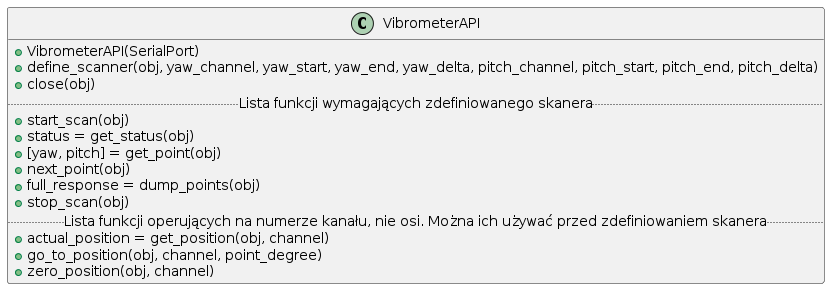
\includegraphics[width=\textwidth]{img/MatlabAPI_UML.png}
\caption{Diagram UML klasy sterującej systemem do pozycjonowania wibrometru.}
\label{img:matlab_api_uml}
\end{figure}


% \ref{lst:matlab_api_list}.
% \begin{lstlisting}[caption={Lista funkcji zaimplementowanych w API Matalb-owym},label={lst:matlab_api_list},style=Matlab,numbers=none]
% % Konstruktor:
% VibrometerAPI(SerialPort)

% % Funkcja definiująca skaner:
% define_scanner(obj, yaw_channel, yaw_start, yaw_end, yaw_delta, pitch_channel, pitch_start, pitch_end, pitch_delta)

% % Lista funkcji wymagających zdefiniowanego skanera:

% % Start skanowania, przemieszczenie do punktu startowego:
% start_scan(obj)
% % Pobranie statusu skanera:
% status = get_status(obj)
% %Pobranie obecnego, faktycznego punktu:
% [yaw, pitch] = get_point(obj)
% % Przemieszczenie do kolejnego punktu (pod warunkiem znajdowania się w stanie WaitingForNextPoint)
% next_point(obj)
% % Pobranie wszystkich punktów od początku pomiaru lub ostatniego wywołania tej komenda. Również przenosi skaner ze stanu Finished w stan Ready:
% full_response = dump_points(obj)
% % Przedwczesne przerwanie pomiaru:
% stop_scan(obj)

% % Lista funkcji pomocniczych, operujących na numerze kanału, nie osi. Można ich używać przed zdefiniowaniem skanera:

% % Zebranie faktycznej pozycji jednego z kanałów:
% actual_position = get_position(obj, channel)

% % Przejście na konkretną pozycję jednego z kanałów:
% go_to_position(obj, channel, point_degree)

% % Wyzerowanie pozycji kanału (Ustawienie obecnej pozycji jaki pozycji 0):
% zero_position(obj, channel)

% % Funkcja zamykająca połączenie portu szeregowego:
% close(obj)

% \end{lstlisting}


\subsection{Aplikacja GUI}
\label{cha:gui_app}
Dodatkowo, aby ułatwić manualną interakcję ze stołem, powstała aplikacja desktopowa z GUI, pozwalająca manualnie wywołać wszystkie dostępne operacje. Została napisana w języku C\#, frameworku Avalonia UI. Avalonia to open-sourcowy zestaw bibliotek, pozwalający pisać aplikacje cross-platformowe w języku C\#. Wspiera wszystkie wiodące systemy operacyjne, jak Windows, MacOS, Linux, Android czy iOS, ale także platforma ta podbija bardziej niszowe systemy, jak Tizen OS. Dodatkowo, poza aplikacjami na te systemy operacyjne, można napisać w nim stronę internetową, która będzie działać w większości wiodących przeglądarek internetowych. A co więcej, istnieje możliwość zbudowania jednego projektu dla wszystkich tych systemów, który wydziela wspólną część logiki programu. Jedynie system prezentacji danych jest różny dla różnych platform. Daje to możliwość zaoszczędzenia setek godzin pracy nad bliźniaczymi aplikacjami na różne systemy operacyjne. \cite{avalonia}

Na potrzeby tego projektu został natomiast wykorzystany jedynie ułamek możliwości tej platformy - ponieważ w ramach pracy powstała jedynie aplikacja na komputery z systemem Windows 7 lub nowszym.

Avalonia wspiera dwa schematy programowania. \textbf{Code-behind}, opierający się na podziale aplikacji na warstwę opisującą wygląd aplikacji, tzw. front-end oraz warstwę zawierającą odwołania (\textbf{callbacki}) od front-endu oraz logikę programu, tzw. back-end \cite{avalonia_CB}, oraz \textit{ReactiveUI}, implementujący wzorzec MVVM (\textbf{Model-View/View Model}). \cite{avalonia_MVVM} Wzorzec MVVM wprowadza dodatkową warstwę aplikacji pomiędzy back-end a front-end. We wzorcu tym logika programu jest zupełnie oddzielona od front-endu. Front-end, tutaj zwany \textbf{View}, jest jedynie samym opisem wyglądu aplikacji. Warstwa środkowa, czyli \textbf{View Model}, zawiera wszystkie odwołania od przycisków, kod aktualizujący odpowiednie wyświetlane wartości itp., jakie są potrzebne aby front-end był w stanie wejść w interakcję z back-endem. Na samym dole znajduje się back-end, tutaj zwany \textbf{Model}, gdzie znajduje się logika programu, zupełnie niezależna od reszty programu. Podejście to jest przede wszystkim bardzo przydatne w przypadku pisania aplikacji, które mają być kompilowane na wiele różnych platform.\cite{MVVMvsCB} W tej pracy, pomimo stosunkowej prostoty aplikacji, zdecydowano się na podejście MVVM, ponieważ daje to lepsze możliwości potencjalnej rozbudowy aplikacji w przyszłości. 


Aplikacja "VibrometerHostApp.exe", w celu zapewnienia większego komfortu użytkownikowi, została podzielona na 4 podstawowe ekrany, zgodnie z pewnymi grupami operacji jakie mogą być wykonywane przez użytkowników w jednym czasie.

\subsubsection{Ekran łączenia}
Ekran łączenia pozwala na wybór portu szeregowego z listy rozwijanej oraz połączenie się z wibrometrem na tym porcie. Dodatkowo zaimplementowane jest zabezpieczenie, blokujące połączenie z portem, na który podpięte jest coś innego niż stół - podczas próby łączenia sprawdzane są funkcje dostępne w urządzeniu. Jeżeli różnią się od funkcji wymaganych przez aplikację desktopową - połączenie jest odrzucane a użytkownik widzi kod błędu. Wygląd ekranu przedstawiony jest na zrzucie ekranu \ref{img:vib_host1}. Widać na nim efekt próby połączenia z urządzeniem na porcie "COM1"\, które nie jest stołem do pozycjonowania wibrometru. Użytkownik został poinformowany o tym przez aplikację Hostapp oraz nie została wykonana żadna kolejna akcja.

\begin{figure}[h!] 
\centering 
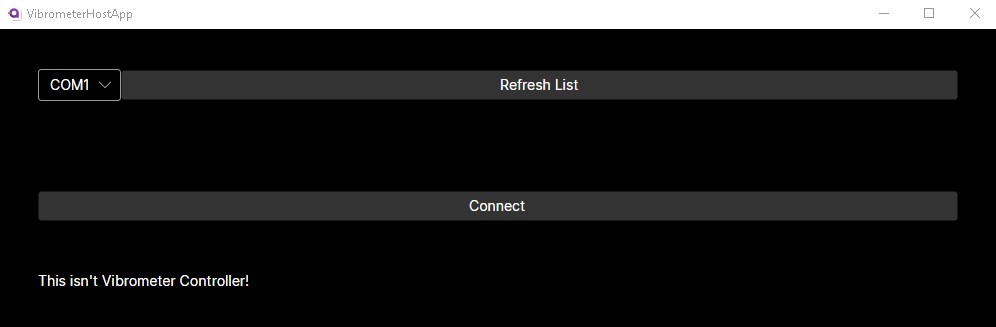
\includegraphics[width=\textwidth]{img/VibHost1.png}
\caption{Ekran łączności ze stołem do pozycjonowania.}
\label{img:vib_host1}
\end{figure}

\subsubsection{Ekran konfiguracyjny}
Kolejny jest ekran, pozwalający na konfigurację wibrometru - umożliwia on zdefiniowania 2 kanałów, yaw oraz pitch, w taki sam sposób jak definiowanie kanałów przy pomocy komend konsoli, lub API Matlab-owego. Po zdefiniowaniu obu kanałów można sprawdzić gotowość urządzenia i przejść do ekranu skanowania. W przypadku błędnej definicji kanałów, przycisk ready nie pozwoli przejść do kolejnego widoku. Wygląd ekranu przedstawiony jest na zrzucie ekranu \ref{img:vib_host2}. Widać na nim zdefiniowaną oś Yaw, wraz z pozytywną odpowiedzią od urządzenia, oraz jeszcze nie wypełnione wartości dla osi Pitch.

\begin{figure}[h!] 
\centering 
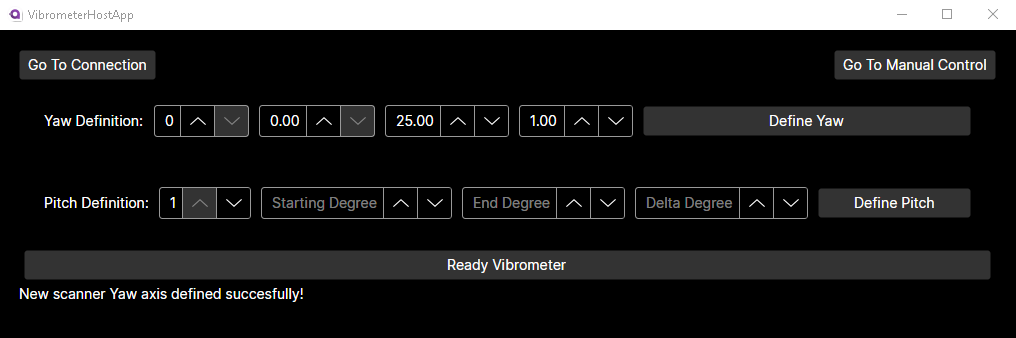
\includegraphics[width=\textwidth]{img/VibHost2.png}
\caption{Ekran konfiguracyjny stołu.}
\label{img:vib_host2}
\end{figure}

\subsubsection{Ekran skanowania}
Po udanym zdefiniowaniu osi skanowania wibrometru otwiera się ekran, dający możliwość kontroli nad samym procesem skanowania. Widać na nim takie przyciski, jak Start skanowania, Stop skanowania, zbieranie obecnego punktu, przemieszczanie się do kolejnego punktu, odczyt statusu oraz zrzut wszystkich odwiedzonych punktów. Przyciski te wykonują odpowiadające im komendy z konsoli, które opisane są rozdziale \ref{cha:commands}. Wygląd ekranu przedstawiony jest na zrzucie ekranu \ref{img:vib_host3}. Widać na nim skaner, który został przez użytkownika już uruchomiony, ponieważ zgłasza swój status jako WaitingForContinuation. Dodatkowo widać, że znajduje się na pozycji $1.35^{\circ}; 0.04^{\circ}$

\begin{figure}[h!] 
\centering 
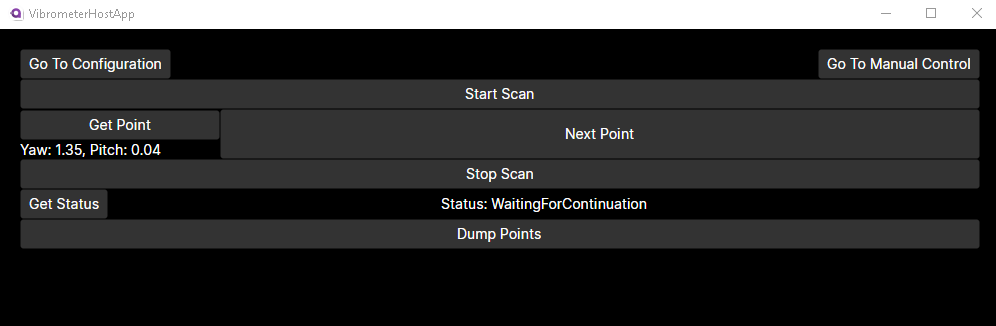
\includegraphics[width=\textwidth]{img/VibHost3.png}
\caption{Ekran skanowania.}
\label{img:vib_host3}
\end{figure}

\subsubsection{Ekran kontroli manualnej}
Podobnie jak w przypadku poprzednich form zarządzania urządzeniem, tutaj także jest dostęp do funkcjonalności zależnych jedynie od kanału, nie od zdefiniowanego skanera. Jednakże tutaj kontrola jest trochę większa niż w przypadku Matlaba - GUI daje dostęp do startowania i zatrzymywania silnika, oraz wysyłania silnika na konkretny kąt, wraz z odczytem obecnego kąta. Dodatkowo istnieje  możliwość wyzerowania pozycji - ustawienia obecnej pozycji jako kąt zerowy. Wygląd ekranu przedstawiony jest na zrzucie ekranu \ref{img:vib_host4}. Przedstawia on silnik na kanale 0 włączony i ustawiony na pozycji $10^{\circ}$. Natomiast silnik na kanale 1 jest wyłączony. Na przedstawionym zrzucie ekranu wyraźnie widać nieidealną precyzję kontroli pozycji - silnik został wysłany na kąt $10^{\circ}$, natomiast algorytm doprowadził go do pozycji $10.04^{\circ}$. 

\begin{figure}[h!] 
\centering 
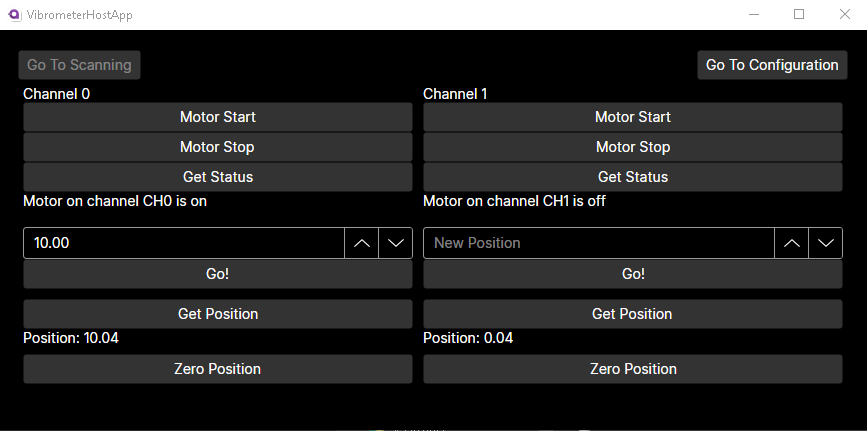
\includegraphics[width=\textwidth]{img/VibHost4.png}
\caption{Ekran kontroli manualnej.}
\label{img:vib_host4}
\end{figure}

Należy także wspomnieć o przyciskach do przechodzenia między ekranami. Każdy ekran zawiera dwa przyciski, w lewym i prawym górnym rogu. Pozwalają one na cofnięcie się do poprzednich ekranów, lub przejście do innego ekranu, który może być w danym momencie użytkownikowi potrzebny. W przypadku tego ekranu jest zaimplementowana blokada - nie da się przejść na ekran skanowania, jeżeli skaner nie jest zdefiniowany. Jest ona widoczna na zrzucie ekranu \ref{img:vib_host4}.

    \chapter{Pomiary wibrometrem skanującym}
\label{cha:Measurments}

W celu przetestowania powstałego urządzenia przeprowadzono pomiary wibracji blachy pod wpływem szumu białego. Celem pomiarów było stworzenie map w kolejnych tercjach. Każda mapa składała się z zestawu punktów, gdzie każdy punkt przedstawiał prędkość drgań blachy w danym punkcie pomiarowym.

\section{Stanowisko Pomiarowe}
Szum został wygenerowany przy pomocy generatora Bruel\&Kjaer 1405, wzmacniacza oraz głośnika znajdującego się w komorze pogłosowej Laboratorium Akustyki Technicznej. Natomiast, jako że wyjściem wibrometru jest sygnał ciągły dźwiękowy, do zebrania próbek sygnału użyto karty dźwiękowej. W celu zebrania pomiarów powstał skrypt w języku Matlab, który wchodził w interakcję zarówno z kartą dźwiękową, w celu zapisywania próbek dźwięku, oraz z systemem pozycjonowania powstałym w ramach tej pracy, w celu przemieszczania wibrometru. Opisywane stanowisko przedstawione jest na zdjęciu \ref{img:meas_setup}.

\begin{figure}[h!] 
\centering 
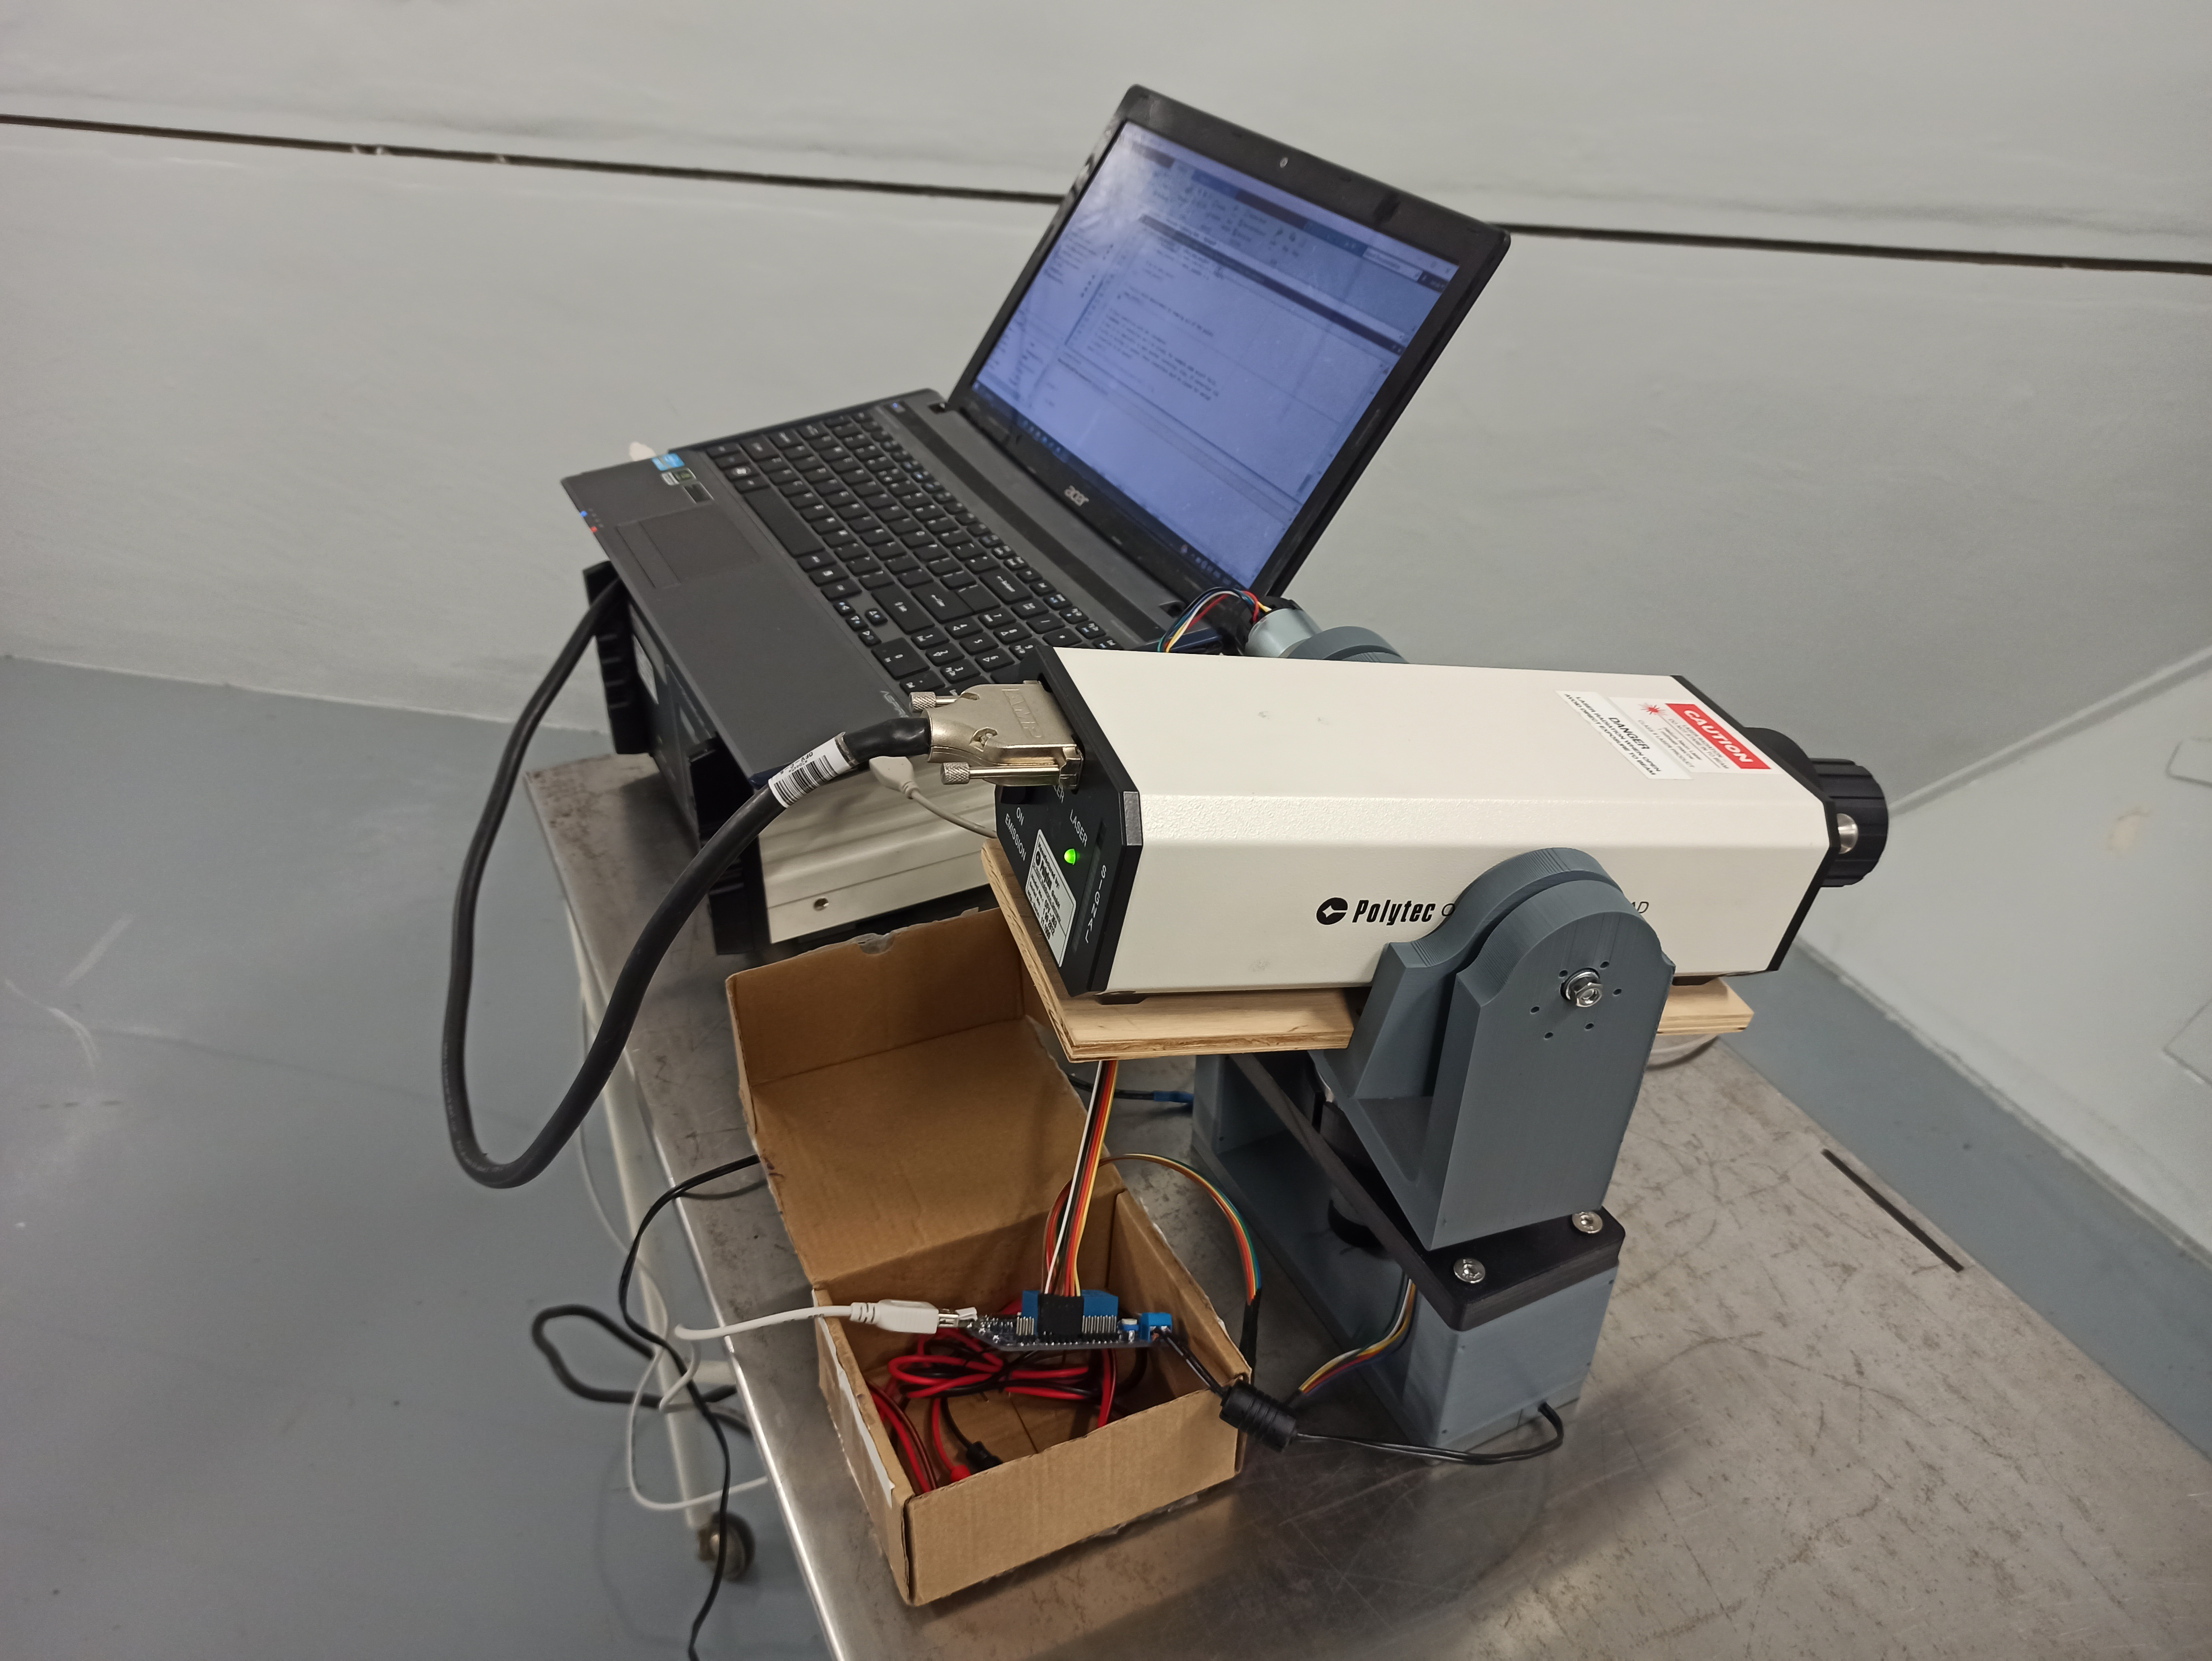
\includegraphics[width=0.6\textwidth]{img/MeasSetup.jpg}
\caption{Stanowisko pomiarowe.}
\label{img:meas_setup}
\end{figure}

\section{Algorytm zbierający dane}
Z kąta ustawienia metalowej płyty względem ziemi, odległości ustawienia wibrometru względem płyty, oraz zakresów ruchu wibrometru, wynikał zakres w jakim została płyta przeskanowana. Obrót dookoła osi yaw, czyli z, został ustawiony na zakres $\pm9^{\circ}$, co w odległości, w jakiej został ustawiony wibrometr, daje pełną szerokość płyty, czyli $40 cm$. Bardziej problematyczna była oś pitch, czyli obrót dookoła osi y. Ponieważ mierzona płyta była ustawiona pod kątem $50^{\circ}$ do podłoża, a wibrometr był w stanie zniżyć się maksymalnie o $30^{\circ}$. Oznaczało to, że pozycja w której wibrometr jest ustawiony poziomo jest odchylona od płaszczyzny pomiarowej o $40^{\circ}$. Dlatego też zdecydowano się na ustawienie zera relatywnego dla tej osi na kącie $20^{\circ}$, ponieważ wtedy laser celował w górę płyty, a zakres ruchu wibrometru ustalono na $0^{\circ}$-$10^{\circ}$, czyli o jeden stopień ponad połowę płyty. Natomiast na potrzeby późniejszych obliczeń zapisano wartość $-20^{\circ}$ jako przesunięcie pozycji zero tej osi wibrometru względem faktycznej osi prostopadłej do powierzchni blachy. Dokładny schemat przedstawiający ułożenie wibrometru w osi pitch znajduje się na rys \ref{img:pitch_schematic_drawing}. W tym miejscu można także zaznaczyć, że z punktu widzenia końcowego pomiaru nie ma znaczenia, czy jako oś zero zostanie ustalona faktyczna oś pozioma i późniejsze przesunięcie będzie wynosić $-40^{\circ}$ zamiast $-20^{\circ}$, czy zostanie to zrobione tak jak w przypadku tego pomiaru - oś zerowa zostanie przesunięta względem osi poziomej. Jest to wybór, który pozostaje w gestii osoby dokonującej pomiarów. Ważnym jest aby być świadomym kątów, pod jakimi zostały zbierane pomiary w celu późniejszej analizy danych.

\begin{figure}[h!] 
\centering 
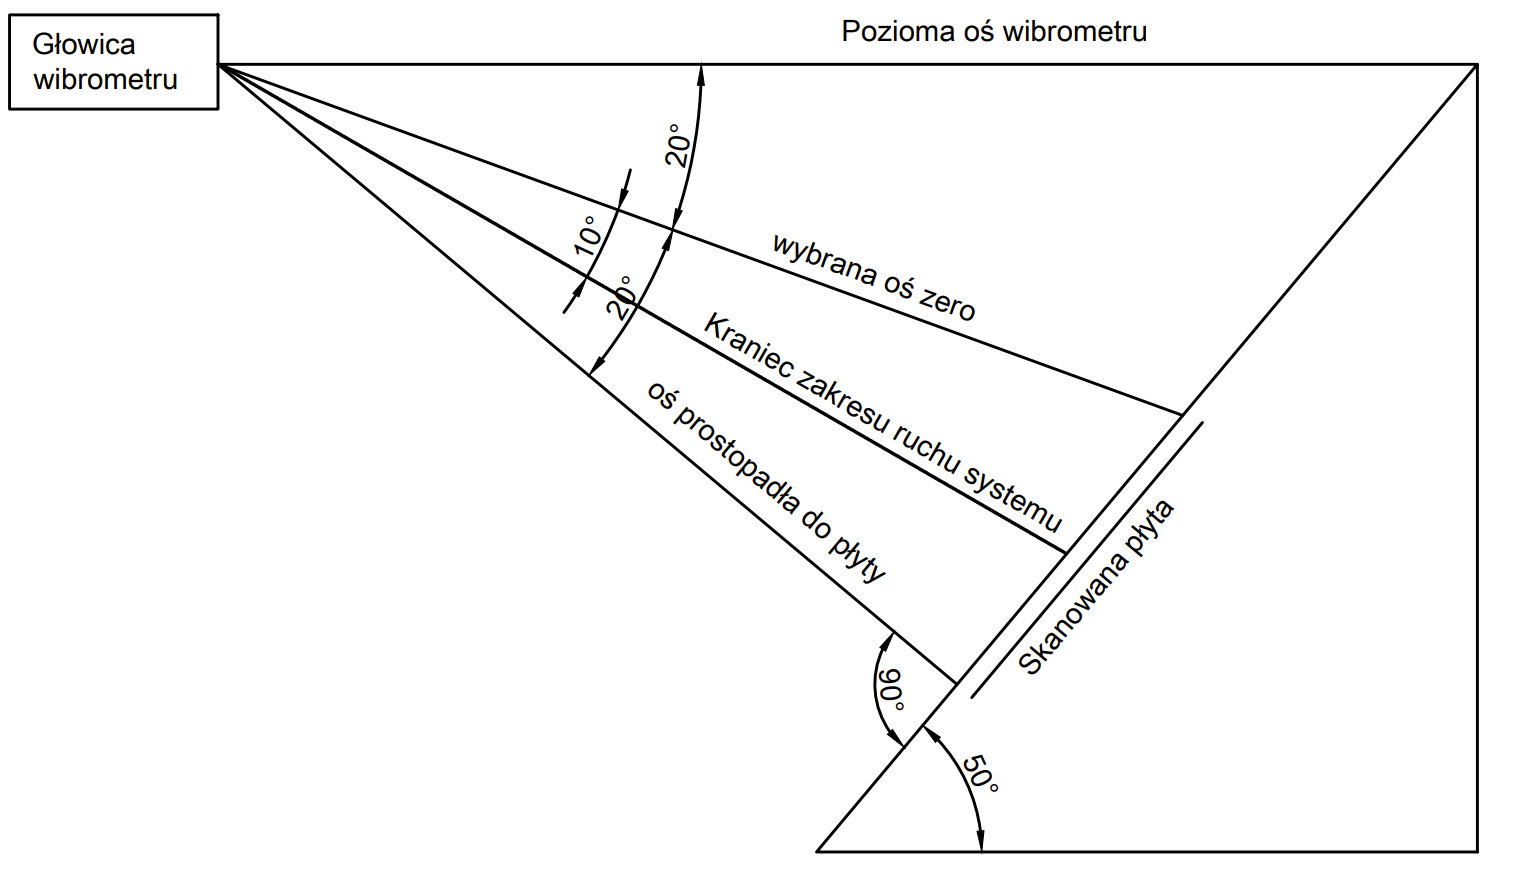
\includegraphics[width=\textwidth]{img/pitch_meas_schematic_draw.png}
\caption{Schemat ustawienia wibrometru w osi pitch.}
\label{img:pitch_schematic_drawing}
\end{figure}

Po inicjalizacji systemu, która jako argumenty przyjmuje właśnie powyższe wartości kątów, następuje pomiar w pętli, która trwa, dopóki system nie przejdzie w status Finished, kiedy to wykonywany jest ostatni pomiar oraz dane zapisywane są do pliku .mat. W każdym punkcie pomiarowym skrypt odczekuje $2s$, aby ustabilizować drgania wibrometru wynikające z plastikowej (drukowane w 3D) konstrukcji, oraz zbiera pięcio-sekundową ($5s$) próbkę dźwięku (używając metody \texttt{recordblocking()} z klasy \texttt{audiorecorder}), z częstotliwością próbkowania $8kHz$. Dodatkowo zapisywana jest dokładna pozycja wibrometru (używając metody \texttt{get\_point()} z klasy \texttt{VibrometerAPI}). Wszystkie te informacje zmierzone w punkcie zapisywane są do listy struktur, która to po skończonych pomiarach zapisywana jest do pliku .mat. Dokładny algorytm przedstawiony jest na schemacie \ref{img:matlab_data_acq_uml}.

\begin{figure}[h!] 
\centering 
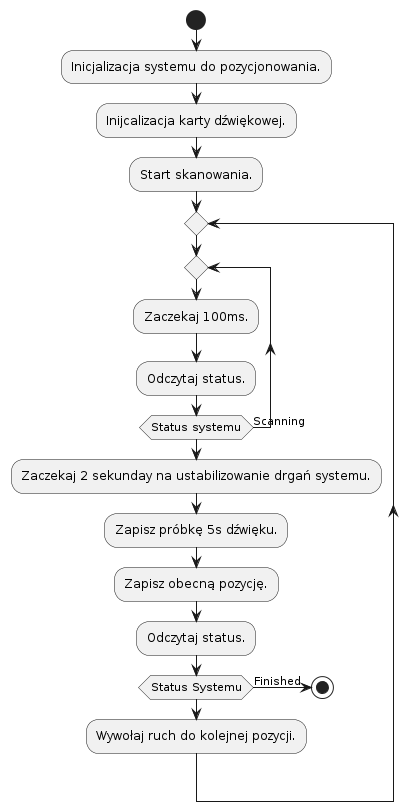
\includegraphics[width=0.7\textwidth]{img/MatlabDataAcq.png}
\caption{Uproszczony algorytm zbierający danych.}
\label{img:matlab_data_acq_uml}
\end{figure}



\section{Algorytm analizujący dane}
Algorytm analizujący dane jako swoje wejście wczytuje plik, zawierający  listę struktur ze wszystkimi zmierzonymi punktami, natomiast jego wyjściem jest zestaw wykresów, po jednym dla każdego analizowanego pasma częstotliwości.

\begin{figure}[h!] 
\centering 
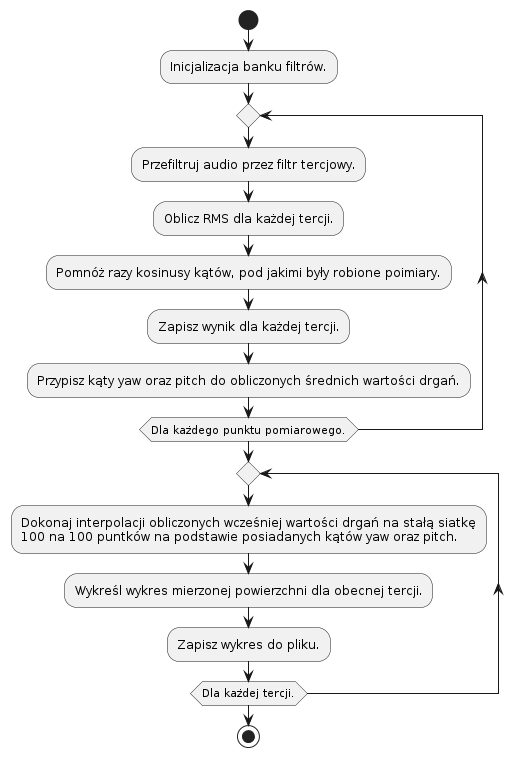
\includegraphics[width=0.7\textwidth]{img/AnalyseDataUML.png}
\caption{Algorytm analizy danych pomiarowych.}
\label{img:analyse_data_uml}
\end{figure}

Pierwszy krok algorytmu to iteracja po wszystkich odwiedzonych przez wibrometr punktach. W każdym punkcie należy rozbić sygnał na częstotliwości, w tym przypadku na tercje w zakresie $22Hz$ do $4kHz$, za pomocą filtru z klasy \texttt{octaveFilterBank}. W tym zakresie wspomniany filtr stworzył 26 tercji. Następnie, nadal w pętli po punktach, dla każdej z tych tercji, należy policzyć średnią za pomocą funkcji \texttt{rms}. Daje to średnią prędkość drgań danego punktu w danym zakresie częstotliwości. Kolejnym krokiem jest uwzględnienie faktu, że pomiar odbywał się pod kątem do powierzchni. Aby tego dokonać, obliczoną średnią energię należy pomnożyć razy cosinus kąta, pod jakim został dokonany pomiar, zarówno dla osi obrotu pitch jak i yaw. Należy także pamiętać o przesunięciu, czyli uwzględnieniu $-20^{\circ}$ dla osi pitch. Po wyjściu z pętli w odpowiednich zmiennych znajdują się informacje o średniej energii drgań we wszystkich tercjach oraz we wszystkich punktach. Dodatkowo, nadal istotna jest znajomość koordynatów tych punktów, aby poprawnie je zaznaczyć na wykresie. Ostatnim krokiem algorytmu jest pętla iterująca po 26 tercjach - dla każdej tercji należy przeprowadzić interpolację punktów oraz nakreślić je na wykresie. Dokładny algorytm znajduje się na schemacie \ref{img:analyse_data_uml}.



\section{Wyniki pomiarów}
W pierwszej kolejności zmierzono w kilku losowych punktach wartości drgań tła, czyli drgania bez włączonego głośnika. Przykładowo, wykres \ref{img:background_noise_graph} przedstawia drgania szumu w punkcie startowym równym $yaw = 0$ oraz $pitch = 0$. Wykres pokazuje, że w dolnych zakresach częstotliwości, wartości drgań są na poziomie części tysięcznych ($2 \cdot 10 ^ {-3}$), a w wyższych częstotliwościach schodzą nawet do części dziesięciotysięcznych ($5 \cdot 10 ^ {-4}$). W dalszych pomiarach wartości te będą stanowiły referencję, określającą czy wibrometr zbiera faktyczną wiązkę odbitą, czy zaledwie szumy tła.

\begin{figure}[h!] 
\centering 
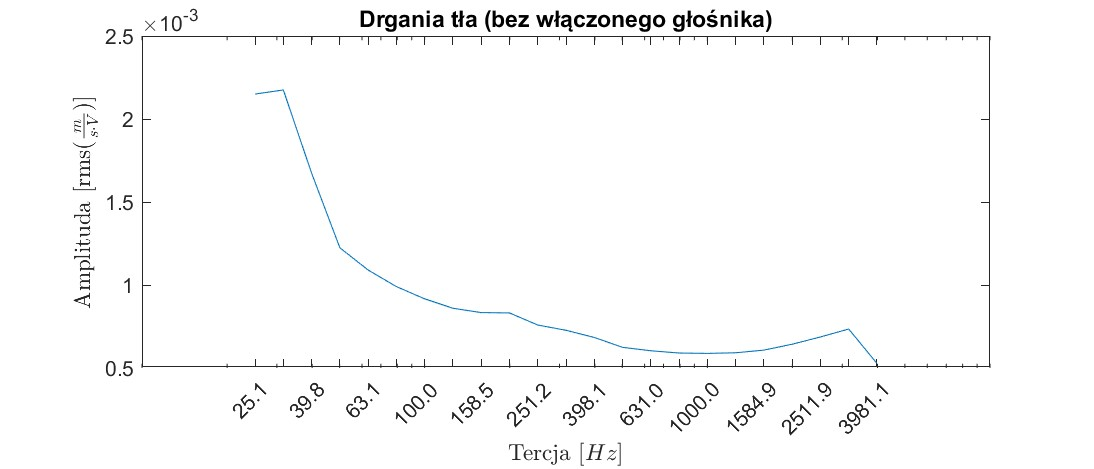
\includegraphics[width=\textwidth]{img/BackgroundGraph.jpg}
\caption{Szum drgań tła.}
\label{img:background_noise_graph}
\end{figure}

W drugiej kolejności wykonano opisywany wcześniej właściwy pomiar. Najmocniejsze drgania zarejestrowano dla tercji $31.6Hz$, ponieważ sięgały aż $0.22 \frac{m}{s \cdot V}$ na środku płyty, a $0.02 \frac{m}{s \cdot V}$ na rogach płyty. Jest to aż kolejno $100$ krotnie (dla środka płyty) oraz $10$ krotnie (dla brzegów płyty) więcej, niż zmierzone wcześniej tło. Rozkład drgań dla tercji $31.6Hz$ przedstawia wykres \ref{img:2_GraphThird}.

\begin{figure}[h!] 
\centering 
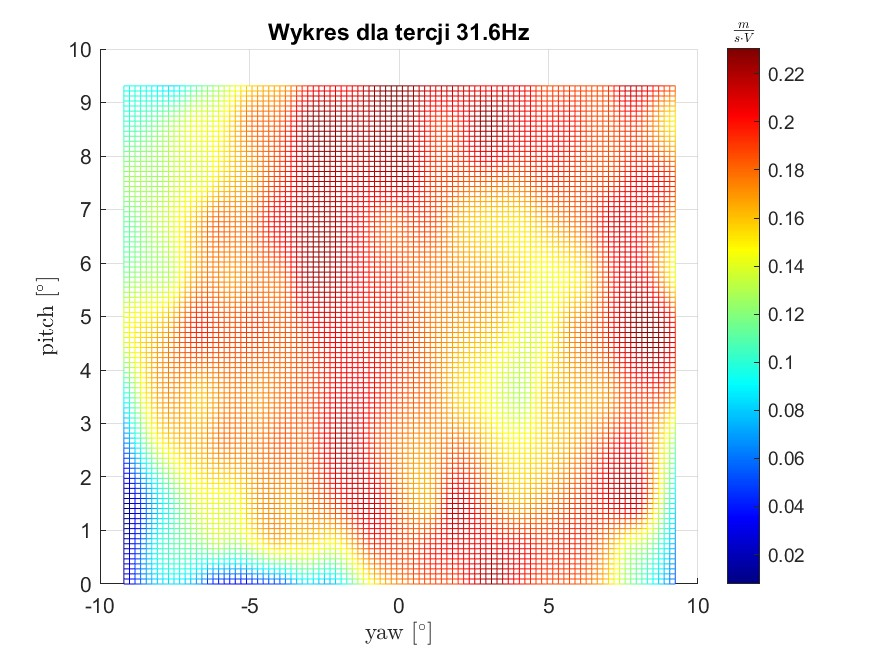
\includegraphics[width=0.8\textwidth]{img/2_GraphThird.jpg}
\caption{Rozkład drgań dla tercji $31.6Hz$.}
\label{img:2_GraphThird}
\end{figure}

Dla trzech pierwszych tercji, o częstotliwościach środkowych $25.1Hz$, $31.6Hz$, $39.8Hz$ nie widać żadnych wyraźnie zaznaczonych mod drgań. Natomiast w tercji o częstotliwości środkowej $50.1Hz$, widać wyraźnie zaznaczoną modę znajdującą się w lewej połówce badanej płyty. Wykres drgań płyty dla tej tercji przedstawia rysunek \ref{img:4_GraphThird}. Pokazuje on opisywany wyraźny wzrost prędkości drgań w lewej połówce płyty, blisko krawędzi. Porównując ten wykres z pozostałymi można także zauważyć ciekawe zjawisko. Płyta w tej częstotliwości drga dosyć intensywnie blisko krawędzi, pomimo że była ona przy krawędziach przytwierdzona do podłoża. Jest to także jedyna tercja, gdzie płyta drga intensywniej po lewej stronie, niż po prawej stronie. Natomiast biorąc pod uwagę, że pasta którą przytwierdzono płytę do podłoża nie była równomiernie rozłożona, oraz płyta nie była idealnie wypolerowana, zjawiska takie są oczekiwane.

\begin{figure}[h!] 
\centering 
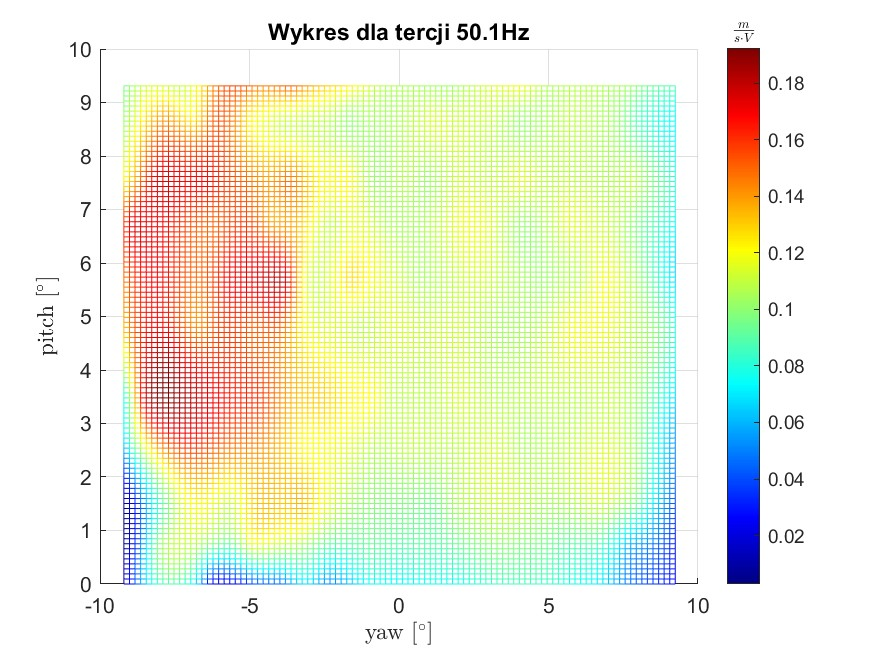
\includegraphics[width=0.8\textwidth]{img/4_GraphThird.jpg}
\caption{Rozkład drgań dla tercji $50.1Hz$.}
\label{img:4_GraphThird}
\end{figure}

Tak jak już wspomniano powyżej, tercja o częstotliwości środkowej $50.1Hz$ jest jedyna, gdzie drgania są wyraźniejsze po lewej stronie płyty. Już dla kolejnej tercji, o częstotliwości $63.1Hz$, widać wyraźne przesunięcie strzałki fali w prawą połówkę płyty. Rozkład drgań dla tercji $63.1Hz$ przedstawiony jest na wykresie \ref{img:5_GraphThird}. Podobne zachowania można zaobserwować także dla dwóch kolejnych tercji o częstotliwościach $79.4Hz$ oraz $100Hz$.

\begin{figure}[h!] 
\centering 
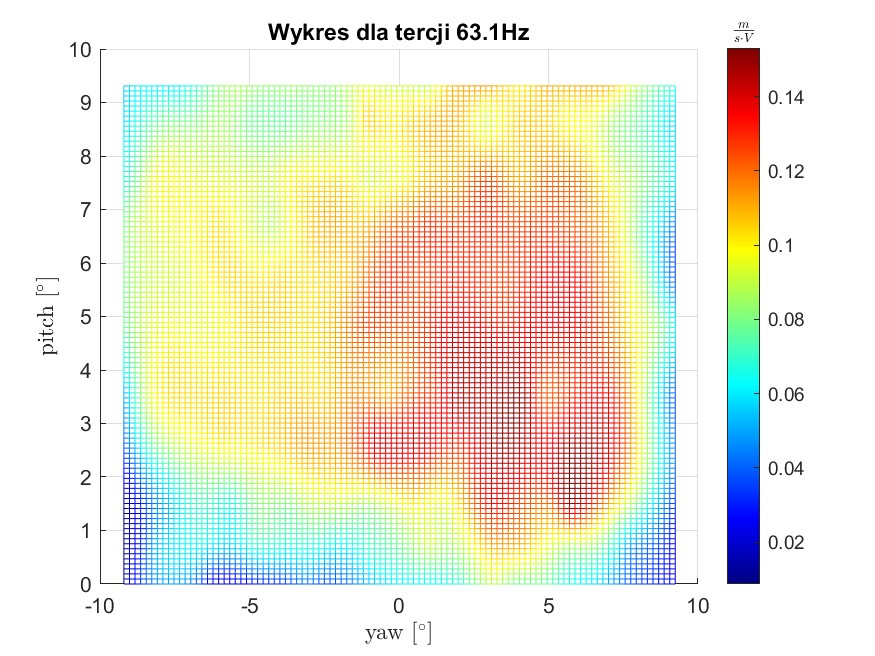
\includegraphics[width=0.8\textwidth]{img/5_GraphThird.jpg}
\caption{Rozkład drgań dla tercji $63.1Hz$.}
\label{img:5_GraphThird}
\end{figure}

Tak samo jak dla samego tła, amplituda drgań w wyższych częstotliwościach zaczyna zanikać dość gwałtownie. Przykładowo, dla tercji $125.9Hz$ widać wyraźny zanik drgań. Wysoka amplituda zachowała się jedynie w dwóch punktach. Rozkład drgań dla tej tercji przedstawia wykres \ref{img:8_GraphThird}. Natomiast już w kolejnej tercji, $158.5Hz$, także i te dwa punkty zanikają, co przedstawia wykres \ref{img:9_GraphThird}.

\begin{figure}[h!] 
\centering 
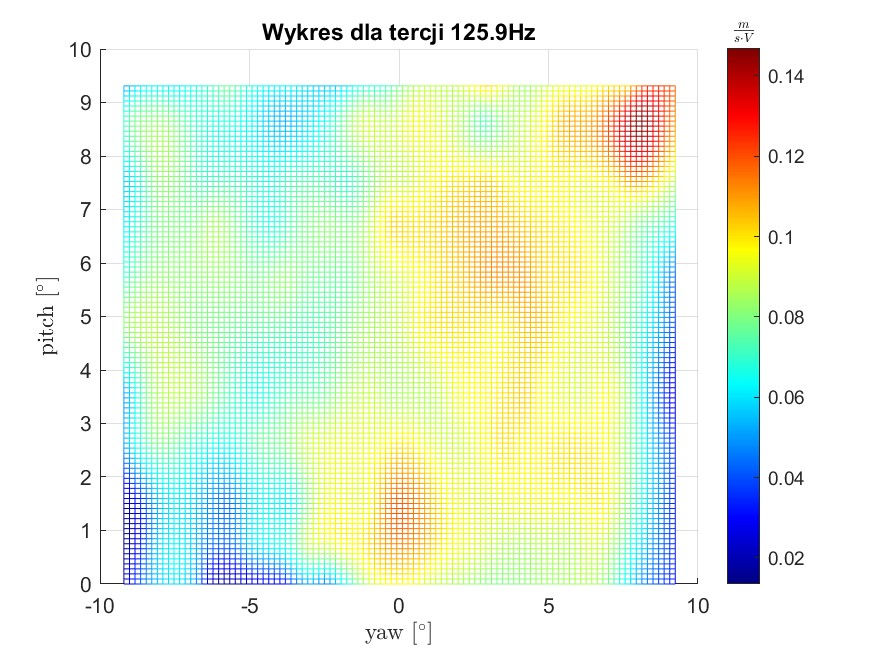
\includegraphics[width=0.8\textwidth]{img/8_GraphThird.jpg}
\caption{Rozkład drgań dla tercji $125.9Hz$.}
\label{img:8_GraphThird}
\end{figure}

\begin{figure}[h!] 
\centering 
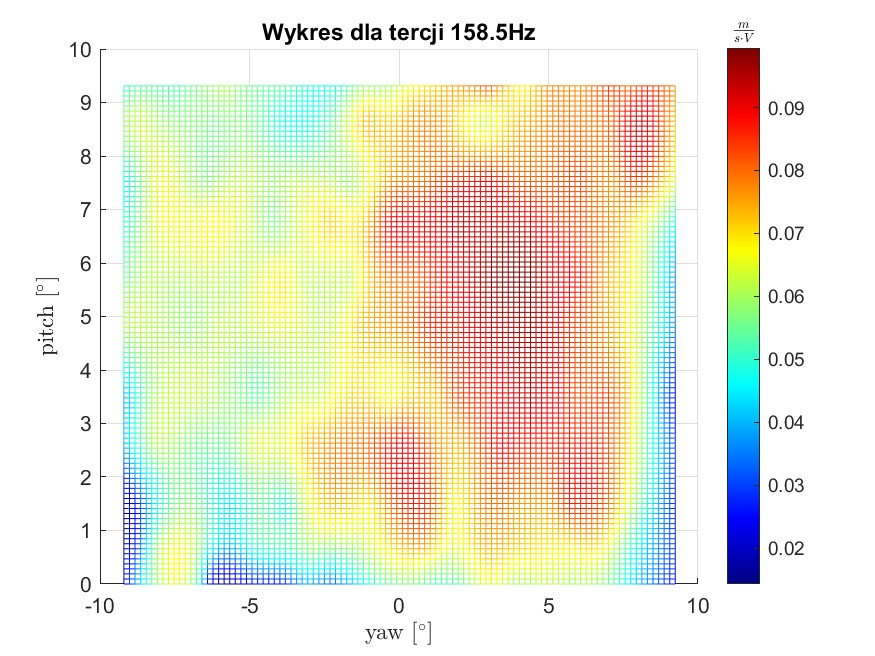
\includegraphics[width=0.8\textwidth]{img/9_GraphThird.jpg}
\caption{Rozkład drgań dla tercji $158.5Hz$.}
\label{img:9_GraphThird}
\end{figure}

Podobne zachowanie można zaobserwować poprzez wszystkie tercje o wyższych częstotliwościach środkowych. Wszędzie drgania są wyraźnie mocniejsze po prawej stronie płyty. Także zależnie od częstotliwości, albo cała prawa strona drga jednolicie, albo można nakreślić wyraźne punkty - strzałki drgań - w których drgania są zdecydowanie mocniejsze. Pomimo że następuje też statyczny spadek amplitudy drgań, i dla częstotliwości $4kHz$ drgania są już na poziomie zaledwie $10^{-2}$-$10^{-3}$, to należy pamiętać wykres \ref{img:background_noise_graph}, gdzie dla tych częstotliwości poziom szumów tła spadł do poziomu $5 \cdot 10^{-4}$, co oznacza, że nawet najsłabsze drgania dla tych częstotliwości, przy włączonym głośniku są nadal 20-krotnie wyższe niż przy głośniku wyłączonym. Rozkład drgań dla opisywanej częstotliwości opisuje wykres \ref{img:23_GraphThird}.

\begin{figure}[h!] 
\centering 
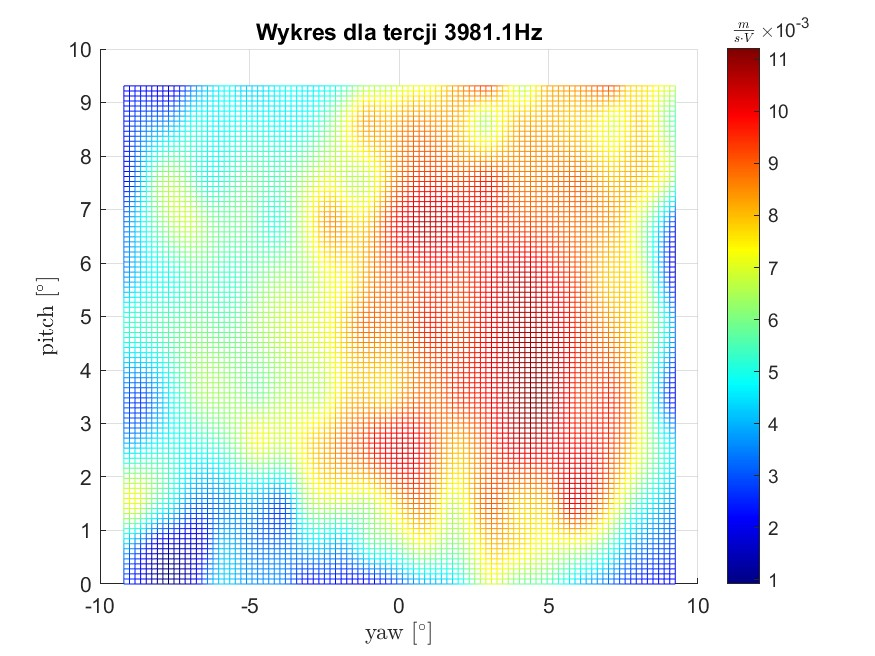
\includegraphics[width=0.8\textwidth]{img/23_GraphThird.jpg}
\caption{Rozkład drgań dla tercji $4kHz$.}
\label{img:23_GraphThird}
\end{figure}
    \chapter{Wnioski}
\begin{figure}[h!] 
\centering 
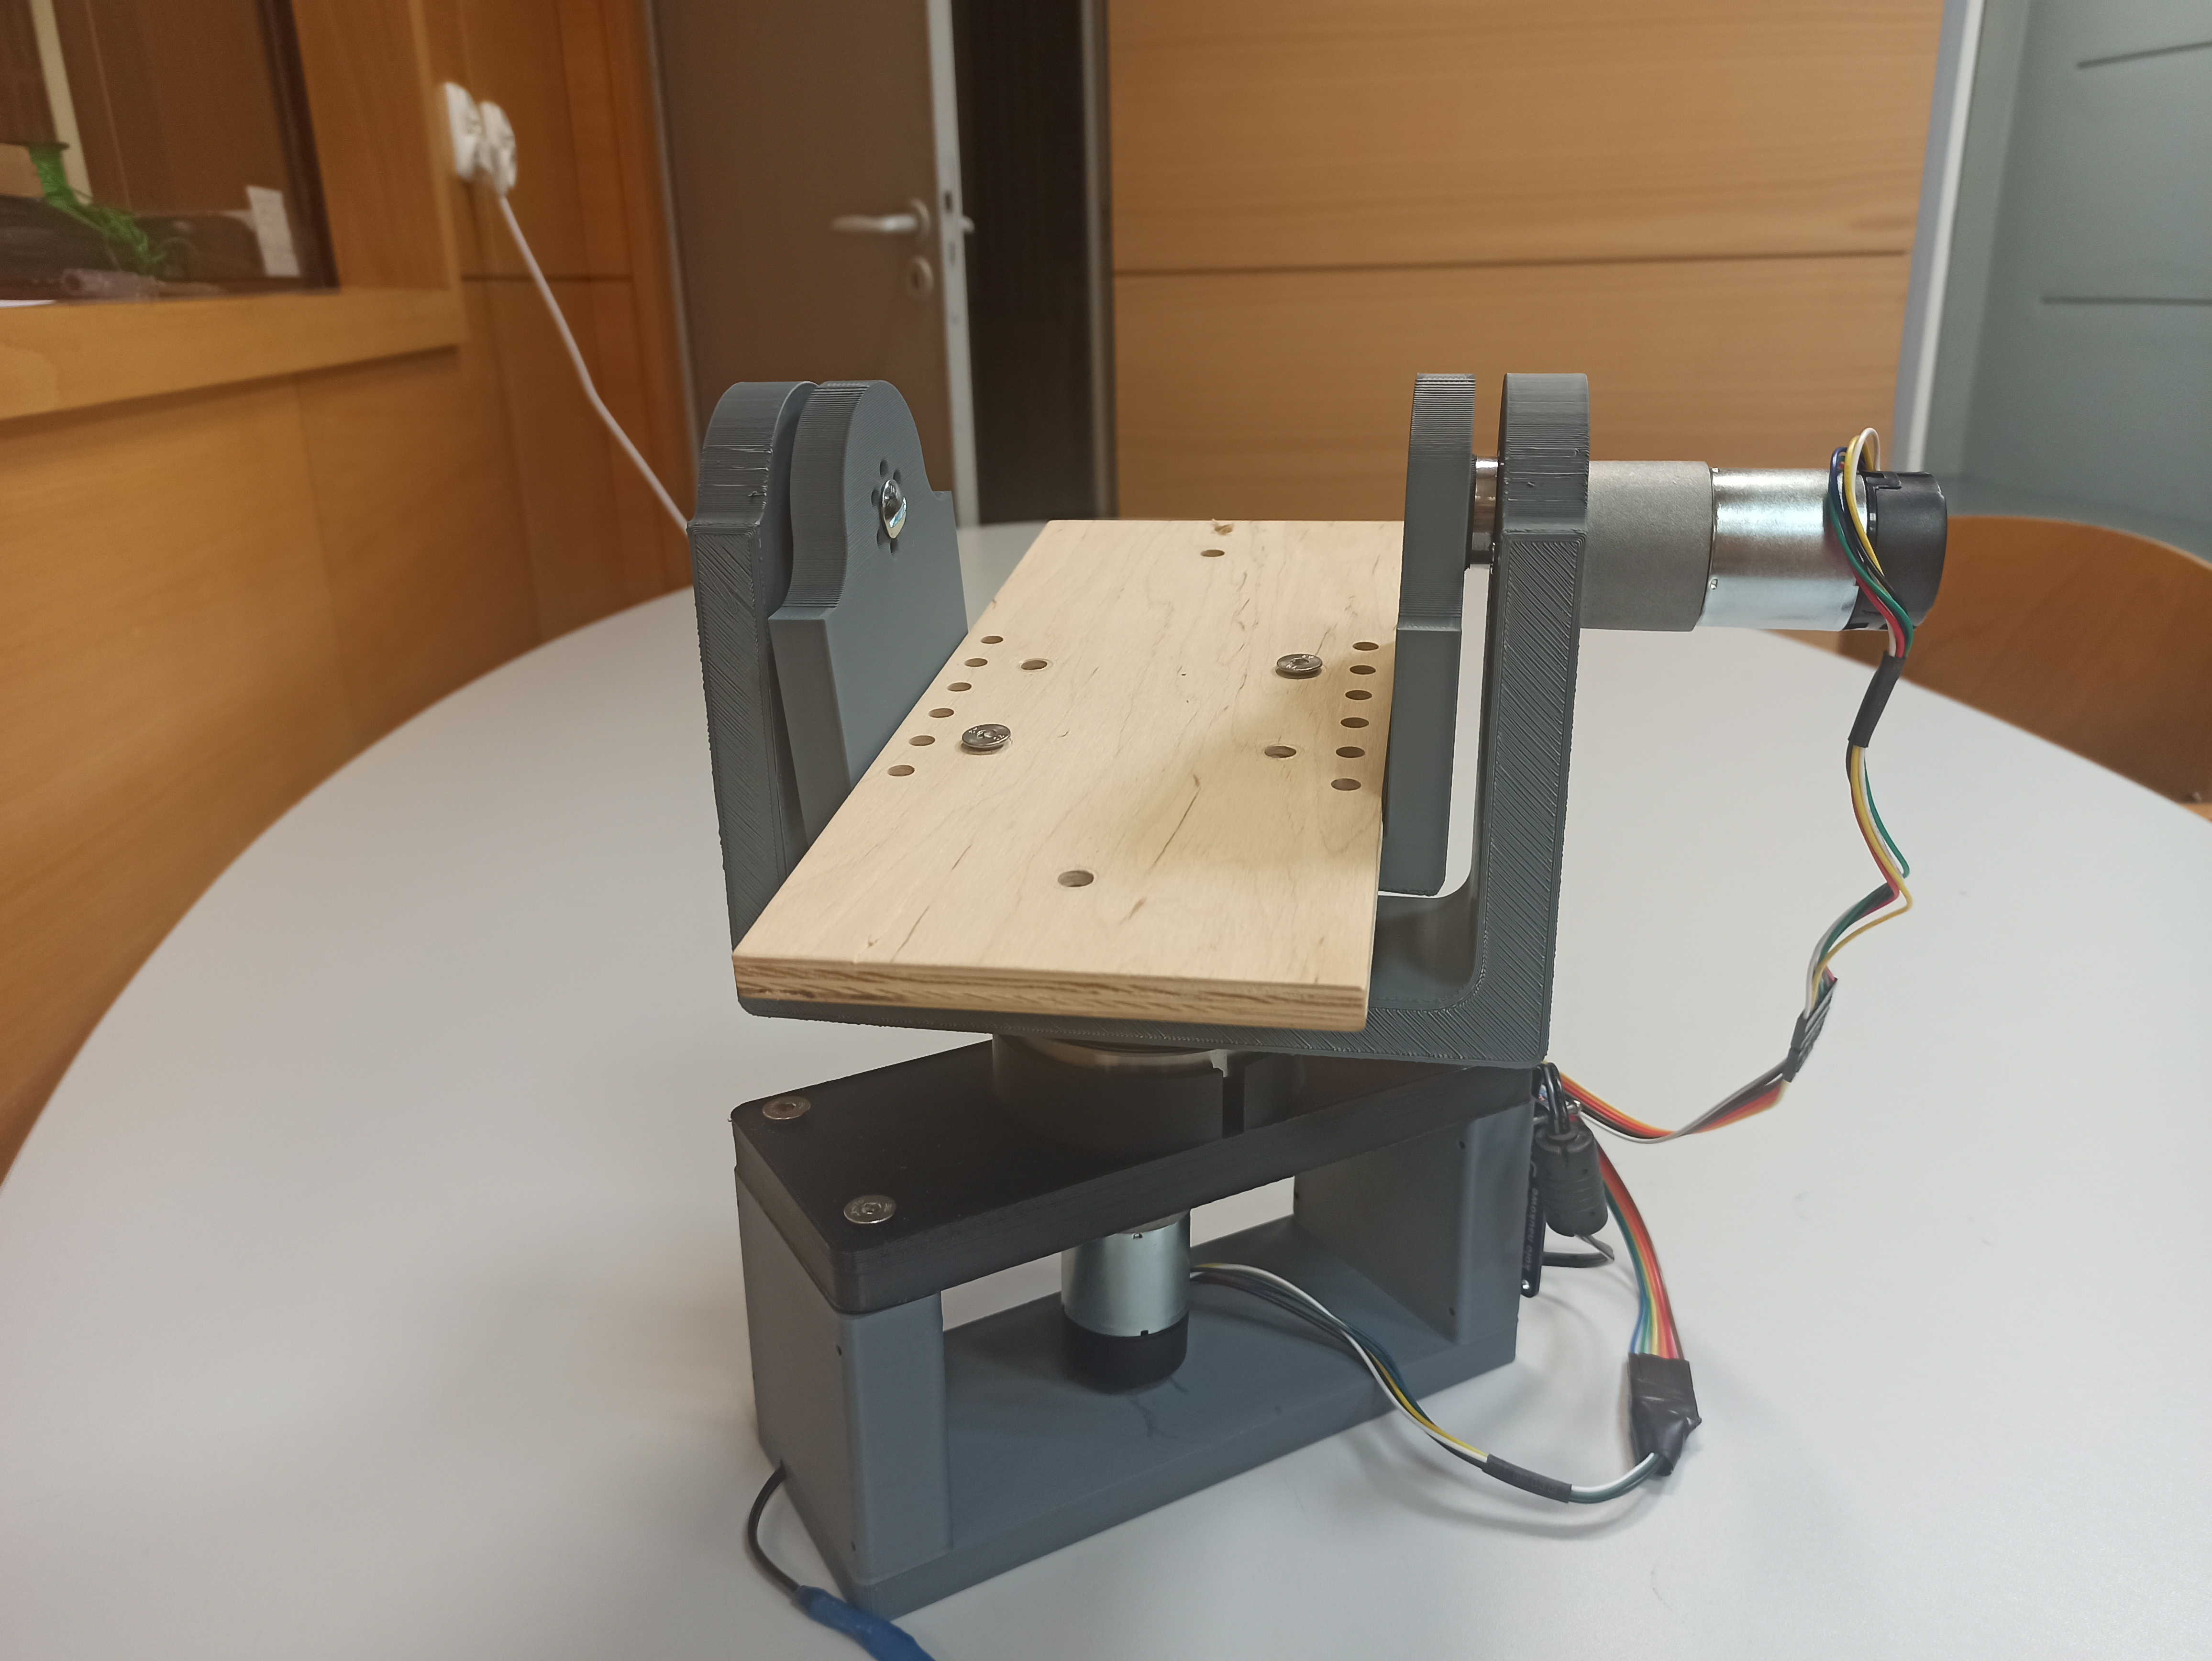
\includegraphics[width=\textwidth]{img/systemPhoto.jpg}
\caption{Skonstruowany system.}
\label{img:systemPhoto}
\end{figure}

Zaprezentowane w rozdziale \ref{cha:Measurments} pomiary, pokazują, że zbudowane urządzenie, przedstawione na zdjęciu \ref{img:systemPhoto}, działa poprawnie. Celem pracy było przeskanowanie powierzchni przy pomocy wibrometru punktowego  i cel ten został osiągnięty.

Oprogramowanie działa bez zarzutu oraz zgodnie z opisem przedstawionym w ramach tej pracy. Przy wielokrotnym uruchamianiu i podczas wykonywania wielu skanów nie wykazało żadnych błędów. Natomiast należy pamiętać, że zgodnie z teorią testowania oprogramowania, można jedynie wykazać istnienie błędów, nie można udowodnić ich braku. Dlatego też sugeruje się, aby podczas wykonywania pomiarów przymocowywać system do podłoża, tak jak zostało to zrobione podczas pomiarów opisywanych w rozdziale \ref{cha:Measurments}. Wibrometr, nawet punktowy, jest bardzo drogim urządzeniem, a przy gwałtownych ruchach spowodowanych błędami oprogramowania lub sprzętu, cała konstrukcja może się przewrócić. Zwłaszcza, że środek masy wibrometru znajduje się wyżej, niż zakładano podczas tworzenia pierwszych wersji modeli, co spowodowało, że podstawa całego systemu jest za mała. Podczas normalnej pracy rozmiar postawy jest w zupełności wystarczający, natomiast w razie pojawienia się większych momentów istnieje ryzyko przesunięcia środka masy poza obszar podstawy i przewrócenie się urządzenia.

W tym miejscu można także zastanowić się nad sensem użycia silników szczotkowy w tego typu projekcie. System zadziałał, więc wydaje się to zasadne. Natomiast nie było to łatwe zadanie, regulator opisywany w rozdziale \ref{cha:pos_control} ostatecznie zawierał więcej elementów i wykonywał więcej obliczeń, jak na przykład histereza czy tandem dwóch regulatorów. Kontrola pozycji okazała się także mniej precyzyjna niż pierwotnie zakładano. Pomimo dużej precyzji enkodera, i dość dokładnej (bo do około $\pm0.05^{\circ}$) znajomości pozycji, to wymuszanie takiej dokładności powodowało znaczne przeregulowania, spowodowane faktem, że silnik szczotkowy ma pewną minimalną prędkość i nie da się go zmusić do wolniejszego ruchu. Dlatego też nawet najlepiej dostrojone regulatory mogłyby mieć problem z przeregulowaniem. W celu poprawienia tej regulacji można by podjąć próbę zaimplementowania regulatora w samym przerwaniu od enkodera, zamiast przerwaniu od zegara. Sprawiłoby to, że informacja o sprzężeniu zwrotnym byłaby natychmiastowa. Jednakże istnieje ryzyko, że procesor nie dałby rady wykonywać tylu obliczeń w tak krótkich odstępach czasu. Można by także spróbować użyć trybu "Short Brake", udostępnianego przez użyty sterownik Toshiby. Jednakże tryb ten powoduje gwałtowne hamowanie, co znowu mogłoby spowodować inne problemy, jak na przykład pękające zębatki przekładni. Alternatywnym, najprostszym rozwiązaniem byłoby zastąpienie silnika szczotkowego silnikiem krokowym, w przypadku którego takie problemy nie występują.

Kolejnym problemem jaki wyniknął z użycia silników szczotkowych to luzy. Bardzo możliwe że są one wywołane przez przekładnię, a nie sam silnik, więc nie da się jednoznacznie określić czy zastosowanie silników krokowych rozwiązałoby problem.

Podczas wykonywania pomiarów pojawił się także problem trzęsących się modeli. Jest to przypadłość materiałów, z jakich modele te zostały wydrukowane, są one dość giętkie. Dlatego też istotnym krokiem w dalszym rozwoju tego projektu byłoby wycięcie całości konstrukcji z aluminium, zamiast druku.

Potencjalne miejsce, gdzie można by rozwinąć oprogramowanie, zostało opisane w rozdziale \ref{cha:auto_scanner}. Zaznaczono tam potencjał dołączenia układu ADC, który zbierałby pomiary, zamiast dodatkowej karty dźwiękowej podpinanej do komputera. Idąc krok dalej, można by także przeprowadzić całą analizę danych po stronie mikrokontrolera, jednakże to wymagałoby implementacji całej filtracji oktawowej w języku C. Wykonanie tego zadania umożliwiłoby przeprowadzanie całych pomiarów za pomocą zaledwie jednej komendy wysyłanej do urządzenia. Kolejny aspekt potencjalnej rozbudowy, to komunikacja między wibrometrem a systemem pozycjonowania. Wibrometr posiada gniazdo RS-232. Zapoznanie się z komendami, pozwoliłoby na kontrolę wibrometru z poziomu powstałego systemu.

	
	% itd.
	% \appendix
	% \chapter{Lista opracownych skryptów i programów}
W ramach pracy powstało następująca lista oprogramowania. Wszystkie wspomniane pliki, wraz z pełnym kodem źródłowym oraz opublikowanymi, skompilowanymi programami są dołączone jako załączniki do pracy:
\section{Kod Embedded}
\begin{itemize}
    \item Rozbudowa sterownika do silników szczotkowych:
    \begin{itemize}
        \item \textbf{driver.c} oraz \textbf{driver.h} - pliki, w ramach których wykonywane są przerwania, od zegara oraz pinów enkodera, wraz z funkcjami ustawiającymi oraz odczytującymi parametry sterownika, jak obecna pozycja, nowa pozycja czy kierunek obrotu.
        \item \textbf{calculations.h} - plik towarzyszący, definiujący regulatory PID oraz zawierający dodatkowe makra kalkulacyjne.
    \end{itemize}
    \item Skaner:
    \begin{itemize}
        \item \textbf{scan\_driver.c} oraz \textbf{scan\_driver.h} - Pliki definiujące główny algorytm przechodzący po punktach w których ma się odbyć skanowanie.
        \item \textbf{scan\_buffer.c} oraz \textbf{scan\_buffer.h} - Pliki definiujące bufor, w którym zapisywane są kolejne odwiedzone punkty.
        \item \textbf{scan\_adc.c} oraz \textbf{scan\_adc.h} - pliki uruchamiające przetwornik cyfrowo analogowy, który stanowi podstawę potencjalnej rozbudowy projektu.
        \item \textbf{scan\_uart.c} - Plik definiujący obsługę USB, pozwalający na komunikację ze sterownikiem za pomocą szeregowych komend powłoki (serial shell).
        \item \textbf{scan\_return\_codes.h} - Plik definiujący kody odpowiedzi funkcji, w tym kody błędów.
        \item \textbf{main.c} - Plik zawierajćy kod odpowiedzialny za inicjalizację całego urządzenia i wszystkich jego funkcjonalności.
    \end{itemize}
    \item Pliki te, wraz z bibliotekami zephyr-a w wersji 2.6.0, kompilowane są za pomocą kompilatora GNU 12.2.0 do pojedynczego pliku \textbf{zephyr.hex}, który wgrywany jest na procesor. Do pracy dołączono ten plik w wersji sterownika 2.5 oraz skanera 1.0. Potencjalne nowsze wersje pliku, wraz z pełnym kodem źródłowym, będą znajdować się na repozytorium \href{https://github.com/eSqadron/Vibrometer-Positioning-Table}{Vibrometer Positioning Table}.
\end{itemize}
\section{API Matlaba}
\label{appendix:maltalb_api}
\begin{itemize}
    \item \textbf{VibrometerAPI.m} - plik definiujący klasę \texttt{VibrometerAPI}, pozwalającą na łączenie z systemem.
    \item \textbf{go\_to\_point\_sample.m} - skrypt, przedstawiający przykład ręcznego ustalenia nowego punktu, dojście do niego, oraz jego wyzerowanie.
    \item \textbf{collect\_data\_sample.m} - skrypt, przedstawiający przykład kompletnego procesu skanowania, wraz z zapisywaniem próbek dźwięku w każdym punkcie. Skrypt ten został użyty podczas pomiarów wykonanych w rozdziale \ref{cha:Measurments}.
    \item \textbf{analyze\_data\_sample.m} - skrypt, przedstawiający przykładową analizę danych zebranych podczas pomiarów. Skrypt ten został użyty podczas pomiarów wykonanych w rozdziale \ref{cha:Measurments}.
    \item \textbf{collect\_background\_sample.m} - skrypt, pozwalający na zebranie oraz prezentację danych z wibrometru w jednym, wcześniej ustalonym punkcie. Skrypt ten został użyty do oszacowania wibracji tła podczas pomiarów wykonanych w rozdziale \ref{cha:Measurments}.
\end{itemize}
\section{C\# Hostapp}
\begin{itemize}
    \item Modele:
    \begin{itemize}
        \item \textbf{Channel.cs} - Plik zawierający definicję numerów kanałów.
        \item \textbf{ScannerChannelDefinition.cs} - Plik zawierający opis pojedynczego kanału.
        \item \textbf{VibrometerConnection.cs} - Plik zawierający klasę singletonu odpowiadającego za główny opis połączenia z urządzeniem za pomocą komunikacji szeregowej.
        \item \textbf{VibrometerException.cs} - plik zawierający definicję wyjątków, rzucanych przez program.
    \end{itemize}
    \item Widoki i odpowiadające im modele widoków:
    \begin{itemize}
        \item \textbf{MainWindowViewModel.cs}, \textbf{MainWindow.axaml}, \textbf{MainWindow.axaml.cs} - Pliki zawierające definicję głównego okna, w którym wyświetlane są widoki.
        \item \textbf{ConnectionViewModel.cs}, \textbf{ConnectionView.axaml}, \textbf{ConnectionView.axaml.cs} - Pliki definiujące widok połączenia, oraz zachowanie tego widoku.
        \item \textbf{ConfigureViewModel.cs}, \textbf{ConfigureView.axaml}, \textbf{ConfigureView.axaml.cs} - Pliki definiujące widok konfiguracji urządzenia, oraz zachowanie tego widoku.
        \item \textbf{ScanningViewModel.cs}, \textbf{ScanningView.axaml}, \textbf{ScanningView.axaml.cs} - Pliki definiujące widok skanowania powierzchni przez urządzenie, oraz zachowanie tego widoku.
        \item \textbf{ManualControlViewModel.cs}, \textbf{ManualControlView.axaml}, \textbf{ManualControlView.axaml.cs} - Pliki definiujące widok manualnej kontroli nad urządzeniem, oraz zachowanie tego widoku.
    \end{itemize}
    \item Wszystkie powyższe pliki kompilowane są do pliku \textbf{VibrometerHostApp.exe}, wraz z towarzyszącymi plikami .dll. Powstały plik .exe wykonywalny jest na systemach z oprogramowaniem Windows 10 lub nowszym.
\end{itemize}

	% \chapter{Lista modeli 3D}
W ramach pracy powstały następujące modele 3D:
\begin{itemize}
    \item \textbf{VibrometerPositioningTable.f3d} -- Główne złożenie całego stołu do pozycjonowania wibrometru.
    \item Dolna, stacjonarna część stołu:
    \begin{itemize}
        \item \textbf{StaticBase.f3d} -- Cześć podtrzymująca dolne łożysko, do której przymocowany jest silnik.
        \item  \textbf{DownTable.f3b} -- Część która pozwala na montaż na stojaku mikrofonowym z gwintem \textbf{M6}.
        \item  \textbf{BaseSpacer.f3b} -- Część łącząca \textbf{StaticBase} oraz \textbf{DownTable}, dająca przestrzeń na montaż silnika.
    \end{itemize}
    \item Środkowa część stołu, poruszająca się w jednej osi.
    \begin{itemize}
        \item \textbf{PartialMovementTable.f3d} -- Część stołu, która porusza się dookoła osi z. Dodatkowo zawiera otwory, aby przymocować statyczną część drugiego silnika.
        \item \textbf{HubSpacer2.f3b} \& \textbf{HubSpcer5.f3b} -- Modele, które razem z hubem montażowym Pololu 1083 tworzą sprzęgiełko łączące \textbf{PartialMovementTable} wraz z dolnym silnikiem.
    \end{itemize}
    \item Górna część stołu, która wraz z wibrometrem obraca się dookoła obu osi.
    \begin{itemize}
        \item \textbf{Holder1.f3d} \& \textbf{Holder2.f3d} -- Dwie części, jedna montowalna do wału drugiego silnika, druga bezpośrednio na łożysko kulkowe.
        \item \textbf{PlywoodPlate.f3d} -- Cześć łącząca holdery do właściwej głowicy wibrometru.
    \end{itemize}
    
\end{itemize}
	% itd.
	
	\printbibliography

    \appendix
    \chapter{Lista opracownych skryptów i programów}
W ramach pracy powstało następująca lista oprogramowania. Wszystkie wspomniane pliki, wraz z pełnym kodem źródłowym oraz opublikowanymi, skompilowanymi programami są dołączone jako załączniki do pracy:
\section{Kod Embedded}
\begin{itemize}
    \item Rozbudowa sterownika do silników szczotkowych:
    \begin{itemize}
        \item \textbf{driver.c} oraz \textbf{driver.h} - pliki, w ramach których wykonywane są przerwania, od zegara oraz pinów enkodera, wraz z funkcjami ustawiającymi oraz odczytującymi parametry sterownika, jak obecna pozycja, nowa pozycja czy kierunek obrotu.
        \item \textbf{calculations.h} - plik towarzyszący, definiujący regulatory PID oraz zawierający dodatkowe makra kalkulacyjne.
    \end{itemize}
    \item Skaner:
    \begin{itemize}
        \item \textbf{scan\_driver.c} oraz \textbf{scan\_driver.h} - Pliki definiujące główny algorytm przechodzący po punktach w których ma się odbyć skanowanie.
        \item \textbf{scan\_buffer.c} oraz \textbf{scan\_buffer.h} - Pliki definiujące bufor, w którym zapisywane są kolejne odwiedzone punkty.
        \item \textbf{scan\_adc.c} oraz \textbf{scan\_adc.h} - pliki uruchamiające przetwornik cyfrowo analogowy, który stanowi podstawę potencjalnej rozbudowy projektu.
        \item \textbf{scan\_uart.c} - Plik definiujący obsługę USB, pozwalający na komunikację ze sterownikiem za pomocą szeregowych komend powłoki (serial shell).
        \item \textbf{scan\_return\_codes.h} - Plik definiujący kody odpowiedzi funkcji, w tym kody błędów.
        \item \textbf{main.c} - Plik zawierajćy kod odpowiedzialny za inicjalizację całego urządzenia i wszystkich jego funkcjonalności.
    \end{itemize}
    \item Pliki te, wraz z bibliotekami zephyr-a w wersji 2.6.0, kompilowane są za pomocą kompilatora GNU 12.2.0 do pojedynczego pliku \textbf{zephyr.hex}, który wgrywany jest na procesor. Do pracy dołączono ten plik w wersji sterownika 2.5 oraz skanera 1.0. Potencjalne nowsze wersje pliku, wraz z pełnym kodem źródłowym, będą znajdować się na repozytorium \href{https://github.com/eSqadron/Vibrometer-Positioning-Table}{Vibrometer Positioning Table}.
\end{itemize}
\section{API Matlaba}
\label{appendix:maltalb_api}
\begin{itemize}
    \item \textbf{VibrometerAPI.m} - plik definiujący klasę \texttt{VibrometerAPI}, pozwalającą na łączenie z systemem.
    \item \textbf{go\_to\_point\_sample.m} - skrypt, przedstawiający przykład ręcznego ustalenia nowego punktu, dojście do niego, oraz jego wyzerowanie.
    \item \textbf{collect\_data\_sample.m} - skrypt, przedstawiający przykład kompletnego procesu skanowania, wraz z zapisywaniem próbek dźwięku w każdym punkcie. Skrypt ten został użyty podczas pomiarów wykonanych w rozdziale \ref{cha:Measurments}.
    \item \textbf{analyze\_data\_sample.m} - skrypt, przedstawiający przykładową analizę danych zebranych podczas pomiarów. Skrypt ten został użyty podczas pomiarów wykonanych w rozdziale \ref{cha:Measurments}.
    \item \textbf{collect\_background\_sample.m} - skrypt, pozwalający na zebranie oraz prezentację danych z wibrometru w jednym, wcześniej ustalonym punkcie. Skrypt ten został użyty do oszacowania wibracji tła podczas pomiarów wykonanych w rozdziale \ref{cha:Measurments}.
\end{itemize}
\section{C\# Hostapp}
\begin{itemize}
    \item Modele:
    \begin{itemize}
        \item \textbf{Channel.cs} - Plik zawierający definicję numerów kanałów.
        \item \textbf{ScannerChannelDefinition.cs} - Plik zawierający opis pojedynczego kanału.
        \item \textbf{VibrometerConnection.cs} - Plik zawierający klasę singletonu odpowiadającego za główny opis połączenia z urządzeniem za pomocą komunikacji szeregowej.
        \item \textbf{VibrometerException.cs} - plik zawierający definicję wyjątków, rzucanych przez program.
    \end{itemize}
    \item Widoki i odpowiadające im modele widoków:
    \begin{itemize}
        \item \textbf{MainWindowViewModel.cs}, \textbf{MainWindow.axaml}, \textbf{MainWindow.axaml.cs} - Pliki zawierające definicję głównego okna, w którym wyświetlane są widoki.
        \item \textbf{ConnectionViewModel.cs}, \textbf{ConnectionView.axaml}, \textbf{ConnectionView.axaml.cs} - Pliki definiujące widok połączenia, oraz zachowanie tego widoku.
        \item \textbf{ConfigureViewModel.cs}, \textbf{ConfigureView.axaml}, \textbf{ConfigureView.axaml.cs} - Pliki definiujące widok konfiguracji urządzenia, oraz zachowanie tego widoku.
        \item \textbf{ScanningViewModel.cs}, \textbf{ScanningView.axaml}, \textbf{ScanningView.axaml.cs} - Pliki definiujące widok skanowania powierzchni przez urządzenie, oraz zachowanie tego widoku.
        \item \textbf{ManualControlViewModel.cs}, \textbf{ManualControlView.axaml}, \textbf{ManualControlView.axaml.cs} - Pliki definiujące widok manualnej kontroli nad urządzeniem, oraz zachowanie tego widoku.
    \end{itemize}
    \item Wszystkie powyższe pliki kompilowane są do pliku \textbf{VibrometerHostApp.exe}, wraz z towarzyszącymi plikami .dll. Powstały plik .exe wykonywalny jest na systemach z oprogramowaniem Windows 10 lub nowszym.
\end{itemize}

    \chapter{Lista modeli 3D}
W ramach pracy powstały następujące modele 3D:
\begin{itemize}
    \item \textbf{VibrometerPositioningTable.f3d} -- Główne złożenie całego stołu do pozycjonowania wibrometru.
    \item Dolna, stacjonarna część stołu:
    \begin{itemize}
        \item \textbf{StaticBase.f3d} -- Cześć podtrzymująca dolne łożysko, do której przymocowany jest silnik.
        \item  \textbf{DownTable.f3b} -- Część która pozwala na montaż na stojaku mikrofonowym z gwintem \textbf{M6}.
        \item  \textbf{BaseSpacer.f3b} -- Część łącząca \textbf{StaticBase} oraz \textbf{DownTable}, dająca przestrzeń na montaż silnika.
    \end{itemize}
    \item Środkowa część stołu, poruszająca się w jednej osi.
    \begin{itemize}
        \item \textbf{PartialMovementTable.f3d} -- Część stołu, która porusza się dookoła osi z. Dodatkowo zawiera otwory, aby przymocować statyczną część drugiego silnika.
        \item \textbf{HubSpacer2.f3b} \& \textbf{HubSpcer5.f3b} -- Modele, które razem z hubem montażowym Pololu 1083 tworzą sprzęgiełko łączące \textbf{PartialMovementTable} wraz z dolnym silnikiem.
    \end{itemize}
    \item Górna część stołu, która wraz z wibrometrem obraca się dookoła obu osi.
    \begin{itemize}
        \item \textbf{Holder1.f3d} \& \textbf{Holder2.f3d} -- Dwie części, jedna montowalna do wału drugiego silnika, druga bezpośrednio na łożysko kulkowe.
        \item \textbf{PlywoodPlate.f3d} -- Cześć łącząca holdery do właściwej głowicy wibrometru.
    \end{itemize}
    
\end{itemize}
    \chapter{Instrukcja użytkownika}
\section{Instrukcja montażu oraz serwisowania urządzenia}
\begin{itemize}
    \item Urządzenie należy zasilić zasilaczem $12V$, $2A$. Zasilanie należy podłączyć do niebieskiego gniazda, zgodnie z oznaczeniem $\pm$ znajdującym się obok gniazda.
    \item Zgodnie z opisem znajdującym się w rozdziale \ref{cha:Electronics}, w razie rozpięcia elektroniki, silniki należy podłączyć do środkowego kompletu pinów, blaszkami wyjścia z silnika w stronę dongla. (kabel czerwony silnika w stronę USB.) Kanał pierwszy znajduje się od wewnątrz płytki.
    \item W razie potrzeby wgrania nowego kodu, należy użyć programu Programmer wchodzącego w skład zestawu
    \href{https://www.nordicsemi.com/Products/Development-tools/nRF-Connect-for-Desktop}{nRF Connect for Desktop}. Należy wcisnąć przycisk podpisany jako reset znajdujący się na Donglu, aby Programmer wykrył bootloader urządzenia, oraz wgrać nowy plik zephyr.hex.
    \item Dokładna instrukcja montażu modeli 3D znajduje się w rozdziale \ref{cha:3d_models_assembly}.
\end{itemize}
\section{Instrukcja użytkowania urządzenia}
\begin{enumerate}
    \item Urządzenie należy podpiąć pod komputer za pomocą kabla USB.
    \item Urządzenie zostanie wykryte jako wirtualny port COM. Dokładny opis łączenia z wirtualnymi portami COM na różnych systemach operacyjnych znajduje się w rozdziale \ref{cha:COM_connect}. Przykładowym programem, za którego pomocą można wydać urzązeniu polecenia jest program \href{https://www.putty.org/}{PuTTY}. Dodatkowo, COM port jest bardzo popularnym sposobem łączenia się z urządzeniami i istnieje wiele dobrych materiałów na Internecie temu poświęconych.
    \item Alternatywnym sposobem znalezienia poprawnego COM portu jest aplikacja na komputery PC, jaka powstała w ramach pracy. Na głównym ekranie tej aplikacji znajduje się lista podpiętych urządzeń, i jest ona w stanie wykryć, które z nich to wibrometr. Dokładny opis działania aplikacji znajduje się w rozdziale \ref{cha:gui_app}.
    \item Lista komend, jakie można wydać przy pomocy konsoli znajduje się w rozdziale \ref{cha:commands}.
    \item Opis użytkowania urządzenia z poziomu Matlab-a znajduje się w rozdziale \ref{cha:matlab_api}. W ramach pracy powstały także gotowe przykłady pozwalające na przeskanowanie powierzchni. Ich lokalizacja oraz lista znajduje się w dodatku \ref{appendix:maltalb_api}.
    \item W interakcję z wibrometrem można wejść także za pomocą wspominanej już aplikacji desktopowej. Dokładny jej opis znajduje się w rozdziale \ref{cha:gui_app}.
\end{enumerate}
\end{document}
